%%%%%%%%%%%%%%%%%%%%%%%%%%%%%%%%%%%%%%%%%%%%%%%%%%%%%%%%%%%%%%%%%%%%%%
% Lớp 11 | Quan hệ vuông góc trong không gian | Hai mặt phẳng vuông góc
% Dạng 1H8?4-3: Xác định góc giữa hai mặt phẳng
% Số câu: 74  (sinh tự động bởi tach_cau.py; từ nay thầy sửa trực tiếp file này)
%%%%%%%%%%%%%%%%%%%%%%%%%%%%%%%%%%%%%%%%%%%%%%%%%%%%%%%%%%%%%%%%%%%%%%

%%%%%%%%%%%%%%%% TRẮC NGHIỆM 4 PHƯƠNG ÁN %%%%%%%%%%%%%%%%

% nguồn: Ok_TracNghiemLop11_Lan1
\begin{ex}%[1H8N4-3]%[ma:b9d48338]
	Cho tứ diện $ABCD$ có $AB$ vuông góc với mặt phẳng $(BCD)$, tam giác $BCD$ vuông tại $C$. Khẳng định nào sau đây đúng về góc giữa hai mặt phẳng $(ACD)$ và $(BCD)$? 
	\choice 
		{\True  $({(ACD),(BCD)})=\widehat{ACB}$}
		 { $({(ACD),(BCD)})=\widehat{ADB}$}
		{ $({(ACD),(BCD)})=\widehat{CAB}$} 
		{  $({(ACD),(BCD)})=\widehat{CBD}$}
	 \loigiai{
	 \immini{
		Vì tam  giác $BCD$ vuông tại $C$ nên $BC\perp CD$.\\
		Vì  $\heva{
		&  CD\perp BC\\
		& CD\perp AB}$ 
		nên $CD\perp(ABC)$. Do đó, $CD\perp AC$.\\ 
		Ta có 
		$\heva{ 
		 & (ACD)\cap(BCD)=CD\\
		 & AC\perp CD,\,AC\subset(ACD)\\
		& BC\perp CD,\,BC\subset(BCD) 
		}\\ 
		 \Rightarrow((ACD),(BCD))=(AC,CB)=\widehat{ACB}$.}
		{\begin{tikzpicture}[>=stealth,line join=round,line cap=round,font=\footnotesize,scale=1]
		 \path (0,0) coordinate (B)
			++(-45:2.5) coordinate  (C)
			++(30:3) coordinate (D) 
			++(140:5.8)  coordinate (A);
		\draw (B)--(C)--(D)--(A)--cycle (A)--(C); 
		\draw[dashed]  (B)--(D);
		 \foreach \x/\y in {D/0,C/-90,B/40,A/90
			}{\draw[fill]  (\x) circle (1pt)++(\y:0.35) node{$\x$};}
	\end{tikzpicture}
		} 
	 }
\end{ex}

% nguồn: Ok_TracNghiemLop11_Lan1
\begin{ex}%[1H8N4-3]%[ma:9d4950ca]
	Cho hình chóp $S.ABCD$ có đáy $ABCD$ là hình vuông, cạnh bên $SA$ vuông góc với đáy. Khẳng định nào sau  đây đúng?
	\choice 
		 {\True $(SAC)\perp (SBD)$}
		{$(SAC)\perp  (SAB)$}
		{$(SAC)\perp (SAD)$} 
		{$(SAC)\perp  (SCD)$}
	\loigiai{ 
	 \immini{
		Vì $SA\perp (ABCD)\Rightarrow SA\perp  BD$.\\
		Vì $ABCD$  là hình vuông nên $BD\perp AC\Rightarrow BD\perp (SAC)$\\
		 $\Rightarrow (SAC)\perp (SBD)$.
		}{ 
		\hspace*{1cm} 
		\begin{tikzpicture}[line cap=round,line join=round,>=stealth,x=1.0cm,y=1.0cm,scale=0.7]
				 \def\a{4}
				 \def\h{4}
				\path (0:0) coordinate (A) 
					++(0:\a)  coordinate (D)
					++(-130:\a/2)  coordinate (C)
					 ($(A)+(C)-(D)$) coordinate (B)
					($(A)+(90:\h)$)  coordinate (S)
					(intersection  of A--C and B--D) coordinate (O);
				\draw[dashed]  (B)--(A)--(D)--(B)
					 (C)--(A)--(S);
				\draw[thick] (B)-- (C)--(D) 
					 (B)--(S)
					 (C)--(S)
					(D)--(S); 
				\foreach  \x/\g in {A/135,B/-135,C/-45,D/45,S/90}
				\fill[black] (\x) circle  (1pt)
					($(\g:3mm)+(\x)$) node {$\x$}; 
				\draw pic[draw,angle radius=2mm]{right angle=D--A--S}; 
			\end{tikzpicture}
		} 
	} 
\end{ex}

% nguồn: Ok_Toan11_TracNghiem_Lan2
\begin{ex}%[1H8H4-3]%[ma:8aa9b9d1]
	Cho lăng trụ tam giác đều $ABC.A'B'C'$ có tất cả các cạnh bằng $a$,  $\tan $ của góc giữa mặt phẳng $(A'BC)$ và mặt đáy $(ABC)$ bằng
	\choice 
		{$\dfrac{\sqrt{2}}{3}$} 
		{\True $\dfrac{2}{\sqrt{3}}$} 
		{$\dfrac{3}{\sqrt{2}}$} 
		{$\dfrac{\sqrt{3}}{2}$} 
	\loigiai{ 
		\begin{center}
			\begin{tikzpicture}[line join=round,line cap=round,scale=1]
					\path 
						(0,0)  coordinate (A)
						(3,-1.5) coordinate (B) 
						(4.5,0) coordinate  (C)
						(0,4)  coordinate (A')
						($(A')+(B)-(A)$) coordinate  (B')
						($(A')+(C)-(A)$) coordinate  (C')
						($(C)!1/2!(B)$)  coordinate (M);
					\draw  (A')--(B')--(C')--(A')--(A)--(B)--(B')
						(A')--(B)--(C)--(C'); 
					\draw[dashed,thin]  (A)--(M)--(A')--(C)--(A);
					\pic[draw,thin,angle radius=2mm] {right angle =  A'--A--C}
						pic[draw,thin,angle radius=2mm] {right  angle = A'--M--C}
						pic[draw,thin,angle radius=2mm] {right angle  = A--M--B};
					\foreach  \i/\g in {A/-130,B/-90,C/-50,A'/130,B'/-30,C'/60,M/-50}{\fill (\i) circle (1pt)
						($(\i)+(\g:3mm)$)  node[scale=1]{$\i$};}
				\end{tikzpicture}
		\end{center}
		Gọi $M$ là trung điểm của $BC$,  khi đó $AM\perp BC$ và $AM=\dfrac{a\sqrt{3}}{2}$.\\
		Ta có $\heva{& BC\perp AM\\ & BC\perp  AA'} \Rightarrow BC\perp (A'AM) \Rightarrow BC\perp A'M$.\\
		Lại có $\heva{&(A'BC)\cap (ABC)=BC\\ &A'M \perp BC,\,  A'M \subset (A'BC)\\ &AM \perp BC,\, AM \subset (ABC)} \Rightarrow \left((A'BC);(ABC)\right)= \widehat{A'MA}$.\\
		Xét $\triangle A'AM$ vuông  ở $A \Rightarrow \tan \widehat{A'MA}=\dfrac{A'A}{AM}=\dfrac{a}{\dfrac{a\sqrt{3}}{2}}=\dfrac{2}{\sqrt{3}}$.
	 }
\end{ex}

% nguồn: Ok_Toan11_TracNghiem_Lan2
\begin{ex}%[1H8H4-3]%[ma:6e853e16]
	Cho lăng trụ  đứng $ABC.A'B'C'$ có $AA'=a$, tam giác $ABC$ vuông cân tại $A$, $BC=2a\sqrt{3}$. Góc giữa $\left( A'BC \right)$ và $\left( ABC \right)$ bằng
	\choice 
		{\True  $30^\circ$}
		{$45^\circ$} 
		{$60^\circ$} 
		{$90^\circ$} 
	 \loigiai{
		\begin{center}
			\begin{tikzpicture}[line join=round,line cap=round,scale=1]
					\path 
						(0,0) coordinate  (A)
						(3,-1.5) coordinate (B) 
						(4.5,0)  coordinate (C)
						(0,4) coordinate (A') 
						($(A')+(B)-(A)$) coordinate  (B')
						($(A')+(C)-(A)$) coordinate  (C')
						($(C)!1/2!(B)$) coordinate (H); 
					\draw  (A')--(B')--(C')--(A')--(A)--(B)--(B')
						(A')--(B)--(C)--(C'); 
					\draw[dashed,thin] (A)--(H)--(A')--(C)--(A); 
					\pic[draw,thin,angle radius=2mm] {right angle =  A'--A--C}
						pic[draw,thin,angle radius=2mm] {right angle =  A'--H--C}
						pic[draw,thin,angle radius=2mm] {right angle = A--H--B}; 
					\foreach \i/\g in {A/-130,B/-90,C/-50,A'/130,B'/-30,C'/60,H/-50}{\fill (\i) circle  (1pt)
						($(\i)+(\g:3mm)$)  node[scale=1]{$\i$};}
				\end{tikzpicture}
		\end{center}
		Gọi $H$  là trung điểm của cạnh $BC$. Tam giác $ABC$ cận tại $A$ nên $AH$ vuông góc với $BC$.\\
		Ta có $\heva{& AH\perp BC \\ & AA'\perp BC} \Rightarrow BC\perp \left( A'AH \right) \Rightarrow BC\perp A'H$.\\ 
		Lại có $\heva{& \left( ABC \right)\cap \left( A'BC \right)=BC \\ & AH\subset \left( ABC \right) ,\, AH\perp BC \\ & A'H\subset \left( A'BC \right) ,\, A'H\perp  BC}\left(\left( A'BC \right);\left( ABC \right)\right) = \widehat{A'HA}=\alpha $.\\
		Xét tam  giác $A'AH$ vuông tại $A$ có $\tan \alpha =\dfrac{AA'}{AH}=\dfrac{AA'}{\dfrac{1}{2}\cdot BC}=\dfrac{a}{\dfrac{1}{2}\cdot 2\sqrt{3}a}=\dfrac{\sqrt{3}}{3}$.\\
		 Suy ra góc giữa $\left( A'BC \right)$ và $\left( ABC \right)$ bằng $30^\circ$.
	} 
\end{ex}

% nguồn: Ok_Toan11_TracNghiem_Lan2
\begin{ex}%[1H8H4-3]%[ma:e3549bd6]
	Cho hình chóp $S.ABC$ có đáy $ABC$ là tam giác vuông cân tại $B$ và $SA$ vuông góc với mặt phẳng đáy. Biết rằng $AC=a\sqrt{2}$, $SA=\dfrac{a\sqrt{3}}{3}$. Tính góc giữa hai mặt phẳng $\left(  SBC \right)$ và $\left( ABC \right)$.
	 \choice
		{$90^\circ$} 
		{\True  $30^\circ$}
		 {$60^\circ$}
		 {$45^\circ$}
	\loigiai{ 
		\begin{center}
			\begin{tikzpicture}[line join=round,line cap=round,scale=1]
					\path 
						(0,0) coordinate (A) 
						(1.5,-1.5)  coordinate (B)
						(4.5,0) coordinate (C) 
						(0,3) coordinate  (S);
					\draw  (S)--(A)--(B)--(C)--(S)--(B);
					 \draw[dashed,thin] (A)--(C);
					\pic[draw,thin,angle radius=2mm] {right  angle = A--B--C}
						pic[draw,thin,angle radius=2mm] {right angle =  S--B--C}
						pic[draw,thin,angle radius=2mm] {right angle =  S--A--C}
						pic[draw,thin,angle radius=2mm]  {right angle = S--A--B};
					\foreach \i/\g in {S/90,A/-130,B/-90,C/-50}{\fill (\i)  circle (1pt)
						($(\i)+(\g:3mm)$) node[scale=1]{$\i$};} 
				\end{tikzpicture}
		\end{center}
		Tam giác $ABC$ vuông cân tại $B$  mà $AC=a\sqrt{2}$ nên $AB=AC=a$.\\
		Ta có $\heva{&BC \perp AB\\ &BC \perp SA} \Rightarrow BC  \perp (SAB) \Rightarrow BC \perp SB$.\\
		Lại có $\heva{&(SBC)\cap(ABC)=BC\\ &AB \perp BC,\, AB \subset (ABC)\\ &SB \perp BC,\, SB \subset (SBC)} \Rightarrow  \left((SBC);(ABC)\right)=\widehat{SBA}$.\\
		Trong tam giác vuông $SBA$ có $\tan  \widehat{SBA}=\dfrac{SA}{AB}=\dfrac{\sqrt{3}}{3}\Rightarrow \widehat{SBA}=30^\circ$.
	} 
\end{ex}

% nguồn: Ok_Toan11_TracNghiem_Lan2
\begin{ex}%[1H8H4-3]%[ma:0ff1ed9a]
	Cho hình lăng trụ đứng $ABC.A'B'C'$ có đáy $ABC$ là tam giác vuông cân tại $A$, $BC=2a$ và $AA'=a\sqrt{3}$.  Góc giữa hai mặt phẳng $\left( A'BC \right)$ và $\left( ABC \right)$ bằng
	\choice 
		{\True $60^\circ $} 
		{$30^\circ $} 
		{$45^\circ $} 
		{$90^\circ $} 
	 \loigiai{
		\begin{center}
			\begin{tikzpicture}[line join=round,line cap=round,scale=1]
					\path 
						(0,0) coordinate  (A)
						(3,-1.5)  coordinate (B)
						(4.5,0)  coordinate (C)
						(0,4)  coordinate (A')
						($(A')+(B)-(A)$)  coordinate (B')
						($(A')+(C)-(A)$)  coordinate (C')
						($(C)!1/2!(B)$) coordinate  (M);
					\draw  (A')--(B')--(C')--(A')--(A)--(B)--(B')
						(A')--(B)--(C)--(C'); 
					 \draw[dashed,thin] (A)--(M)--(A')--(C)--(A);
					\pic[draw,thin,angle radius=2mm] {right angle  = A'--A--C}
						pic[draw,thin,angle  radius=2mm] {right angle = A'--M--C}
						pic[draw,thin,angle radius=2mm] {right angle = A--M--B}; 
					\foreach \i/\g in {A/-130,B/-90,C/-50,A'/130,B'/-30,C'/60,M/-50}{\fill (\i)  circle (1pt)
						($(\i)+(\g:3mm)$)  node[scale=1]{$\i$};}
				\end{tikzpicture}
		\end{center}
		Gọi  $M$ là trung điểm của $BC\Rightarrow AM\perp BC.$\\
		Có $\heva{& BC\perp AM \\ & BC\perp  A{A}'} \Rightarrow BC\perp \left( A'AM \right)\Rightarrow BC\perp A'M.$\\
		Do đó $\left( \left( A'BC \right),\left(  ABC \right) \right)=\widehat{AMA'}.$\\
		Lại có $\triangle ABC$ vuông cân tại  $A \Rightarrow AM=\dfrac{BC}{2}=a.$\\
		Xét $\triangle A'AM$ vuông  tại $A$ có $\tan \widehat{AMA'}=\dfrac{AA'}{AM} =\dfrac{a\sqrt{3}}{a}=\sqrt{3}\Rightarrow \widehat{AMA'}=60^\circ .$
	} 
\end{ex}

% nguồn: Ok_Toan11_TracNghiem_Lan2
\begin{ex}%[1H8H4-3]%[ma:18579dd1]
	Cho hình chóp $S.ABCD$ có đáy $ABCD$ là hình vuông cạnh bằng $2a$, $SA$ vuông góc với đáy và $SA=a\sqrt{6}$. Góc giữa hai mặt phẳng $\left( SBD \right)$  và $\left( ABCD \right)$ bằng
	\choice 
		{$90^\circ$} 
		{$45^\circ$} 
		{\True  $60^\circ$}
		{$30^\circ$} 
	 \loigiai{
		\begin{center}
			\begin{tikzpicture}[line join=round,line cap=round,scale=1]
					\path 
						 (0,0) coordinate (A)
						(-1.5,-1.5)  coordinate (B)
						 (4,0) coordinate (D)
						($(B)+(D)-(A)$)  coordinate (C)
						($(B)!1/2!(D)$)  coordinate (O)
						(0,3)  coordinate (S);
					\draw (S)--(B)--(C)--(D)--(S)--(C); 
					\draw[dashed,thin]  (B)--(A)--(D)--(B)
						(O)--(S)--(A)--(C); 
					\pic[draw,thin,angle radius=2mm] {right angle =  B--A--D}
						pic[draw,thin,angle  radius=2mm] {right angle = S--A--B}
						pic[draw,thin,angle  radius=2mm] {right angle = S--A--D};
					\foreach \i/\g in {S/90,A/130,B/-90,C/-90,D/-50,O/-90}{\fill (\i)  circle (1pt)
						($(\i)+(\g:3mm)$)  node[scale=1]{$\i$};}
				\end{tikzpicture}
		\end{center}
		Gọi $O$  là tâm của hình vuông $ABCD$.\\
		Ta có $\heva{& BD\perp AC \\ &  BD\perp SA} \Rightarrow BD\perp \left( SAC \right) \Rightarrow BD \perp SO$.\\
		Mà $\heva{& \left( SBD \right)\cap \left( ABCD \right)=BD \\ & SO \subset \left( SBD \right),\, SO \perp  BD \\ & AO \subset \left( ABCD \right),\, AO \perp BD} \Rightarrow \left( (SBD),(ABCD) \right)=\left( SO,AC \right)=\widehat{SOA}$.\\
		Tam giác $SAO$ vuông tại $A$ có  $\tan \widehat{SOA}=\dfrac{SA}{AO}=\dfrac{a\sqrt{6}}{a\sqrt{2}}=\sqrt{3}\Rightarrow \widehat{SOA}=60^\circ$.\\
		Vậy góc giữa hai mặt phẳng $\left( SBD \right)$ và $\left( ABCD \right)$ bằng $60^\circ$. 
	} 
\end{ex}

% nguồn: Ok_Toan11_TracNghiem_Lan2
\begin{ex}%[1H8H4-3]%[ma:7a7f206a]
	Cho hình chóp $S.ABCD$, có đáy $ABCD$ là hình vuông cạnh $a$, $SA=2a$  và $SA$ vuông góc với đáy. Tính $\cos \alpha $ với $\alpha $ là góc tạo bởi hai mặt phẳng $\left( SCD \right)$ và $\left( ABCD \right)$.
	 \choice
		{\True  $\dfrac{1}{\sqrt{5}}$}
		{$\dfrac{2}{\sqrt{5}}$} 
		{$\dfrac{2}{3}$} 
		{$\dfrac{1}{3}$} 
	\loigiai{ 
		\begin{center}
			\begin{tikzpicture}[line join=round,line cap=round,scale=1]
					 \path
						(0,0)  coordinate (A)
						(-1.5,-1.5) coordinate (B) 
						(4,0) coordinate (D) 
						 ($(B)+(D)-(A)$) coordinate (C)
						(0,3)  coordinate (S);
					\draw  (S)--(B)--(C)--(D)--(S)--(C);
					\draw[dashed,thin] (B)--(A)--(D) 
						 (S)--(A);
					\pic[draw,thin,angle radius=2mm] {right angle = B--A--D} 
						pic[draw,thin,angle radius=2mm] {right angle = S--A--B} 
						pic[draw,thin,angle radius=2mm] {right angle = S--A--D}; 
					\draw pic["{\scriptsize $\alpha$}",draw,angle eccentricity=1.5,angle radius=0.5cm]{angle=S--D--A}; 
					\foreach \i/\g in {S/90,A/130,B/-90,C/-90,D/-50}{\fill (\i) circle  (1pt)
						($(\i)+(\g:3mm)$)  node[scale=1]{$\i$};}
				\end{tikzpicture}
		\end{center}
		Ta có $\heva{& AB \perp AD\\ &AB \perp SA} \Rightarrow AB \perp  (SAD)$ mà $AB \parallel CD \Rightarrow CD \perp (SCD)\Rightarrow CD \perp SD$.\\
		Lại có $\heva{&(SCD) \cap (ABCD)=CD\\ &AD \subset  (ABCD),\,AD \perp CD\\ & SD \subset (SAD),\,SD \perp CD} \Rightarrow \left((SCD);(ABCD)\right)=\widehat{SDA}$.\\
		Xét $\triangle  SAD$ có $SD=\sqrt{SA^2+AD^2}=a\sqrt{5}$.\\
		Suy ra $\cos \alpha =\dfrac{AD}{SD}=\dfrac{1}{\sqrt{5}}$. 
	 }
\end{ex}

% nguồn: Ok_Toan11_TracNghiem_Lan2
\begin{ex}%[1H8H4-3]%[ma:f0cdfad4]
	Cho hình chóp $S.ABC$ có đáy $ABC$ là tam giác vuông tại  $B$, $SA$ vuông góc với đáy. Góc giữa hai mặt phẳng $\left( SBC \right)$ và $\left( ABC \right)$ là
	 \choice
		 {$\widehat{SBC}$}
		 {$\widehat{SCA}$}
		{$\widehat{SAB}$} 
		{\True $\widehat{SBA}$} 
	\loigiai{ 
		\begin{center}
			\begin{tikzpicture}[line join=round,line cap=round,scale=1]
					 \path
						(0,0) coordinate  (A)
						 (1.5,-1.5) coordinate (B)
						(4.5,0) coordinate (C) 
						(0,3)  coordinate (S);
					 \draw (S)--(A)--(B)--(C)--(S)--(B);
					 \draw[dashed,thin] (A)--(C);
					\pic[draw,thin,angle radius=2mm] {right  angle = A--B--C}
						 pic[draw,thin,angle radius=2mm] {right angle = S--B--C}
						 pic[draw,thin,angle radius=2mm] {right angle = S--A--C}
						pic[draw,thin,angle radius=2mm]  {right angle = S--A--B};
					 \foreach \i/\g in {S/90,A/-130,B/-90,C/-50}{\fill (\i) circle (1pt)
						($(\i)+(\g:3mm)$) node[scale=1]{$\i$};} 
				\end{tikzpicture}
		\end{center}
		Ta có $\heva{&BC \perp AB\\  &BC \perp SA} \Rightarrow BC \perp (SAB) \Rightarrow BC \perp SB$.\\
		Do đó $\heva{&AB \perp BC,\, AB \subset (ABC)\\ &SB \perp BC,\, SB \subset (SBC)\\ &(ABC) \cap (SBC)=BC} \Rightarrow \left( \left( SBC \right);\left(  ABC \right) \right)=\widehat{SBA}$.
	} 
\end{ex}

% nguồn: Ok_Toan11_TracNghiem_Lan2
\begin{ex}%[1H8H4-3]%[ma:af80610f]
	Cho hình chóp $S.ABCD$ có cạnh bên  $SB\perp (ABCD)$ và $ABCD$ là hình chữ nhật. Biết $SB=2a$, $AB=3a$, $BC=4a$ và góc $\alpha $ là góc giữa mặt phẳng $\left( SAC \right)$ và mặt phẳng đáy. Giá trị của $\tan \alpha $ bằng
	 \choice
		 {$\dfrac{3}{4}$}
		{$\dfrac{4}{3}$} 
		 {\True $\dfrac{5}{6}$}
		 {$\dfrac{6}{5}$}
	 \loigiai{
		\begin{center}
			\begin{tikzpicture}[line join=round,line cap=round,scale=1]
					 \path
						(0,0)  coordinate (B)
						(-1.5,-1.5)  coordinate (A)
						(4,0) coordinate (C) 
						 ($(A)+(C)-(B)$) coordinate (D)
						(0,3) coordinate (S) 
						($(A)!2/5!(C)$) coordinate  (H);
					\draw  (S)--(A)--(D)--(C)--(S)--(D);
					\draw[dashed,thin] (A)--(B)--(C)--(A) 
						(S)--(B)--(H)--(S); 
					\pic[draw,thin,angle radius=2mm] {right angle =  B--H--A}
						pic[draw,thin,angle radius=2mm]  {right angle = S--B--A}
						 pic[draw,thin,angle radius=2mm] {right angle = S--B--C};
					\draw pic["{\scriptsize $\alpha$}",draw,angle  eccentricity=1.5,angle radius=0.5cm]{angle=S--H--B};
					\foreach \i/\g  in {S/90,A/-90,B/130,C/-50,D/-90,H/-60}{\fill (\i) circle (1pt)
						($(\i)+(\g:3mm)$)  node[scale=1]{$\i$};}
				\end{tikzpicture}
		\end{center}
		 Kẻ $BH\perp AC \Rightarrow \heva{&BH \perp AC\\ &SB \perp AC} \Rightarrow AC \perp (SBH)$.\\
		Ta có $\heva{&(SAC) \cap (ABCD)=AC\\ & BH \perp AC,\, BH \subset (ABCD)\\ &SH  \perp AC,\, SH \subset (SAC)} \Rightarrow \left((SAC);(ABCD)\right)= \widehat{SHB}= \alpha$.\\
		Xét $\triangle ABC$, ta có $HB=\dfrac{BA\cdot BC}{\sqrt{BA^2+BC^2}}=\dfrac{3a\cdot 4a}{5a}=\dfrac{12a}{5}\Rightarrow \tan \alpha  =\dfrac{SB}{BH}=\dfrac{2a}{\dfrac{12a}{5}}=\dfrac{5}{6}$.
	 }
\end{ex}

% nguồn: Ok_Toan11_TracNghiem_Lan2
\begin{ex}%[1H8H4-3]%[ma:839f7aba]
	Trong không gian cho tam giác đều  $SAB$ và hình vuông $ABCD$ cạnh $a$ nằm trong hai mặt phẳng vuông góc. Gọi $\alpha $ là góc giữa hai mặt phẳng $\left( SAB \right)$ và $\left( SCD \right)$. Mệnh đề nào sau đây đúng?
	 \choice
		{$\tan  \alpha =\dfrac{\sqrt{2}}{3}$}
		{$\tan  \alpha =\dfrac{\sqrt{3}}{3}$}
		{$\tan  \alpha =\dfrac{\sqrt{3}}{2}$}
		{\True $\tan  \alpha =\dfrac{2\sqrt{3}}{3}$}
	 \loigiai{
		\begin{center}
			\begin{tikzpicture}[line join=round,line cap=round,scale=1]
					 \path
						(0,0)  coordinate (A)
						(-1.5,-1.5) coordinate  (B)
						 (4,0) coordinate (D)
						($(B)+(D)-(A)$) coordinate (C) 
						($(B)!1/2!(A)$) coordinate (H) 
						 ($(C)!1/2!(D)$) coordinate (M)
						($(H)+(0,4)$) coordinate  (S);
					\draw (M)--(S)--(B)--(C)--(D)--(S)--(C); 
					\draw[dashed,thin]  (B)--(A)--(D)
						 (M)--(H)--(S)--(A);
					\pic[draw,thin,angle radius=2mm] {right angle = B--A--D} 
						pic[draw,thin,angle radius=2mm] {right angle = S--H--A} 
						pic[draw,thin,angle radius=2mm] {right  angle = S--H--M};
					 \draw pic["{\scriptsize $\alpha$}",draw,angle eccentricity=1.5,angle radius=0.5cm]{angle=H--S--M};
					\foreach \i/\g  in {S/90,A/60,B/-90,C/-90,D/-50,H/150,M/-30}{\fill (\i) circle (1pt)
						 ($(\i)+(\g:3mm)$) node[scale=1]{$\i$};}
				\end{tikzpicture}
		\end{center}
		Gọi $H$, $M$ lần lượt là trung điểm của $AB$, $CD$.\\ 
		Ta có $SH\perp AB$, $\left( SAB \right)\perp \left( ABCD \right)$, $\left( SAB \right)\cap \left( ABCD  \right)=AB$, suy ra $SH\perp \left( ABCD \right)$.\\
		Do đó $AB\perp SH$, $AB \perp MN$ suy ra $AB\perp \left( SHM  \right)$.\\
		Mà $AB \parallel CD$ nên $\left( SHM \right)\perp \left( SAB \right)$ và $\left(  SHM \right)\perp \left( SCD \right)$ suy ra $\alpha =\widehat{MSH}$.\\
		Xét tam giác $SMH$ vuông tại $H$ có $SH=\dfrac{a\sqrt{3}}{2}$, $HM=a$. Suy  ra $\tan \alpha =\dfrac{HM}{HS}=\dfrac{2\sqrt{3}}{3}$.
	} 
\end{ex}

% nguồn: Ok_Toan11_TracNghiem_Lan2
\begin{ex}%[1H8H4-3]%[ma:b9680766]
	Cho hình chóp tam giác đều có cạnh đáy bằng $a$. Góc giữa cạnh bên và mặt đáy bằng  $60^\circ$. Tính tan của góc giữa mặt bên và mặt đáy của hình chóp.
	\choice 
		{$\dfrac{1}{2\sqrt{3}}$} 
		 {$\dfrac{1}{\sqrt{3}}$}
		 {\True $2\sqrt{3}$}
		 {$\dfrac{\sqrt{3}}{2}$}
	\loigiai{ 
		\begin{center}
			\begin{tikzpicture}[line join=round,line cap=round,scale=1]
					\path 
						(0,0) coordinate (A) 
						(1.5,-1.5)  coordinate (B)
						 (4.5,0) coordinate (C)
						 ($(B)!1/2!(C)$) coordinate (I)
						 ($(A)!2/3!(I)$) coordinate (G)
						 ($(G)+(0,3.5)$) coordinate (S);
					\draw (S)--(A)--(B)--(C)--(S)--(B) 
						 (S)--(I);
					\draw[dashed,thin]  (I)--(A)--(C)
						(S)--(G); 
					\pic[draw,thin,angle  radius=2mm] {right angle = S--G--I};
					\foreach \i/\g in {S/90,A/-130,B/-90,C/-50,I/-50,G/-90}{\fill (\i) circle  (1pt)
						($(\i)+(\g:3mm)$)  node[scale=1]{$\i$};}
				\end{tikzpicture}
		\end{center}
		Gọi $G$ là trọng tâm của  tam giác $ABC$.\\
		Vì $S.ABC$ là hình chóp tam giác đều nên $SG\perp \left( ABC  \right)$.\\
		Suy ra $\left( SA,\left( ABC \right) \right)=\left( SA,AG  \right)=\widehat{SAG}\Rightarrow \widehat{SAG}=60^\circ $.\\
		Tam giác $SAG$  vuông tại $G$ có $\tan \widehat{SAG}=\dfrac{SA}{AG}\Rightarrow SG=AG\cdot\tan 60^\circ =\dfrac{a\sqrt{3}}{3}\cdot\sqrt{3}=a$.\\
		Gọi $I$ là trung điểm của $BC$, suy ra $\left( \left( SBC \right),\left( ABC \right) \right)=\left(  SI,GI \right)=\widehat{SIG}$.\\
		Tam giác $SIG$ vuông tại  $G$ có $\tan \widehat{SIG}=\dfrac{SG}{IG}=\dfrac{a}{\dfrac{a\sqrt{3}}{6}}=2\sqrt{3}$.\\
		 Suy ra $\tan \left( \left( SBC \right),\left( ABC \right) \right)=2\sqrt{3}$.
	} 
\end{ex}

% nguồn: Ok_TracNghiemLop11_Lan1
\begin{ex}%[1H8H4-3]%[ma:1d8dd7a5]
	\immini{Cho hình chóp $S.ABC$ có đáy $ABC$ là tam giác đều cạnh  $a$, cạnh bên $SA$ vuông góc với đáy (tham khảo hình vẽ).
	Khi đó số đo  góc giữa hai mặt phẳng $(SAB)$ và $(ABC)$ là
	 \choice[2]
		{$45^{\circ}$} 
		{\True  $90^{\circ}$}
		 {$30^{\circ}$}
		 {$60^{\circ}$}}
		{\begin{tikzpicture}[>=stealth,line join=round,line cap=round,font=\footnotesize,scale=.8]
		\path  (0,0) coordinate (A)
			++(-45:2.5) coordinate  (B)
			 ++(30:3) coordinate (C)
			++(140:5.8) coordinate  (S);
		\draw  (A)--(B)--(C)--(S)--cycle (S)--(B);
		\draw[dashed]  (A)--(C);
		 \foreach \x/\y in {A/-180,B/-90,C/40,S/90
			 }{\draw[fill] (\x) circle (1pt)++(\y:0.35) node{$\x$};}
		\draw pic[draw,angle radius=2.5mm]{right angle=B--A--S}; 
		\draw  pic[draw,angle radius=2.5mm]{right angle=C--A--S};
	\end{tikzpicture}
		} 
	\loigiai{ 
		Do $SA\perp(ABC)$ mà $SA\subset(SAB)$ $\Rightarrow(SAB)\perp(ABC)$.\\ 
	Vậy số đo góc giữa  hai mặt phẳng $(SAB)$ và $(ABC)$ là $90^{\circ}$. }
\end{ex}

% nguồn: Ok_TracNghiemLop11_Lan1
\begin{ex}%[1H8H4-3]%[ma:195a39fe]
	Cho hình chóp $S.ABCD$ có đáy $ABCD$ là hình thoi tâm $I$, cạnh bên $SA$ vuông góc với đáy. Xác định góc giữa hai mặt phẳng $(SBD)$  và $(ABCD)$.
	\choice 
		{\True  $\widehat{SIA}$}
		 {$\widehat{SBA}$}
		 {$\widehat{SIC}$}
		 {$\widehat{SDA}$}
	 \loigiai{
	\immini{ 
		 Do $SA\perp (ABCD)$ nên $SA\perp BD$.\\
		$AI\perp BD$ do  $ABCD$ là hình thoi.\\
		Suy ra $BD\perp (SAI)$, mà $SI\subset (SAI)$  nên $BD\perp SI$.\\
		Ta có $\heva{&(SBD)\cap  (ABCD)=BD\\& SI\perp BD\\& AI\perp BD} $ \\$\Rightarrow \left((SBD),(ABCD)\right)=(AI,SI)=\widehat{SIA}$.\\
		 Vậy số đo góc giữa hai mặt phẳng $(ABCD)$ và $(SBD)$ là $\widehat{SIA}$.
		 }
		{ 
		\begin{tikzpicture}[font=\footnotesize,line join=round,line cap=round,>=stealth,scale=0.8]
				\foreach \x/\y/\pos in {0/0/A,-1.5/-1.7/B,4/0/D} \path ($(\x,\y)$)  coordinate (\pos);
				\path  ($(B)+(D)$) coordinate (C)
					($(B)!1/2!(D)$) coordinate (I) 
					($(A)+(0,3)$) coordinate (S); 
				\draw[dashed] (D)--(B)--(A)--(D) 
					(I)--(S)--(A)--(C); 
				 \draw (C)--(S)--(B)--(C)--(D)--(S);
				\foreach \x/\pos in {S/90,A/180,B/-150,C/-30,D/-30,I/-90} \fill (\x) circle (1pt)  node[{shift=(\pos:0.25)}]{$\x$};
				\draw pic[draw,angle radius=2mm] {right angle  = S--A--C};
			\end{tikzpicture}
		} 
	 }
\end{ex}

% nguồn: Ok_TracNghiemLop11_Lan1
\begin{ex}%[1H8H4-3]%[ma:bd8a5fdb]
	Cho hình chóp $S.ABCD$ có đáy $ABCD$ là hình vuông tâm $O$.  Biết $SO\perp (ABCD)$, $SO=a\sqrt{3}$ và đường tròn ngoại tiếp $ABCD$ có bán kính bằng $a$. Gọi $\alpha$ là góc hợp bởi mặt bên $(SCD)$ với đáy. Khi đó, $\tan\alpha$ bằng
	 \choice
		{$\dfrac{\sqrt{3}}{2}$} 
		 {$\dfrac{\sqrt{3}}{\sqrt{2}}$}
		 {$\dfrac{\sqrt{6}}{6}$}
		{\True  $\sqrt{6}$}
	 \loigiai{
	\immini{Gọi $M$  là trung điểm của $CD$.\\
		Khi  đó $\heva{&CD\perp OM\\&CD\perp SO}\Rightarrow CD\perp SM $\\$\Rightarrow \left((SCD),(ABCD)\right)=\widehat{SMO}=\alpha$.\\
		Ta có  $R=OA=a\Rightarrow AC=2a$\\$\Rightarrow AB=AD=a\sqrt{2}$.\\
		$\Rightarrow OM=\dfrac{a\sqrt{2}}{2}$\\$\Rightarrow  \tan\alpha=\dfrac{SO}{OM}=\sqrt{6}$.}
		{\begin{tikzpicture}[scale=0.8,line join=round,font=\footnotesize,line cap=round]
		\coordinate (A)  at (0,0);
		\coordinate (B)  at (-2,-2);
		\coordinate (D)  at (5,0);
		 \coordinate (C) at ($(B)+(D)-(A)$);
		 \coordinate (O) at ($(A)!0.5!(C)$);
		\coordinate (S) at  ($(O)+(0,5)$);
		\path  ($(C)!0.5!(D)$) coordinate (M);
		\draw  (S)--(B)
			 (S)--(C)
			(B)--(C) 
			 (C)--(D)
			 (S)--(D)
			(S)--(M); 
		 \draw[dashed](S)--(A)
			(A)--(B) 
			 (A)--(C)
			(A)--(D) 
			 (S)--(O)--(M)
			(B)--(D); 
		\pic[draw,angle radius=2mm] {right  angle = S--O--D} pic[draw,angle radius=2mm] {right angle = S--O--A};
		\foreach \i/\g in {S/90,A/180,B/-90,C/-90,D/0,O/-90,M/0}{\draw[fill](\i) circle  (1pt)
			($(\i)+(\g:3mm)$) node[scale=1]{$\i$};} 
	\end{tikzpicture}
	 }}
\end{ex}

% nguồn: Ok_TracNghiemLop11_Lan1
\begin{ex}%[1H8H4-3]%[ma:7f3b9bf8]
	\immini{Cho  hình lập phương $ABCD.A'B'C'D'$ cạnh $a$ (tham khảo hình vẽ bên). Khi đó số đo góc giữa hai mặt phẳng $(ADC'B')$ và $(ABCD)$ là
	\choice 
		 {$60^\circ$}
		{\True $45^\circ$} 
		{$90^\circ$} 
		 {$30^\circ$}
		} 
		{ 
		\begin{tikzpicture}[scale=0.8,line join=round,font=\footnotesize,line cap=round]
				 \def\a{3}
				\path (0:0)  coordinate (A)
					++(0:\a) coordinate  (D)
					++(-130:\a/2)  coordinate (C)
					 ($(A)+(C)-(D)$) coordinate (B)
					($(A)+(90:\a)$)  coordinate (A')
					 ($(B)+(90:\a)$) coordinate (B')
					($(C)+(90:\a)$) coordinate  (C')
					 ($(D)+(90:\a)$) coordinate (D');
				 \draw[dashed] (B)--(A)--(D)
					(A)--(A') 
					(A)--(B'); 
				 \draw[thick] (C)--(C')
					 (D)--(D')
					(B)--(B') 
					(B)--(C)--(D) 
					 (A')--(B')--(C')--(D')--cycle (D)--(C');
				\foreach \x/\g  in {A/180,B/180,C/0,D/0,A'/180,B'/180,C'/0,D'/0}
				\fill[black]  (\x) circle (1pt)
					($(\g:4mm)+(\x)$) node  {$\x$};
			\end{tikzpicture}
		} 
	 \loigiai{
		 Ta có $(ADC'B')\cap (ABCD)=AD$.\\
		Trong mặt phẳng $(ADC'B')$ có  $AB\perp AD$.\\
		Trong mặt  phẳng $(ABCD)$ có $AB'\perp AD$ (do $AD\perp (AA'B'B)$).\\
		Khi đó góc giữa hai mặt phẳng $(ADC'B')$ và $(ABCD)$ là $\widehat{BAB'}$.\\ 
		 Do tam giác $ABB'$ vuông cân tại $B$ nên $\widehat{BAB'}=45^\circ$.\\
		Vậy số đo góc giữa hai mặt phẳng $(ADC'B')$ và $(ABCD)$ là  $45^\circ$.
	 }
\end{ex}

% nguồn: Ok_TracNghiemLop11_Lan1
\begin{ex}%[1H8H4-3]%[ma:b802c7ce]
	\immini{Cho hình chóp $S.ABC$ có đáy $ABC$ là tam giác đều cạnh  $a$, cạnh bên $SA$ vuông góc với đáy (tham khảo hình vẽ bên). Khi đó số đo góc giữa hai mặt phẳng $(SAB)$ và $(SAC)$ là
	\choice 
		 {\True $60^\circ$}
		{$45^\circ$} 
		 {$90^\circ$}
		 {$30^\circ$}
		 }
		{ 
		\begin{tikzpicture}[scale=1,line join=round,font=\footnotesize,line cap=round]
				\coordinate (S) at (-2,4); 
				\coordinate (A)  at (-2,0);
				 \coordinate (B) at (1,-2);
				\coordinate (C) at  (2.5,0);
				\draw (S)--(A) 
					(S)--(B) 
					 (S)--(C)
					(B)--(C) 
					 (A)--(B);
				 \draw[dashed](A)--(C);
				\foreach \i/\g  in {S/90,A/180,B/-90,C/0}{\draw[fill](\i) circle (1pt)
					($(\i)+(\g:3mm)$)  node[scale=1]{$\i$};}
				\pic[draw,angle radius=3mm] {right angle = B--A--S}; 
				\pic[draw,angle radius=3mm] {right angle = C--A--S}; 
			\end{tikzpicture}
		 }
	 \loigiai{
		 Ta có $(SAB)\cap (SAC)=SA$.\\
		Trong mặt phẳng  $(SAB)$ có $AB\perp SA$.\\
		Trong mặt phẳng $(SAC)$  có $AC\perp SA$.\\
		Khi  đó góc giữa hai mặt phẳng $(SAB)$ và $(SAC)$ là $\widehat{BAC}$.\\
		Do tam giác $ABC$ đều nên  $\widehat{BAC}=60^\circ$.\\
		Vậy góc giữa  hai mặt phẳng $(SAB)$ và $(SAC)$ là $60^\circ$.
	} 
\end{ex}

% nguồn: Ok_TracNghiemLop11_Lan1
\begin{ex}%[1H8H4-3]%[ma:7ce61632]
	Cho hình chóp $S.ABCD$ có đáy $ABCD$  là hình thoi cạnh $a$ và có $SA=SB=SC=a$. Góc giữa hai mặt phẳng $(SBD)$ và $(ABCD)$ bằng
	\choice 
		{$30^{\circ} $} 
		{\True  $90^{\circ}$}
		{$60^{\circ}  $}
		{$45^{\circ}$} 
	\loigiai{ 
		\begin{center}
			\begin{tikzpicture}[>=stealth,line join=round,line cap=round,font=\footnotesize,scale=1]
					\path  (0,0) coordinate (B)
						++(0:3.5)  coordinate (C)
						 ++(45:2.5) coordinate (D)
						++(180:3.5) coordinate  (A)
						++(100:4) coordinate (S); 
					\coordinate (O) at  (intersection of A--C and B--D);
					 \coordinate (H) at ($(B)!0.4!(O)$);
					\draw (B)--(C)--(D)--(S)--(B)--cycle (S)--(C); 
					 \draw[dashed] (A)--(C)
						(A)--(B) 
						 (A)--(S)
						 (A)--(D)
						(S)--(H) 
						 (B)--(D)
						(H)--(A) 
						 (H)--(C);
					\foreach  \x/\y in {A/-180,B/-180,C/0,S/90,D/0,H/150
						}{\draw[fill] (\x) circle (1pt)++(\y:0.35) node{$\x$};} 
				\end{tikzpicture}
		\end{center}
		Gọi $H$ là chân đường vuông góc của $S$ xuống mặt phẳng đáy  $(ABCD)$.\\
		Suy  ra $SH\perp(ABCD)$.\\
		Vì $SA=SB=SC=a$ nên các hình chiếu $HA=HB=HC$. Do đó, $H$ là tâm đường tròn ngoại tiếp $(ABC)$.\\ 
		Mà tam giác $ABC$ cân tại $B$ (vì $BA=BC=a$) nên tâm $H$ phải  nằm trên $BD$, ta có $SH\subset(SBD)$.\\
		Vậy có  $\heva{
		&SH\perp(ABCD)\\ 
		 &SH\subset(SBD)}$
		$\Rightarrow(SBD)\perp(ABCD)$ nên góc $({(SBD),(ABCD)})=90^{\circ}$. \\ 
	} 
\end{ex}

% nguồn: Ok_TracNghiemLop11_Lan1
\begin{ex}%[1H8V4-3]%[ma:0f610da1]
	Cho tứ diện đều $ABCD$ có tất cả các  cạnh đều bằng $a$. Tính cosin góc giữa hai mặt phẳng $(ABC)$ và $(BCD)$.
	\choice 
		 {$\cos\alpha =\dfrac{1}{6}$}
		{\True  $\cos\alpha =\dfrac{1}{3}$}
		{$\cos\alpha =\dfrac{1}{4}$} 
		{$\cos\alpha =\dfrac{1}{2}$} 
	\loigiai{ 
		\begin{center}
			\begin{tikzpicture}[>=stealth,line join=round,line cap=round,font=\footnotesize,scale=1]
					\path (0,0) coordinate (B) 
						++(-50:3) coordinate  (C)
						++(45:3) coordinate  (D)
						++(135:3)  coordinate (A);
					\coordinate (E) at ($(B)!0.5!(C)$); 
					 \draw (B)--(C)--(D)--(A)--cycle (A)--(E)
						(A)--(C); 
					\draw[dashed] (B)--(D) 
						(D)--(E); 
					\foreach \x/\y in {A/90,B/-180,C/-90,D/0,E/-180 
						}{\draw[fill] (\x) circle  (1pt)++(\y:0.35) node{$\x$};}
				\end{tikzpicture}
		\end{center}
		Gọi $E$  là trung điểm của $BC$\\
		Có $\heva{&(ACB)  \cap (BCD)=BC\\
		& AE \subset (ABC), AE\perp BC\\ 
		& DE \subset (BCD),DE\perp  BC}
		\Rightarrow((ABC),(BCD))=(AE,DE)$.\\ 
		Do $ABCD$ là tứ  diện đều cạnh $a$ nên $AE=ED=\dfrac{a\sqrt{3}}{2}$.\\
		Áp  dụng định lý cosin cho tam giác $AED$ ta có \\
		$AD^2=AE^2+ED^2-2AE\cdot  ED\cdot
		\cos AED$ $\Rightarrow  \cos AED=\dfrac{AE^2+ED^2-AD^2}{2\cdot AE\cdot ED}=\dfrac{1}{3}$.\\
		Gọi $\alpha$ là  góc giữa hai măt phẳng $(ABC)$ và $BCD$. Suy ra $\cos\alpha=\cos \widehat{AED}=\dfrac{1}{3}$.
	} 
\end{ex}

% nguồn: Ok_TracNghiemLop11_Lan1
\begin{ex}%[1H8V4-3]%[ma:13480b8f]
	Cho lăng trụ đứng $ABC.A'B'C'$ có đáy $ABC$ là tam giác vuông cân tại $A$, $AB=a$. Biết thể tích của khối  lăng trụ $ABC.A'B'C'$ bằng $\dfrac{a^3\sqrt{6}}{12}$. Góc giữa hai mặt phẳng $(A'BC)$ và $(ABC)$ bằng
	\choice 
		{\True  $30^\circ$}
		 {$90^\circ$}
		 {$60^\circ$}
		 {$45^\circ$}
	 \loigiai{
	 \immini{Ta có $V=S_{ABC}\cdot AA'\Rightarrow \dfrac{a^3\sqrt{6}}{12}=\dfrac{1}{2}a^2\cdot AA'$\\$\Rightarrow AA'=\dfrac{\sqrt{6}}{6}a$.\\
		Dựng $AI \perp  BC\Rightarrow BC\perp (A'AI)$.\\
		Ta có $\heva{&(A'BC)\cap  (ABC)=BC\\&BC\perp (A'AI)\\&(A'AI)\cap(A'BC)=A'I\\&(A'AI)\cap (ABC)=AI}$\\$\Rightarrow \widehat{\left((A'BC),(ABC)\right)}=\widehat{\left(A'I,AI\right)}=\widehat{A'IA.}$\\
		Mặt khác $\tan  \widehat{A'IA}=\dfrac{A'A}{AI}=\dfrac{\dfrac{\sqrt{6}}{6}a}{\dfrac{a\sqrt{2}}{2}}=\dfrac{\sqrt{3}}{3}$\\$\Rightarrow \widehat{A'IA}=30^\circ$.}
		{\begin{tikzpicture}[scale=1,line join=round,font=\footnotesize,line cap=round]
		\def\a{4.5} 
		\def\h{3.5} 
		\path  (0:0) coordinate (A)
			++(0:\a) coordinate  (C)
			 ++(-150:3*\a/4) coordinate (B)
			($(A)+(90:\h)$) coordinate (A') 
			($(B)+(90:\h)$)  coordinate (B')
			 ($(C)+(90:\h)$) coordinate (C');
		\path  ($(B)!0.5!(C)$) coordinate (I);
		\draw[dashed] (A)--(C) 
			 (A)--(I)--(A')--(C);
		\draw[thick] (C)--(C') 
			 (B)--(B')
			 (A)--(A')
			 (A)--(B)--(C)
			 (A')--(B')--(C')--cycle;
		\pic[draw,angle radius=2mm] {right angle = B--A--C}; 
		 \pic[draw,angle radius=2mm] {right angle = A--I--B};
		\foreach \x/\g  in {A/180,B/-45,C/0,A'/180,B'/-45,C'/0,I/-30}
		\fill[black]  (\x) circle (1pt)
			 ($(\g:4mm)+(\x)$) node {$\x$};
	\end{tikzpicture}
	 }}
\end{ex}

% nguồn: Ok_TracNghiemLop11_Lan1
\begin{ex}%[1H8V4-3]%[ma:6388a0ae]
	Cho hình hộp đứng $ABCD.A'B'C'D'$ có đáy là hình vuông  cạnh bằng $a$, cạnh bên $AA'=2a$. Gọi $\alpha$ là góc giữa $(BA'C)$ và $(DA'C)$. Giá trị của $\cos\alpha$ bằng
	 \choice
		{\True  $\cos\alpha=\dfrac{1}{5}$}
		 {$\cos\alpha=-\dfrac{1}{4}$}
		 {$\cos\alpha=\dfrac{1}{4}$}
		{$\cos\alpha=\dfrac{2}{5}$} 
	 \loigiai{
	\immini{Ta có $(BA'C)\cap (A'DC)=A'C$.\\ 
		Do $BD\perp  AC\Rightarrow BD\perp A'C$.\\
		Kẻ $DH\perp  A'C$, suy ra $(DBH)\perp A'C$.\\
		Ta  có $(BDH)\cap (A'BC)=BH$;\\ $(BDH)\cap (A'CD)=DH$\\$\Rightarrow \alpha=\widehat{\left((BA'C)\cap(DA'C) \right)}=\widehat{\left(BH,DH\right)}$.\\
		Xét $\triangle A'DC$ có  $\widehat{D}=90^\circ$; $CD=a$; $DA'=a\sqrt{5}$.\\
		 Ta có $\dfrac{1}{DH^2}=\dfrac{1}{DA^2}+\dfrac{1}{CD^2}\Rightarrow DH=\dfrac{a\sqrt{30}}{6}$.\\
		 Tương tự ta có $BH=\dfrac{a\sqrt{30}}{6}$.\\
		Xét $\triangle BDH$ có $BH=DH=\dfrac{a\sqrt{30}}{6}$; $BD=a\sqrt{2}$\\$\Rightarrow \cos\widehat{BHD}=\dfrac{DH^2+BH^2-BD}{2BH\cdot  DH}=-\dfrac{1}{5}$.\\
		Vậy  $\cos\alpha=\big|\cos\widehat{BHD}\big|=\dfrac{1}{5}$.
		} 
		{\begin{tikzpicture}[scale=1,line join=round,font=\footnotesize,line cap=round]
		 \def\a{3.5}
		\def\b{2} 
		\def\h{4} 
		\path  (0:0) coordinate (A)
			++(0:\a) coordinate  (D)
			++(-130:\b) coordinate  (C)
			($(A)+(C)-(D)$) coordinate (B) 
			($(A)+(90:\h)$) coordinate  (A')
			($(B)+(90:\h)$)  coordinate (B')
			 ($(C)+(90:\h)$) coordinate (C')
			($(D)+(90:\h)$) coordinate  (D');
		 \path ($(A')!0.6!(C)$) coordinate (H);
		\path ($(A)!0.5!(C)$) coordinate (O); 
		\draw[dashed]  (B)--(A)--(D)--(B)
			(A)--(A')--(C)--(A) 
			 (A')--(B)
			 (D)--(H)--(B);
		\draw[thick] (C)--(C') 
			(D)--(D') 
			 (B)--(B')
			(C)--(C') 
			 (B)--(C)--(D)
			 (A')--(B')--(C')--(D')--cycle;
		\foreach \x/\g in  {A/180,B/180,C/0,D/0,A'/180,B'/180,C'/0,D'/0,H/90}
		\fill[black] (\x)  circle (1pt)
			 ($(\g:4mm)+(\x)$) node {$\x$};
		\pic[draw,angle radius=3mm]  {right angle = C--H--D};
		 \pic[draw,angle radius=3mm] {right angle = B--O--C};
	\end{tikzpicture}
	}} 
\end{ex}

% nguồn: Ok_TracNghiemLop11_Lan1
\begin{ex}%[1H8V4-3]%[ma:7abde742]
	Cho hình chóp $S.ABCD$ có đáy $ABCD$ là nửa lục giác đều nội tiếp trong đường tròn  đường kính $AB=2a$, $SA=a\sqrt{3}$ và vuông góc với đáy. Tính tan góc giữa hai mặt phẳng $(SAD)$ và $(SBC)$.
	\choice 
		{\True $\sqrt{7}$} 
		 {$\dfrac{1}{\sqrt{7}}$}
		 {$\dfrac{3}{7}$}
		 {$7$}
	\loigiai{ 
		\begin{center}
			\begin{tikzpicture}[scale=0.8,line join=round,font=\footnotesize,line cap=round]
					\coordinate  (A) at (0,0);
					 \coordinate (D) at (2,-3);
					\coordinate  (B) at (7,0);
					 \coordinate (C) at (5.5,-3);
					\coordinate (S) at ($(A)+(0,5)$); 
					 \coordinate (I) at (intersection of A--D and B--C);
					\path  ($(S)!0.6!(I)$) coordinate (E);
					 \draw (S)--(D)
						(S)--(C) 
						 (S)--(B)
						 (S)--(A)
						(A)--(I) 
						(B)--(I) 
						 (S)--(I)
						(D)--(E)--(B); 
					 \draw[dashed] (A)--(B)
						 (D)--(C)
						(B)--(D); 
					\pic[draw,angle  radius=3mm] {right angle = S--A--B} pic[draw,angle radius=3mm] {right angle = S--A--D};
					\pic[draw,angle  radius=3mm] {right angle = D--E--I};
					\foreach  \i/\g in {S/90,A/180,B/0,C/0,D/180,I/-90,E/180}{\draw[fill](\i) circle (1pt)
						($(\i)+(\g:3mm)$)  node[scale=1]{$\i$};}
				\end{tikzpicture}
		\end{center}
		Gọi $I=AD\cap BC$, khi đó $SI=(SAD)\cap  (SBC)$.\\
		Ta có $\heva{&BD\perp AD\\&BD\perp SA}\Rightarrow BD\perp  (SAD)\Rightarrow BD\perp SI$.\\
		Dựng $DE\perp SI$ ($E\in SI$), suy ra  $SI\perp (BDE)\Rightarrow SI\perp BE$.\\
		 Do $\heva{&(SAD)\cap (SBC)=SI\\&DE\subset (SAD), DE\perp SI\\&BE\subset (SBC), BE\perp SI}\Rightarrow \widehat{\left((SAD),(SBC)\right)}=\widehat{\left(DE,BE\right)}=\widehat{BED}$.\\
		Do đáy $ABCD$ là nửa lục giác đều nên $\widehat{IAB}=\widehat{IBA}=60^\circ$,  suy ra $\triangle IBA$ đều cạnh $2a$.\\
		 Ta có $SI=\sqrt{SA^2+AI^2}=a\sqrt{7}$.\\
		Dễ thấy $\triangle SAI\backsim \triangle  DEI$ nên $\dfrac{DE}{SA}=\dfrac{DI}{SI}=\dfrac{1}{\sqrt{7}}$, suy ra $DE=\dfrac{SA}{\sqrt{7}}=a\sqrt{\dfrac{3}{7}}$.\\
		 Do $BD\perp (SAD)\Rightarrow BD\perp DE$.\\
		Trong tam giác vuông $BDE$, ta có $\tan  \widehat{BED}=\dfrac{BD}{DE}=\sqrt{7}$.\\
		Vậy  $\tan\widehat{(SAD),(SBC)}=\sqrt{7}$.
	 }
\end{ex}

% nguồn: Ok_TracNghiemLop11_Lan1
\begin{ex}%[1H8V4-3]%[ma:7f1e1c5b]
	CHo lăng trụ đứng $ABC.A'B'C'$ có đáy $ABC$ là tam giác vuông cân tại $A$, $AB=a$. Biết thể tích khối lăng trụ $ABC.A'B'C'$ bằng  $\dfrac{a^3\sqrt{6}}{12}$. Góc giữa hai mặt phẳng $(A'BC)$ và $(ABC)$ bằng
	\choice 
		{\True  $30^\circ$}
		 {$90^\circ$}
		 {$60^\circ$}
		{$45^\circ$} 
	\loigiai{ 
	\immini{Ta có $$V=S_{ABC}\cdot AA'  \Leftrightarrow \dfrac{a^3\sqrt{6}}{12} =\dfrac{1}{2}a^2AA' \Rightarrow AA'=\dfrac{\sqrt{6}}{6}a.$$
	Dựng $AI \perp BC$  ta suy ra $BC \perp (A'AI)$.\\
	Ta  có
	$\heva{&(A'BC) \cap (ABC) =BC\\  &BC \perp(A'AI)\\ &(A'AI) \cap (A'BC)=A'I\\ &(A'AI) \cap (ABC)=AI}\\ \Rightarrow ((A'BC),(ABC))=(A'I,AI)=\widehat{A'IA}$.\\
	Ta có $\tan {A'IA}=\dfrac{A'A}{AI}=\dfrac{\dfrac{\sqrt{6}}{6}a}{\dfrac{a\sqrt{2}}{2}}=\dfrac{\sqrt{3}}{3}  \Rightarrow \widehat{A'IA}=30^\circ$.}
	{\begin{tikzpicture}[>=stealth,line join=round,line cap=round,font=\footnotesize,scale=1]
		\path (0,0) coordinate  (A)
			++(-50:3) coordinate (B) 
			++(50:3.1)  coordinate (C)
			++(90:4.5)  coordinate (C')
			++(-180:4.1)  coordinate (A')
			 ++(-40:3) coordinate (B');
		\coordinate  (M) at ($(B)!0.5!(C)$);
		 \draw (A)--(B)--(C)--(C')--(A')--cycle (A')--(B')
			 (C')--(B')
			(B)--(B') 
			(A')--(B); 
		 \draw[dashed] (A)--(C)
			(A)--(M) 
			 (A')--(M)
			(A')--(C); 
		\foreach \x/\y in  {A/-180,B/-90,C/0,{C'}/45,{A'}/-180,{B'}/-135,M/-30
			 }{\draw[fill] (\x) circle (1pt)++(\y:0.35) node{$\x$};}
		\draw pic[draw,angle radius=2.5mm]{right angle={A'}--A--M}; 
		\draw pic[draw,angle radius=2.5mm]{right angle=A--M--B}; 
		\draw  pic[draw,angle radius=2.5mm]{right angle=B--A--C};
	\end{tikzpicture}
	 }
	 }
\end{ex}

% nguồn: Ok_TracNghiemLop11_Lan1
\begin{ex}%[1H8V4-3]%[ma:44f052f7]
	Cho hình  lăng trụ đứng $ABC.A'B'C'$ có đáy là tam giác $ABC$ đều cạnh $2a$ và góc $\widehat{ABA'}=60^\circ$. Gọi $I$, $K$ lần lượt là trung điểm của $A'B$ và $A'C$. Gọi $\varphi$ là góc giữa hai mặt phẳng $(AIK)$ và $(ABC)$ . Giá trị của $\cos\alpha$ bằng
	\choice 
		 {\True $\dfrac{1}{\sqrt{5}}$}
		 {$\dfrac{\sqrt{2}}{\sqrt{5}}$}
		 {$\dfrac{\sqrt{3}}{\sqrt{5}}$}
		 {$\dfrac{2}{\sqrt{5}}$}
	\loigiai{ 
	\immini{Gọi $M$, $N$ lần lượt là hình chiếu vuông góc của $I$ và $K$ lên mặt phẳng  $(ABC)$.\\
		Ta có góc giữa hai mặt phẳng $(AIK)$  và $(ABC)$ cũng chính là góc giữa hai mặt phẳng $(AIK)$ và $(AMN)$.\\
		Mặt khác $\triangle AMN$ là hình chiếu vuông góc  của $\triangle AIK$ lên $(ABC)$.\\
		Khi đó ta có $S_{\triangle AMN}=S_{\triangle AIK}\cdot \cos\varphi$\\$\Rightarrow  \cos\varphi=\dfrac{S_{\triangle AMN}}{S_{\triangle AIK}}\,\,(1)$.\\
		Ta  có $S_{\triangle AMN}=\dfrac{1}{2}AM\cdot AN\cdot \sin 60^\circ=\dfrac{a^2\sqrt{3}}{4}$.}
		{\begin{tikzpicture}[scale=1,line join=round,font=\footnotesize,line cap=round]
		\def\a{5} 
		 \def\h{5}
		\path (0:0) coordinate  (A)
			++(0:\a) coordinate  (C)
			++(-160:0.75*\a)  coordinate (B)
			($(A)+(90:\h)$)  coordinate (A')
			 ($(B)+(90:\h)$) coordinate (B')
			($(C)+(90:\h)$)  coordinate (C');
		\path  ($(A)!0.5!(B)$) coordinate (M);
		\path  ($(A)!0.5!(C)$) coordinate (N);
		\path  ($(A')!0.5!(B)$) coordinate (I);
		 \path ($(A')!0.5!(C)$) coordinate (K);
		\path ($(I)!0.5!(K)$) coordinate  (J);
		\draw[dashed]  (A)--(C)--(A')
			 (I)--(K)--(N)--(M)
			(A)--(K); 
		 \draw[thick](A)--(I)--(M)
			 (C)--(C')
			 (B)--(B')
			(A)--(A')--(B) 
			 (A)--(B)--(C)
			 (A')--(B')--(C')--cycle;
		\foreach  \x/\g in {A/180,B/-90,C/0,A'/180,B'/90,C'/0,I/180,M/180,N/45,K/45,J/90}
		\fill[black] (\x) circle  (1pt)
			($(\g:4mm)+(\x)$)  node {$\x$};
	\end{tikzpicture}
		} 
		Xét $\triangle  A'AB$ vuông tại $A$, ta có $A'A=AB\cdot \tan 60^\circ=2a\sqrt{3}$.\\
		 $A'B=\sqrt{AB^2+A'A^2}=\sqrt{4a^2+12a^2}=4a\Rightarrow AI=AK=2a$.\\
		Gọi $J$ là trung điểm  $IK$, suy ra $AJ=\sqrt{AI^2-IJ^2}=\sqrt{4a^2-\dfrac{a^2}{4}}=\dfrac{a\sqrt{15}}{2}$.\\
		Ta có $S_{\triangle AIK}=\dfrac{1}{2}AJ\cdot  IK=\dfrac{1}{2}\cdot\dfrac{a\sqrt{15}}{2}\cdot a=\dfrac{a^2\sqrt{15}}{4}$.\\
		 Vậy $\cos\varphi=\dfrac{\dfrac{a^2\sqrt{3}}{4}}{\dfrac{a^2\sqrt{15}}{4}}=\dfrac{1}{\sqrt{5}}$.
	} 
\end{ex}

% nguồn: Ok_TracNghiemLop11_Lan1
\begin{ex}%[1H8V4-3]%[ma:cced1e73]
	Cho tam giác $ABC$  vuông cân tại $B$ và $AB=a$. Trên đường thẳng qua $A$ vuông góc với $(ABC)$ lấy điểm $S$ sao cho $SA=a$. Tính số đo góc giữa hai mặt phẳng $(SBC)$ và $(ABC)$.
	\choice 
		{\True  $45^\circ$}
		{$30^\circ$} 
		{$60^\circ$} 
		{$90^\circ$} 
	 \loigiai{
	\immini{ Vì tam giác  $ABC$ vuông tại $B$ nên $BC \perp AB$.\\
		Vì $\heva{&BC \perp AB\\  &BC \perp SA} \Rightarrow BC \perp (SAB)$. Do đó $BC \perp SB$.\\
		 Ta có\\
		$\heva{&(SBC) \cap (ABC)=BC\\ &AB \perp BC, \, AB \subset (ABC)\\ &SB \perp BC, \, SB \subset (SBC)} \Rightarrow ((SBC), (ABC))=(SB, AB)  =\widehat{SBA}$.\\
		 Tam giác $SAB$ vuông tại $A$ ta có \\
		$\tan {SBA} =\dfrac{SA}{AB}=1$, suy ra  $\widehat{SBA}=45^\circ$.}
		{\begin{tikzpicture}[>=stealth,line join=round,line cap=round,font=\footnotesize,scale=1]
		\path (0,0)  coordinate (A)
			 ++(-45:2.5) coordinate (C)
			++(30:3) coordinate (B) 
			++(140:5.8)  coordinate (S);
		\draw (A)--(C)--(B)--(S)--cycle  (S)--(C);
		 \draw[dashed] (A)--(B);
		\foreach \x/\y in  {B/0,C/-90,A/-90,S/90
			}{\draw[fill] (\x) circle  (1pt)++(\y:0.35) node{$\x$};}
	\end{tikzpicture}
		} 
	} 
\end{ex}


%%%%%%%%%%%%%%%% ĐÚNG/SAI %%%%%%%%%%%%%%%%

% nguồn: Ok_dungsai_lop11_Lan1
\begin{ex}%[1H8H4-3]%[ma:9bcca37d]
 Cho hình chóp $S.ABC$ có đáy là tam giác $ABC$ vuông tại $A$  và $I\perp (ABC)$.
  \choiceTF
  {\True  $(SAC)\perp (ABC)$}
  {\True Gọi $H$ là hình chiếu của $A$ trên $BC$. Khi  đó $(SAH)\perp (SBC)$}
  {$(AB,SC)=60^{\circ}$} 
  {Gọi $K$ là hình chiếu của $A$ trên $SC$.  Khi đó $((ABK),(SBC))=60^{\circ} $}
  \loigiai{
  \begin{center}
   \begin{tikzpicture}[>=stealth,line join=round,line cap=round,font=\footnotesize,scale=1]
      \path (0,0) coordinate (A)
      ++(-55:2.5) coordinate  (B)
      ++(30:4)  coordinate (C)
      ++(145:5.7) coordinate (S); 
     \coordinate  (H) at ($(B)!0.35!(C)$);
     \coordinate  (K) at ($(S)!0.4!(C)$);
      \draw (A)--(B)--(C)--(S)--cycle (S)--(B)
       (K)--(B);
      \draw[dashed] (A)--(C)
      (A)--(K) 
       (A)--(H);
      \foreach \x/\y in {A/-180,B/-90,C/40,S/90,H/-45,K/90
      }{\draw[fill=black] (\x) circle (1pt)++(\y:0.35) node{$\x$};} 
      \draw pic[draw,angle radius=2.5mm]{right angle=B--A--S};
     \draw pic[draw,angle radius=2.5mm]{right angle=C--A--S}; 
     \draw  pic[draw,angle radius=2.5mm]{right angle=A--K--S};
     \draw pic[draw,angle  radius=2.5mm]{right angle=B--K--C};
     \draw pic[draw,angle radius=2.5mm]{right  angle=A--H--B};
    \end{tikzpicture}
  \end{center}
  \begin{itemchoice}
   \itemch  \textbf{Đúng}. Vì
    $\heva{
   &SA\perp  (ABC)\\
   &(SAC)\supset  SA}
    \Rightarrow (SAC)\perp (ABC)$.
   \itemch  \textbf{Đúng}. Vì $\heva{
   &BC\perp  (SAH)\\
   &(SBC)\supset  BC}
    \Rightarrow (SBC)\perp (SAH).$
   \itemch \textbf{Sai}.  Vì $AK\perp SC$ và $AB\perp (SAC)\Rightarrow AB\perp SC$, nên $SC\perp (ABK).$
   \itemch \textbf{Sai}. Vì ta  có $\heva{
   &SC\perp  (ABK)\\
    &(SBC)\supset SC}
    \Rightarrow (SBC)\perp (ABK)$.
  \end{itemchoice}
  }
\end{ex}

% nguồn: Ok_dungsai_lop11_Lan1
\begin{ex}%[1H8H4-3]%[ma:7de78e55]
 Cho hình chóp $S.ABCD$ có đáy là hình vuông cạnh $a$, cạnh bên $SA$  vuông góc với mặt phẳng đáy và $SA=a$. Khi đó
  \choiceTF
   {\True $\left((SCD),(ABCD)\right)=45^\circ$}
   {\True $\left((SBD),(ABCD)\right)=\widehat{SOA}$}
   { $\left((SBD),(ABCD)\right)=\approx 58{,}74^\circ$}
  {\True $(SBD)\perp  (SAC)$}
 \loigiai{ 
  \begin{center}
   \begin{tikzpicture}[scale=1,line join=round,font=\footnotesize,line cap=round,thick]
     \coordinate  (A) at (0,0);
      \coordinate (B) at (-2,-3);
     \coordinate  (D) at (7,0);
     \coordinate (C) at  ($(B)+(D)-(A)$);
     \coordinate (S)  at ($(A)+(0,5)$);
     \coordinate (O)  at (intersection of A--C and B--D);
     \draw  (S)--(B)
       (S)--(C)
      (S)--(D) 
       (B)--(C)--(D);
     \draw[dashed,thin](S)--(A) 
       (A)--(B)
      (A)--(D) 
      (A)--(C) 
      (B)--(D) 
       (S)--(O);
     \pic[draw,thin,angle radius=3mm] {right angle  = S--A--D} pic[draw,thin,angle radius=3mm] {right angle = S--A--B};
     \foreach \i/\g  in {S/90,A/-90,B/-90,C/-90,D/0,O/-90}{\draw[fill=black](\i) circle (1pt)
       ($(\i)+(\g:3mm)$) node[scale=1]{$\i$};}
    \end{tikzpicture}
  \end{center}
  \begin{itemchoice}
    \itemch{ Đúng.}\\
   Ta có  $\heva{&CD\perp AD\\&CD\perp SA}\Rightarrow CD\perp (SAD)\Rightarrow CD\perp SD$.\\
   Khi đó $\heva{&(SCD)\cap (ABCD)=CD\\&AD\perp CD, SD\perp CD\\&AD\subset (ABCD), SD\subset  (SCD)}$\\$\Rightarrow \left((SCD),(ABCD)\right)=(SD,AD)=\widehat{SDA}$.\\
    Tam giác $SAD$ vuông tại $A$ có : $\tan\widehat{SDA}=\dfrac{SA}{AD}=\dfrac{a}{a}=1\Rightarrow \widehat{SDA}=45^\circ$.\\
   Vậy  $\left((SCD),(ABCD)\right)=\widehat{SDA}=45^\circ$.
   \itemch{ Đúng.}\\ 
   Gọi $O$ là tâm hình vuông $ABCD$.\\ 
   Ta có $\heva{&BD\perp AC\\&BD\perp SA}\Rightarrow BD\perp (SAC)\Rightarrow BD\perp  SO$.\\
   Khi đó $\heva{&(SBD)\cap (ABCD)=BD\\&AO\perp BD, SO\perp  BD\\&AO\subset (ABCD), SO\subset (SBD)}$\\$\Rightarrow \left((SBD),(ABCD)\right) =(SO,OA)=\widehat{SOA}$.
   \itemch{  Sai.}\\
   Hình vuông $ABCD$ có đường  chéo $AC=a\sqrt{2}\Rightarrow OA=\dfrac{a\sqrt{2}}{2}$.\\
   Tam giác $SAO$ vuông  tại $A$ có : $\tan\widehat{SOA}=\dfrac{SA}{OA}=\dfrac{a}{\dfrac{q\sqrt{2}}{2}}=\sqrt{2}\Rightarrow \widehat{SOA}\approx 54{,}74^\circ$.
   \itemch{ Đúng.}\\ 
   Ta có $BD\perp (SAC)$, mà $BD\subset (SBD)$ nên $(SBD)\perp (SAC)$. 
  \end{itemchoice}
 } 
\end{ex}

% nguồn: Ok_dungsai_lop11_Lan1
\begin{ex}%[1H8H4-3]%[ma:525262bb]
 Cho hình chóp $S.ABCD$ có đáy $ABCD$ là  hình vuông, $SA\perp (ABCD)$.
 \choiceTF 
  {\True $((SAC),(SBD))=90^{\circ}$} 
   {\True $((SAC),(SAD))=45^{\circ}$}
  {\True $(SAB)\perp (SBC)$} 
   {\True $(SCD)\perp (SAD)$}
 \loigiai{ 
  \begin{center}
   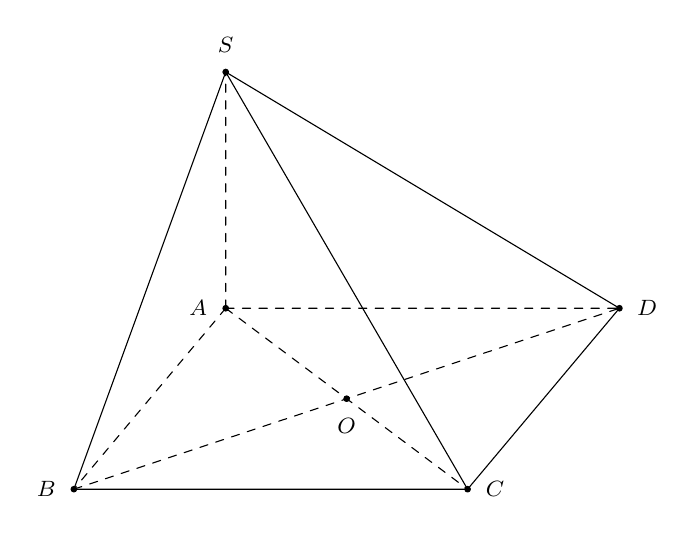
\begin{tikzpicture}[>=stealth,line join=round,line cap=round,font=\footnotesize,scale=1]
      \path (0,0) coordinate (B)
      ++(0:5)  coordinate (C)
      ++(50:3) coordinate (D) 
       ++(180:5) coordinate (A)
      ++(90:3)  coordinate (S);
     \coordinate (O) at (intersection  of A--C and B--D);
      \draw (B)--(C)--(D)--(S)--cycle (S)--(C);
      \draw[dashed] (A)--(B)
      (A)--(S) 
       (A)--(D)
      (B)--(D) 
       (A)--(C);
     \foreach \x/\y in {A/-180,B/-180,C/0,S/90,O/-90,D/0 
      }{\draw[fill=black] (\x) circle (1pt)++(\y:0.35) node{$\x$};} 
    \end{tikzpicture}
  \end{center}
  \begin{itemchoice}
    \itemch {Đúng}. Vì $\heva{
   &BD\perp (SAC)\\ 
    &BD\subset (SBD)}$
   $\Rightarrow (SAC)\perp (SBD)$.\\ 
   \itemch  {Đúng}. Vì $\heva{
   &AC\perp SA\\ 
   &AD\perp  SA\\
   &AC\subset  (SAC), AD\subset(SAD)\\
   & (SAC)\cap (SAD)=SA.}$ \\$ \Rightarrow  ((SAC),(SAD))=(AC,AD)=\widehat{CAD}=45^{\circ}$.
   \itemch {Đúng}. Vì  $\heva{
    &BC\perp (SAB)&\\
   &BC\subset (SBC)}$ 
   $\Rightarrow  (SAB)\perp (SBC)$.
   \itemch {Đúng}.  Vì $\heva{
   &CD\perp  (SAD)\\
   &CD\subset (SCD)}$ 
    $\Rightarrow (SAD)\perp (SCD)$.
  \end{itemchoice}
  }
\end{ex}

% nguồn: Ok_dungsai_lop11_Lan1
\begin{ex}%[1H8H4-3]%[ma:34253059]
 Cho hình chóp $S.ABCD$ có đáy $ABCD$ là hình vuông. Mặt bên $SAB$ là tam giác đều và nằm trong mặt phẳng vuông góc với đáy. Gọi $H$ và $I$ lần lượt là trung điểm của $AB$ và  $BC$. Khi đó
  \choiceTF
  {\True $SH\perp (ABCD)$} 
   {\True $AD\perp (SAB)$}
   {$\left((SAB),(SAD)\right)=60^\circ$}
  {\True  $(SHC)\perp (SDI)$}
  \loigiai{
  \begin{center}
   \begin{tikzpicture}[scale=1,line join=round,font=\footnotesize,line cap=round,thick]
     \coordinate (A) at (0,0); 
     \coordinate  (B) at (-2,-2);
     \coordinate (D)  at (5,0);
     \coordinate (C) at  ($(B)+(D)-(A)$);
      \coordinate (H) at ($(A)!0.5!(B)$);
     \coordinate (S) at  ($(H)+(0,5)$);
     \coordinate (I) at ($(C)!0.5!(B)$); 
     \coordinate  (M) at (intersection of H--C and D--I);
      \draw (S)--(B)
       (S)--(C)
      (B)--(C) 
      (C)--(D) 
       (S)--(D);
      \draw[dashed,thin](H)--(C)
       (A)--(D)
       (S)--(H)
       (I)--(D)
      (S)--(A) 
      (A)--(B); 
     \pic[draw,thin,angle radius=3mm] {right angle  = A--H--S};
     \pic[draw,thin,angle radius=3mm] {right angle = C--H--S}; 
     \pic[draw,thin,angle radius=3mm] {right angle  = D--M--H};
     \foreach \i/\g  in {S/90,A/180,B/-90,C/-90,D/0,H/180,I/-90}{\draw[fill=black](\i) circle (1pt)
       ($(\i)+(\g:3mm)$) node[scale=1]{$\i$};}
    \end{tikzpicture}
  \end{center}
  \begin{itemchoice}
   \itemch{  Đúng.}\\
   Ta có $\heva{&(SAB)\cap (ABCD)=AB\\&(SAB)\perp (ABCD)\\&SH\subset (SAB), SH\perp AB}\Rightarrow  SH \perp (ABCD)$.
   \itemch{ Đúng.}\\ 
   Ta có $\heva{&AD\perp AD\\&AD\perp SH\\&AB,SH\subset  (SAB)}\Rightarrow AD\perp (SAB)$.
    \itemch{ Sai.}\\
   Do $\heva{&AD\perp (SAB)\\&AD\subset (SAD)}\Rightarrow (SAD)\perp  (SAB)$.
   \itemch{ Đúng.}\\ 
   Ta có  $\triangle BCH=\triangle CDI\Rightarrow \widehat{HCB}=\widehat{IDC}$.\\
   Mặt khác $\widehat{IDC}+\widehat{CID}=90^\circ\Rightarrow \widehat{HCB}+\widehat{CID}=90^\circ\Rightarrow HC\perp DI$.\\ 
   Khi đó $\heva{&DI\perp CH\\&DI\perp SH\\&CH,SH\subset (SHC)}\Rightarrow DI\perp (SHC)$, mà  $DI\subset (SDI)$.\\
    Vậy $(SDI)\perp (SHC)$.
  \end{itemchoice}
  }
\end{ex}

% nguồn: Ok_dungsai_lop11_Lan1
\begin{ex}%[1H8V4-3]%[ma:fb497157]
 Cho hình chóp $S.ABCD$ có đáy là hình chữ nhật với $AB=a$, $AD=a\sqrt{3}$. Biết $SA$ vuông góc với mặt phẳng  đáy và $SA=a\sqrt {3}$.
 \choiceTF 
  {\True  $((SAB),(ABCD))=90^{\circ}$}
  {$((SBC),(ABCD))=\widehat{SAB}$} 
   {\True $((SBC),(ABCD))=60^{\circ}$}
   {$((SBD),(ABCD))\approx 69{,}43^{\circ}$}
  \loigiai{
  \begin{center}
   \begin{tikzpicture}[>=stealth,line join=round,line cap=round,font=\footnotesize,scale=1]
      \path (0,0) coordinate (B)
      ++(0:4) coordinate  (C)
      ++(45:2.5) coordinate (D) 
      ++(180:4)  coordinate (A)
      ++(90:3) coordinate  (S);
     \coordinate (K) at ($(B)!0.45!(D)$); 
     \draw (B)--(C)--(D)--(S)--(B)--cycle  (S)--(C);
      \draw[dashed] (A)--(B)
       (A)--(S)
       (A)--(D)
      (B)--(D) 
      (S)--(K) 
      (A)--(K); 
      \foreach \x/\y in {A/-180,B/-180,C/0,S/90,K/0,D/0
      }{\draw[fill=black] (\x) circle (1pt)++(\y:0.35)  node{$\x$};}
      \draw pic[draw,angle radius=2.5mm]{right angle=S--A--D};
     \draw pic[draw,angle  radius=2.5mm]{right angle=B--A--D};
     \draw  pic[draw,angle radius=2.5mm]{right angle=A--K--B};
    \end{tikzpicture}
  \end{center}
  \begin{itemchoice}
   \itemch {Đúng}. Vì  $\heva{
   &SA\perp  (ABCD)\\
   &SA\subset (SAB)}$ 
   $\Rightarrow (SAB)\perp  (ABCD)$.\\
    Hay $((SAB),(ABCD))=90^{\circ}$.
   \itemch {Sai}.  $\heva{
   &BC\perp AB\\ 
   &BC\perp SA(\text{do }SA\perp (ABCD))} 
   \Rightarrow BC\perp (SAB)\Rightarrow BC\perp  SB$.\\
   Khi đó $\heva{ 
   &BC=(SBC)\cap (ABCD)\\ 
   &AB\perp BC,SB\perp  BC\\
    &AB\subset (ABCD),SB\subset (SBC).}$\\
    $\Rightarrow ((SBC),(ABCD))=(SB,AB)=\widehat{SBA}$ (góc $\widehat{SBA}$ nhọn vì $\widehat{SAB}=90^{\circ}$).
   \itemch  {Đúng}. Vì
   tam giác  $SAB$ vuông tại $A$ có $\tan\widehat{SBA}=\dfrac{SA}{AB}=\dfrac{a\sqrt {3}}{a}=\sqrt{3}$.\\ $\Rightarrow\widehat{SBA}=60^{\circ}$.\\
    Vậy $((SBC),(ABCD))=\widehat{SBA}=60^{\circ}$.
    \itemch {Sai}.
   Kẻ đường cao $AK$ của  tam giác $ABD$\\
   Ta có $\heva{ 
   &BD\perp AK\\ 
   &BD\perp  SA}
   \Rightarrow BD\perp (SAK)  \Rightarrow BD\perp SK$.\\
    Khi đó $\heva{
   &(SBD)\cap  (ABCD)=BD\\
    &AK\perp BD,SK\perp BD\\
   &AK\subset  (ABCD),SK\subset (SBD).}$\\
   $\Rightarrow ((SBD),(ABCD))=(SK,AK)=\widehat{SKA}$ (góc $\widehat{SKA}$ nhọn vì  $\widehat{SAK}=90^{\circ}$).\\
   Tam giác $ABD$ vuông tại $A$ có đường cao  $AK$ nên\\
   $\dfrac{1}{AK^2}=\dfrac{1}{AB^2}+\dfrac{1}{AD^2}=\dfrac{1}{a^2}+\dfrac{1}{3a^2}=\dfrac{4}{3a^2}\Rightarrow AK=\dfrac{a\sqrt{3}}{2}$.\\ 
   Tam giác $SAK$ vuông  tại $A$ có $\tan\widehat{SKA}=\dfrac{SA}{AK}=\dfrac{a\sqrt 3}{\dfrac{a\sqrt {3}}{2}}=2\Rightarrow\widehat{SKA}\approx63,43^{\circ}$.\\
   Vậy $((SBD),(ABCD))=\widehat{SKA}\approx63,43^{\circ}$. 
  \end{itemchoice}
  }
\end{ex}

% nguồn: Ok_dungsai_lop11_Lan1
\begin{ex}%[1H8V4-3]%[ma:02f836ab]
 Cho hình  chóp tứ giác đều $S.ABCD$ có cạnh đáy bằng $a$, tâm của đáy là $O$ với $SO=\dfrac{a\sqrt 3}{2}$. Gọi $M$, $N$ lần lượt là trung điểm cạnh $AD$ và $BC$.
 \choiceTF 
  {\True  $(SMN)\perp (ABCD)$}
   {\True $(SAD)\perp (SMN)$}
   {$((SBC),(ABCD))=30^{\circ}$}
   {$((SBC),(SCD))\approx 80{,}52^{\circ}$}
 \loigiai{ 
  \begin{center}
   \begin{tikzpicture}[>=stealth,line join=round,line cap=round,font=\footnotesize,scale=1]
     \path  (0,0) coordinate (D)
      ++(0:5) coordinate (C) 
      ++(50:3) coordinate  (B)
      ++(180:5) coordinate (A) 
       ++(75:4.5) coordinate (S);
     \coordinate (O)  at (intersection of A--C and B--D);
     \coordinate (I) at  ($(S)!0.6!(C)$);
     \coordinate (M)  at ($(A)!0.5!(D)$);
     \coordinate (N) at  ($(B)!0.5!(C)$);
      \draw (D)--(C)--(B)--(S)--cycle (S)--(C)
      (I)--(D) 
      (I)--(B) 
       (S)--(N);
      \draw[dashed] (A)--(B)
      (A)--(S) 
      (A)--(D) 
       (B)--(D)
       (A)--(C)
       (M)--(N)
       (O)--(I)
      (S)--(M) 
       (S)--(O);
     \foreach  \x/\y in {A/45,B/0,C/0,S/90,O/-90,D/-180,M/-45,N/0,I/45
      }{\draw[fill=black] (\x) circle (1pt)++(\y:0.35)  node{$\x$};}
     \draw  pic[draw,angle radius=2.5mm]{right angle=S--O--A};
      \draw pic[draw,angle radius=2.5mm]{right angle=D--I--C};
    \end{tikzpicture}
  \end{center}
  \begin{itemchoice}
   \itemch {Đúng}. Vì $S.ABCD$ là hình chóp tứ giác đều có $O$ là tâm của đáy nên $SO\perp (ABCD)$  Mặt khác $MN$ là đường trung bình của hình vuông $ABCD$ nên $MN$ qua $O$.\\
   Vậy  $SO\subset (SMN)\Rightarrow(SMN)\perp (ABCD)$.
   \itemch  {Đúng}. Vì ta có $\heva{
   &AD\perp MN\\ 
   &AD\perp SO 
   }\Rightarrow AD\perp  (SMN)$.\\
   mà $AD\subset  (SAD)\Rightarrow(SAD)\perp (SMN)$.
   \itemch {Sai}.  Vì ta có $\heva{
    &BC\parallel AD\\
    &AD\perp (SMN)
    }$
   $\Rightarrow BC\perp (SMN)\Rightarrow BC\perp MN$.\\ 
   Khi đó $\heva{ 
   &(SBC)\cap  (ABCD)=BC\\
   &ON\perp  BC,SN\perp BC\\
   &ON\subset  (ABCD),SN\subset (SBC).}
    $\\
    $\Rightarrow((SBC),(ABCD))=(SN,ON)=\widehat{SNO}$\\
   Vì $ON$  là đường trung bình tam giác $ABC$ nên $ON=\dfrac{AB}{2}=\dfrac{a}{2}$.\\
   Tam giác $SON$ vuông tại $O$ có\\ $\tan\widehat{SNO}=\dfrac{SO}{ON}=\dfrac{\dfrac{a\sqrt 3}{2}}{\dfrac{a}{2}}=\sqrt  3\Rightarrow\widehat{SNO}=60^{\circ}$\\
    Vậy $((SBC),(ABCD))=\widehat{SNO}=60^{\circ}$.
   \itemch {Sai}. Vì 
    Kẻ đường cao $DI$ của tam giác $SCD$\\
   Ta có  $\heva{
   &SC\perp  DI\\
   &SC\perp BD(\text{do }BD\perp (SAC))}$ 
    $\Rightarrow SC\perp (IBD)\Rightarrow SC\perp BI$.\\
   Mặt khác $SC=(SBC)\cap  (SCD)$ nên $((SBC),(SCD))=(ID,IB)$\\
    Ta có $\heva{
    &BC\parallel AD\\
   &AD\perp  (SMN)}$
   $\Rightarrow  BC\perp (SMN)\Rightarrow BC\perp MN$.\\
   Khi đó $\heva{ 
   &(SBC)\cap  (ABCD)=BC\\
   &ON\perp  BC,SN\perp BC\\
   &ON\subset (ABCD),SN\subset  (SBC).}$\\
    $\Rightarrow((SBC),(ABCD))=(SN,ON)=\widehat{SNO}$.\\
   Vì $ON$ là đường trung bình tam  giác $ABC$ nên $ON=\dfrac{AB}{2}=\dfrac{a}{2}$.\\
   Tam giác $SON$ vuông tại $O$ có $\tan\widehat{SNO}=\dfrac{SO}{ON}=\dfrac{\dfrac{a\sqrt  3}{2}}{\dfrac{a}{2}}=\sqrt 3 \Rightarrow\widehat{SNO}=60^{\circ}$.\\
    Vậy $((SBC),(ABCD))=\widehat{SNO}=60^{\circ}$.\\
   Kẻ đường cao $DI$ của tam giác  $SCD$.\\
    Ta có $\heva{
   &SC\perp DI\\ 
   &SC\perp BD(\text{do  }BD\perp (SAC))}$
   $\Rightarrow SC\perp (IBD)\Rightarrow SC\perp BI$.\\ 
   Mặt khác $SC=(SBC)\cap  (SCD)$ nên $((SBC),(SCD))=(ID,IB)$.\\
   Ta có $IO\perp BD$ và $O$ là  trung điểm $BD$.\\
   nên $\Delta IBD$  cân tại $I$ và $\widehat{OIB}=\widehat{OID}=\dfrac{1}{2}\widehat{BID}$.\\
   Vì  $ABCD$ là hình vuông cạnh $a$ nên $OC=\dfrac{AC}{2}=\dfrac{a\sqrt 2}{2}=OD$.\\
   Tam giác $SOC$ có đường cao\\ 
    $OI=\dfrac{SO\cdot OC}{\sqrt{S{O^2}+O{C^2}}}=\dfrac{a\sqrt{30}}{10}$\\
   Tam giác $IOD$ vuông tại $O$  có\\
   $\tan\widehat{OID}=\dfrac{OD}{OI}=\dfrac{\dfrac{a\sqrt  2}{2}}{\dfrac{a\sqrt{30}}{10}}=\dfrac{\sqrt{15}}{3}$;\\ $\tan\widehat{BID}=\dfrac{2\tan\widehat{OID}}{1-\tan^2\widehat{OID}}=-\sqrt{15}< 0$ nên $\widehat{BID}$ là góc tù.\\
   Vậy  $((SBC),(SCD))=(ID,IB)=180^{\circ}-\widehat{BID}\approx75,52^{\circ}$.
  \end{itemchoice}
 } 
\end{ex}

% nguồn: Ok_dungsai_lop11_Lan1
\begin{ex}%[1H8K4-3]%[ma:05aef27e]
 Cho tứ diện $S.ABC$ có các tam giác $SAB, SAC$ và $ABC$ vuông cân tại $A$, $SA = a$. Gọi $I$ là trung  điểm của $BC$ và $ \alpha $ là góc giữa hai mặt phẳng $(SBC)$ và $(ABC)$.
  \choiceTF
  {\True  $SA \perp BC$}
   {$AI=a\sqrt{2}$}
  {$AI \perp  (SBC)$}
  {\True $\tan \alpha = \sqrt 2  $}
 \loigiai{ 
  \begin{center}
   \begin{tikzpicture}[scale=1,font=\footnotesize,line join=round,line cap=round,>=stealth]
      \path
      (0,0) coordinate (A) 
      (3,0) coordinate  (C)
       (1,-1) coordinate (B)
      ($(B)!0.5!(C)$) coordinate  (I)
      ($(A)+(0,3)$)  coordinate (S);
     \draw (B)--(S)--(A)--(B)--(C)--(S)--(I); \draw[dashed]  (C)--(A)--(I);
     \foreach \i/\g in {S/90,A/-135,B/-90,C/-20,I/-45}{ 
      \draw[fill=black] (\i) circle (1.2pt)  +(\g:0.25) node{$\i$};}
     \draw pic[draw,angle eccentricity=1.7,angle  radius=0.4cm]{angle=S--I--A};
     \draw pic[draw,angle radius=2mm]{right  angle=A--I--B};
     \draw pic[draw,angle radius=2mm]{right angle=S--I--C}; 
    \end{tikzpicture}
  \end{center}
  \begin{itemchoice}
    \itemch Ta có
   $$\heva{ &SA \perp AB \\& SA \perp AC } \Rightarrow SA \perp (ABC) \Rightarrow SA \perp BC. (1)$$ 
   \itemch Ta có $AB =  AC = SA = a$; $BC = AB \sqrt{2} = a\sqrt{2}$; $AI = \dfrac{BC}{2} = \dfrac{a\sqrt{2}}{2}$.
    \itemch Sai
   \itemch Do tam giác $ABC$ cân tại $A$ nên $AI \perp BC$. $(2)$\\ 
   Từ $(1)$ và $(2)$  suy ra $BC \perp (SAI) \Rightarrow BC \perp SI$.\\
   Ta có $\heva{&(SBC) \cap (ABC) = BC \\& SI \subset (SBC), SI \perp BC \\& AI \subset (ABC), AI \perp BC }\Rightarrow \left[(SBC), (ABC) \right] = (SI, AI) =  \widehat{SIA}$.\\
   $\tan \alpha = \tan \widehat{SIA} = \dfrac{SA}{AI} = a  \cdot \dfrac{2}{a\sqrt{2}} = \sqrt{2}$.
  \end{itemchoice}
  }
\end{ex}


%%%%%%%%%%%%%%%% TRẢ LỜI NGẮN %%%%%%%%%%%%%%%%

% nguồn: Ok_TraLoiNgan_Lop11_Lan1
\begin{ex}%[1H8H4-3]%[ma:b984dc4f]
	Cho hình chóp $S.ABC$ có đáy là tam giác vuông cân tại $B$, $SA\perp (ABC)$, $AB=BC=a$, $SA=a\sqrt{3}$. Tính góc giữa hai  mặt phẳng $(SBC)$ và $(ABC)$ (làm tròn kết quả đến hàng đơn vị của độ).\\
	\shortans{60} 
	 \loigiai{
	\immini{Ta có $\heva{&SA\perp BC\\&AB\perp BC}\Rightarrow BC\perp (SAB)\Rightarrow BC\perp SB$.\\ 
		Mặt  khác $\heva{&(SBC)\cap (ABC)=BC\\&SB\perp BC, SB\subset (SBC)\\&AB\perp BC, AB\subset (ABC)\\&SB\cap AB=B}$\\
		$\Rightarrow  \left((SBC),(ABC)\right)=(SB,AB)=\widehat{SBA}$.\\
		Xét tam giác  $SAB$ vuông tại $A$, có\\ $\tan\widehat{SBA}=\dfrac{SA}{AB}=\sqrt{3}\Rightarrow \widehat{SBA}=60^\circ$.}
		{\begin{tikzpicture}[scale=1,line join=round,font=\footnotesize,line cap=round]
		\coordinate (A) at  (-2,0);
		\coordinate (B) at (1,-2); 
		\coordinate  (C) at (3,0);
		\coordinate (S) at  ($(A)+(0,4)$);
		\draw (S)--(A) 
			 (S)--(B)
			(S)--(C) 
			(B)--(C) 
			 (A)--(B);
		 \draw[dashed,thin](A)--(C);
		\pic[draw,thin,angle radius=3mm] {right angle = S--A--B} pic[draw,thin,angle radius=3mm] {right angle  = S--A--C}pic[draw,thin,angle radius=3mm] {right angle = C--B--A};
		\foreach  \i/\g in {S/90,A/180,B/-90,C/0}{\draw[fill=black](\i) circle (1pt)
			($(\i)+(\g:3mm)$) node[scale=1]{$\i$};} 
	\end{tikzpicture}
		 }
	} 
\end{ex}

% nguồn: Ok_TraLoiNgan_Lop11_Lan1
\begin{ex}%[1H8H4-3]%[ma:18bc7b82]
	Cho hình lập  phương $ABCD.A'B'C'D'$ có $O$, $O'$ lần lượt là tâm của các hình vuông $ABCD$ và $A'B'C'D'$. Góc giữa hai mặt phẳng $(A'BD)$ và $(ABCD)$ bằng bao nhiêu độ? (kết quả làm tròn đến chữ số thập phân thứ nhất).
	 \shortans{54,7}
	 \loigiai{
	 \immini{
		 Ta có $\heva{&BD\perp AO\\&BD\perp AA'}\Rightarrow BD\perp (AA'O)\Rightarrow BD\perp A'O$.\\
		Khi đó $\heva{&A'O\perp BD\\&AO\perp BD\\&(A'BD)\cap (ABCD)=BD}$\\ 
		$\Rightarrow \left((A'BD),(ABCD)\right)=(A'O,AO)=\widehat{A'OA}$.\\ 
		Xét tam  giác $A'AO$ vuông tại $A$, ta có $$\tan\widehat{A'OA}=\dfrac{A'A}{AO}=\dfrac{A'A}{\dfrac{AC}{2}}=\dfrac{A'A}{\dfrac{A'A\sqrt{2}}{2}}=\sqrt{2}.$$
		Do đó $\widehat{A'OA}\approx 54{,}7^\circ$.}{\begin{tikzpicture}[scale=1,line join=round,font=\footnotesize,line cap=round]
		\def\a{3.5} 
		\path (0:0)  coordinate (A)
			 ++(0:\a) coordinate (D)
			++(-130:\a/2) coordinate  (C)
			($(A)+(C)-(D)$) coordinate  (B)
			($(A)+(90:\a)$) coordinate  (A')
			($(B)+(90:\a)$)  coordinate (B')
			($(C)+(90:\a)$) coordinate  (C')
			 ($(D)+(90:\a)$) coordinate (D');
		\path ($(A)!0.5!(C)$) coordinate  (O);
		\path ($(A')!0.5!(C')$)  coordinate (O');
		\draw[dashed] (B)--(A)--(D) 
			(A)--(A') 
			(B)--(A')--(D)--cycle  (C)--(A)--(A')--(O);
		 \draw (A')--(C')
			(B')--(D') 
			(C)--(C') 
			(D)--(D') 
			 (B)--(B')
			(B)--(C)--(D) 
			(A')--(B')--(C')--(D')--cycle; 
		\foreach \x/\g  in {A/180,B/180,C/0,D/0,A'/180,B'/180,C'/0,D'/0,O/-90,O'/90}
		\fill[black] (\x) circle (1pt) 
			($(\g:4mm)+(\x)$) node  {$\x$};
	\end{tikzpicture}
		} 
	} 
\end{ex}

% nguồn: Ok_TraLoiNgan_Lop11_Lan1
\begin{ex}%[1H8H4-3]%[ma:3eda8044]
	Cho lăng trụ đứng tam giác $ABC.A'B'C'$ có đáy $ABC$ là tam giác vuông cân tại $B$. Cho $AB=a$, $AA'=a\sqrt{3}$. Tính số đo góc giữa hai mặt phẳng $(A'BC)$ và $(ABC)$ theo đơn vị độ. 
	\shortans{60} 
	 \loigiai{
	\immini{Vì lăng trụ đã cho là lăng trụ đứng  và tam giác $(ABC)$ vuông ở $B$ nên $BC\perp A'B$.\\
		Từ $(A'BC) \cap (ABC)=BC$, $AB\perp BC$, $A'B \perp BC$ suy ra góc giữa hai  mặt phẳng $(A'BC)$ và $(ABC)$ bằng góc $\widehat{A'BA}=\varphi$.\\
		Ta có  $\tan\varphi=\dfrac{AA'}{AB}=\dfrac{a\sqrt{3}}{a}=\sqrt{3}$.\\
		Vậy  $\varphi=60^\circ$.
		 }{
		\begin{tikzpicture}[scale=1,font=\footnotesize,line join=round,line cap=round,>=stealth]
				 \path (0,0) coordinate (A)
					(3,0)  coordinate (C)
					(2,-1) coordinate (B) 
					(0,3) coordinate  (h);
				\foreach \p in {A,B,C}{\draw  (\p)--(\p)--+(h) coordinate (\p');}
				 \draw (A')--(B')--(C')--cycle (A)--(B)--(C)
					 (A')--(B);
				\draw[dashed] (A)--(C)--(A'); 
				\foreach \p/\g  in {A/180,B/-90,C/0,A'/180,B'/-30,C'/0} \fill[black] (\p) circle (1pt)+(\g:0.3) node{$\p$};
				\foreach \x/\y/\z in {A/B/C,A'/A/B,A'/A/C}\draw pic[draw,angle  radius=0.2cm]{right angle=\x--\y--\z};
			\end{tikzpicture}
		} 
	} 
\end{ex}

% nguồn: Ok_TraLoiNgan_Lop11_Lan1
\begin{ex}%[1H8H4-3]%[ma:6d05a9e6]
	Cho hình chóp $S.ABCD$ có $ABCD$ là hình thang vuông tại $A$, $AB=BC=a$, $AD=2a$ và hai mặt bên $(SAB)$, $(SAD)$ cùng vuông góc  với mặt đáy và $SA=a\sqrt{2}$.
	Tính tang của  góc $\varphi$ giữa $(SBC)$ và $(ABCD)$ (làm tròn kết quả đến chữ số thập phân thứ hai).
	\shortans{1,41} 
	\loigiai{ 
	 \immini{
		Ta có $$\heva{&BC\perp AB\\&BC\perp SA}\Rightarrow BC\perp (SAB)\Rightarrow  BC\perp SB.$$
		Khi đó $\heva{&BC=(SBC)\cap (ABCD)\\&SB\perp  BC, SB\subset (SBC)\\&AB\perp BC, AB\subset (ABCD)}$\\
		$\Rightarrow \left((SBC),(ABCD)  \right)=(SB,AB)=\widehat{SBA}$.\\
		Trong tam giác vuông $SBA$, ta có $$\tan\widehat{SBA}=\dfrac{SA}{AB}=\dfrac{a\sqrt{2}}{a}=\sqrt{2}\approx1{,}41.$$}{\begin{tikzpicture}[scale=0.8,line join=round,font=\footnotesize,line cap=round]
		\coordinate (A)  at (0,0);
		\coordinate (B) at  (-2,-2);
		\coordinate  (D) at (6,0);
		\coordinate  (C) at (2,-2);
		\coordinate (S) at  ($(A)+(0,4)$);
		\draw  (S)--(B)
			(S)--(C) 
			(S)--(D) 
			 (B)--(C)--(D);
		\draw[dashed,thin](S)--(A) 
			 (A)--(B)
			(A)--(D); 
		 \pic[draw,thin,angle radius=3mm] {right angle = S--A--D} pic[draw,thin,angle radius=3mm] {right angle = S--A--B}pic[draw,thin,angle radius=3mm] {right angle = B--A--D}pic[draw,thin,angle radius=3mm] {right angle = C--B--A};
		\foreach \i/\g in {S/90,A/-90,B/-90,C/-90,D/0}{\draw[fill=black](\i)  circle (1pt)
			 ($(\i)+(\g:3mm)$) node[scale=1]{$\i$};}
	\end{tikzpicture}
		 }
	} 
\end{ex}

% nguồn: Ok_TraLoiNgan_Lop11_Lan1
\begin{ex}%[1H8H4-3]%[ma:884a421a]
	Cho hình chóp tứ giác đều $S.ABCD$  có cạnh đáy bằng đáy $2a$, đường cao bằng $a\sqrt{2}$. Tính $\tan\varphi$ của góc giữa mặt phẳng $(SCD)$ và $(ABCD)$ (kết quả làm tròn đến số thập phân thứ hai).
	 \shortans{1,41}
	\loigiai{ 
	\immini{ 
		Gọi $O=AC\cap BD$ và $M$ là  trung điểm $CD$.\\
		Ta  có $\heva{&(SCD)\cap (ABCD)=CD\\&OM\perp CD\\&SM\perp CD}$\\
		$\Rightarrow \varphi=(OM,SM)=\widehat{SMO}$.\\ 
		Trong tam giác vuông $SMO$, ta có $$\tan\widehat{SMO}=\dfrac{SO}{OM}=\dfrac{a\sqrt{2}}{a}=\sqrt{2}\Rightarrow \tan\varphi=\sqrt{2}\approx 1{,}41.$$}{\begin{tikzpicture}[scale=0.8,line join=round,font=\footnotesize,line cap=round]
		\coordinate  (A) at (0,0);
		\coordinate (B) at  (-2,-2);
		 \coordinate (D) at (5,0);
		\coordinate (C) at  ($(B)+(D)-(A)$);
		\coordinate  (O) at ($(A)!0.5!(C)$);
		\coordinate (S) at  ($(O)+(0,5)$);
		\coordinate  (M) at ($(C)!0.5!(D)$);
		 \draw (S)--(B)
			 (S)--(C)
			 (B)--(C)
			 (C)--(D)
			 (S)--(D)
			 (S)--(M);
		\draw[dashed,thin](A)--(C) 
			(A)--(D) 
			 (S)--(O)
			(B)--(D) 
			 (S)--(A)
			(A)--(B) 
			(O)--(M); 
		 \pic[draw,thin,angle radius=2mm] {right angle = S--O--D} pic[draw,thin,angle radius=2mm] {right angle = S--O--A};
		\foreach \i/\g in  {S/90,A/180,B/-90,C/-90,D/0,O/-90,M/0}{\draw[fill=black](\i) circle (1pt)
			 ($(\i)+(\g:3mm)$) node[scale=1]{$\i$};}
	\end{tikzpicture}
		} 
	} 
\end{ex}

% nguồn: Ok_TraLoiNgan_Lop11_Lan1
\begin{ex}%[1H8H4-3]%[ma:a8051794]
	Cho hình chóp $S.ABC$ có $SA\perp (ABC),SA=1$ và đáy $ABC$ là tam giác đều với độ dài cạnh bằng $2$. Tính góc giữa mặt phẳng $(SBC)$  và mặt phẳng $(ABC)$.
	 \shortans{30}
	\loigiai{ 
	\immini{ 
		Gọi  $I$ là trung điểm của $BC$ . Khi đó, ta có\\
		 $\heva{
		&BC\perp  SA\\
		&BC\perp AI}\Rightarrow BC\perp (SIA)\Rightarrow BC\perp  SI$.\\
		 Ta có
		$\heva{ 
		&(SBC)\cap (ABC)=BC\\ 
		 &SI\perp BC\\
		 &AI\perp BC\\
		&SI\subset (SBC)\\ 
		&AI\subset (ABC)}$\\ 
		 $\Rightarrow ((SBC),(ABC))=(SI,AI)=\widehat{SIA}$.\\
		Nên $\tan\widehat{SIA}=\dfrac{SA}{IA}=\dfrac{1}{\sqrt  3}$.\\
		Suy ra $\widehat{SIA}=30^{\circ}$  nên $\widehat{((SBC),(ABC))}=30^{\circ}$.}
		{	\begin{tikzpicture}[>=stealth,line join=round,line cap=round,font=\footnotesize,scale=1]
		\path (0,0) coordinate (A) 
			++(-55:2.5) coordinate (B) 
			++(30:4) coordinate (C) 
			++(145:5.7)  coordinate (S);
		\coordinate (I) at ($(B)!0.5!(C)$); 
		\draw  (A)--(B)--(C)--(S)--cycle (S)--(I)
			 (S)--(B);
		\draw[dashed]  (A)--(C)
			(A)--(I); 
		\foreach  \x/\y in {A/-180,B/-90,C/40,S/90,I/-45
			}{\draw[fill=black] (\x) circle  (1pt)++(\y:0.35) node{$\x$};}
		 \draw pic[draw,angle radius=2.5mm]{right angle=B--A--S};
		\draw pic[draw,angle radius=2.5mm]{right  angle=C--A--S};
	\end{tikzpicture}
	}} 
\end{ex}

% nguồn: Ok_TraLoiNgan_Lop11_Lan1
\begin{ex}%[1H8H4-3]%[ma:26ef40ec]
	Cho hình chóp $S.ABCD$ có đáy $ABCD$ là hình vuông và $SA$ vuông góc với mặt phẳng $(ABCD)$. Góc giữa hai mặt phẳng $(SCD)$ và $(ABCD)$ là $\widehat{mnq}$, (theo bảng $24$ chữ cái tiếng anh) gọi $m$ là thứ tự của chữ cái $x$, $n$ là thứ tự của chữ cái $y$, $q$ là thứ tự của chữ  cái $z$. Hãy tính tống $m+n+q$.
	\shortans{24} 
	 \loigiai{
	 \immini{
		$(SCD)\cap (ABCD)=CD$.\\ 
		Ta có $\heva{ 
		&{CD\perp AD}\\ 
		 &{CD\perp SA}}
		 \Rightarrow CD\perp SD$.\\
		nên góc giữa hai mặt  phẳng $(SCD)$ và $(ABCD)$ là góc giữa $AD$ và $SD$ là góc $\widehat{SDA}$.\\
		Theo  bảng chữ cái $m=19$, $n=4$, $q=1$.\\
		Vậy $m+n+q=24$.} 
		{	\begin{tikzpicture}[>=stealth,line join=round,line cap=round,font=\footnotesize,scale=0.9]
		\path (0,0)  coordinate (B)
			++(0:5) coordinate  (C)
			++(50:2.5) coordinate (D) 
			++(180:5)  coordinate (A)
			++(90:3.5) coordinate  (S);
		\draw  (B)--(C)--(D)--(S)--cycle (S)--(C);
		\draw[dashed]  (A)--(B)
			 (A)--(S)
			(A)--(D); 
		\foreach \x/\y in {A/-180,B/-180,C/0,S/90,D/0 
			}{\draw[fill=black] (\x) circle  (1pt)++(\y:0.35) node{$\x$};}
		\draw pic[draw,angle radius=2.5mm]{right  angle=S--A--B};
	\end{tikzpicture}
	}} 
\end{ex}

% nguồn: Ok_TraLoiNgan_Lop11_Lan1
\begin{ex}%[1H8V4-3]%[ma:70ff415e]
	Cho hình chóp đều $S.ABCD$ có độ dài cạnh đáy bằng $a$, $SA=\dfrac{a\sqrt{3}}{2}$. Góc giữa mặt bên  và mặt đáy bằng bao nhiêu độ?
	 \shortans{45}
	\loigiai{ 
	\immini{Gọi $O$ là tâm hình vuông $ABCD$,  ta có $SO\perp (ABCD)$. Gọi $M$ là trung điểm $AB$, khi đó $AB\perp (SOM)$. Do đó, góc giữa mặt bên $(SAB)$ và mặt đáy $(ABCD)$ là góc $\widehat{SMO}$.\\
		 Ta có
		\begin{align*}
			 SO=&\sqrt{SA^2-AO^2}\\
			 =&\sqrt{\left(\dfrac{a\sqrt{3}}{2}\right)^2-\left(\dfrac{a\sqrt{2}}{2}\right)^2}=\dfrac{a}{2};\\
			 MO=&\dfrac{AD}{2}=\dfrac{a}{2}.
		\end{align*}
		 Vậy $\tan\widehat{SMO}=\dfrac{SO}{MO}=\dfrac{a}{2}:\dfrac{a}{2}=1\Rightarrow\widehat{SMO}=45^\circ$.
		}{ 
		\begin{tikzpicture}[line cap=round,line join=round,>=stealth,scale=.8]
				 \path
					(0,0) coordinate (A) 
					 ($(A)+(-2,-1)$) coordinate (B)
					 ($(A)+(4,0)$) coordinate (D)
					($(B)+(D)-(A)$)  coordinate (C)
					($(A)!1/2!(C)$) coordinate  (O)
					($(O)+(0,4)$) coordinate (S) 
					($(A)!1/2!(B)$) coordinate (M); 
				 \draw[dashed](S)--(A)--(B)
					(A)--(D) 
					 (S)--(M)--(O)--cycle;
				\draw  (S)--(B)--(C)--(D)--cycle (S)--(C);
				\foreach  \p/\n in {S/above,A/left,B/below,C/below,D/right,M/below,O/below}
				\fill (\p)  circle (1pt) node[\n]{$\p$};
			\end{tikzpicture}
		} 
	} 
\end{ex}

% nguồn: Ok_TraLoiNgan_Lop11_Lan1
\begin{ex}%[1H8V4-3]%[ma:8c727588]
	Cho hình chóp $S.ABC$ có đáy $ABC$  là tam giác vuông tại $B$. Cạnh bên $SA$ vuông góc với mặt phẳng đáy. Góc giữa mặt phẳng $(SBC)$ và mặt phẳng $(ABC)$ là $\widehat{xyz}$, (theo bảng $24$ chữ cái tiếng anh) gọi $a$ là thứ tự của chữ cái $x$, $b$ là thứ tự của chữ cái $y$, $c$ là thứ tự của chữ cái $z$. Hãy tính tống $a+b+c$.
	 \shortans{22}
	\loigiai{ 
	\immini{ 
		Do $AB$ là hình chiếu của $SB$ trên $(ABC)$ mà $AB\perp BC\Rightarrow SB\perp BC$ (định lí 3 đường vuông góc).\\ 
		Ta có $\heva{ 
		&(SBC)\cap (ABC)=BC\\ 
		&SB\subset (SBC);SB\perp BC\\ 
		&AB\subset (ABC);AB\perp BC.}$\\ 
		Góc  giữa mặt phẳng $(SBC)$ và mặt phẳng $(ABC)$ là $(SB,AB)=\widehat{SBA}$.\\
		 Theo bảng chữ cái $a=19$, $b=2$, $c=1$.\\
		Vậy  $a+b+c=22$.}
		{	\begin{tikzpicture}[>=stealth,line join=round,line cap=round,font=\footnotesize,scale=1]
		 \path (0,0) coordinate (A)
			++(-45:2.5) coordinate (B) 
			++(30:3) coordinate  (C)
			++(140:5.8) coordinate (S); 
		 \draw (A)--(B)--(C)--(S)--cycle (S)--(B);
		\draw[dashed] (A)--(C); 
		 \foreach \x/\y in {A/-180,B/-90,C/40,S/90
			}{\draw[fill=black] (\x) circle  (1pt)++(\y:0.35) node{$\x$};}
		\draw pic[draw,angle radius=2.5mm]{right  angle=B--A--S};
		 \draw pic[draw,angle radius=2.5mm]{right angle=C--A--S};
		\draw pic[draw,angle radius=2.5mm]{right  angle=A--B--C};
	\end{tikzpicture}
		 }
	 }
\end{ex}

% nguồn: Ok_TraLoiNgan_Lop11_Lan1
\begin{ex}%[1H8V4-3]%[ma:2c941fce]
	Cho hình chóp $S.ABCD$ có đáy $ABCD$ là hình chữ nhật $AB=a$, $AD=a\sqrt{3}$. Cạnh bên $SA$ vuông góc với đáy và $SA=a$. Gọi $\alpha=((SCD),(ABCD))$ và  $\beta = ((SBC),(SAD))$. Khi đó $\alpha + \beta$ bằng.
	\shortans{75} 
	\loigiai{ 
		\begin{center}
			\begin{tikzpicture}[>=stealth,line join=round,line cap=round,font=\footnotesize,scale=1]
					\path (0,0) coordinate  (B)
						++(0:5) coordinate (C) 
						++(50:3)  coordinate (D)
						++(180:5) coordinate (A) 
						++(90:3)  coordinate (S)
						++(0:4)  coordinate (M)
						++(0:-5)  coordinate (N);
					\coordinate (x)  at (5.5,5.3);
					\draw (B)--(C)--(D)--(S)--cycle (S)--(C) 
						(N)--(M); 
					\draw[dashed]  (A)--(B)
						(A)--(S) 
						 (A)--(D);
					\foreach \x/\y in {A/-180,B/-180,C/0,S/90,D/0 
						}{\draw[fill=black]  (\x) circle (1pt)++(\y:0.35) node{$\x$};}
					\draw pic[draw,angle radius=2.5mm]{right  angle=S--A--B};
					\path (x)  node [above]{$x$};
				\end{tikzpicture}
		\end{center}
		$\heva{ 
		&CD\perp  AD\\
		&CD\perp SA (\text{do  }SA\perp (ABCD))}$
		 $\Rightarrow CD\perp (SAD)\Rightarrow CD\perp SD$.\\
		 $\heva{
		&(SCD)\cap (ABCD)=CD\\ 
		&AD\perp CD, \, SD\perp  CD\\
		&AD\subset (ABCD),SD\subset (SCD).}$ 
		$\Rightarrow ((SCD),(ABCD))=(SD,AD)=\widehat{SDA}$.\\ 
		Tam giác  $SAD$ vuông tại $A$ có\\
		$\tan\widehat{SDA}=\dfrac{SA}{AD}=\dfrac{a}{a\sqrt  {3}}=\dfrac{\sqrt {3}}{3}\Rightarrow\widehat{SDA}=30^{\circ}$.\\
		Vậy  $((SCD),(ABCD))=\widehat{SDA}=30^{\circ}$ .\\
		Ta có $\heva{ 
		&S\in (SAD)\cap (SBC)\\ 
		&AD\parallel BC\\ 
		&AD\subset (SAD),BC\subset  (SBC)}$
		$\Rightarrow  (SAD)\cap (SBC)=S_x\parallel AD\parallel BC$.\\
		Ta có $\heva{ 
		&SA\perp  AD\\
		&Sx\parallel AD}\Rightarrow SA\perp  S_x$. \\
		Lại  có $\heva{
		&S_x\perp  SA\\
		&S_x\perp AB (\text{do  }S_x\parallel AD,AD\perp AB)}$
		$\Rightarrow  S_x\perp (SAB)\Rightarrow S_x\perp SB$.\\
		Khi  đó $\heva{
		 &(SBC)\cap (SAD)=S_x\\
		&SB\perp S_x,SA\perp  S_x\\
		&SB\subset  (SBC),SA\subset (SAD)}$
		$\Rightarrow ((SBC),(SAD))=(SB,SA)=\widehat{ASB}$.\\ 
		Tam giác $SAB$ vuông cân tại $A$ nên  $\widehat{ASB}=45^{\circ}$.\\
		Vậy  $((SBC),(SAD))=\widehat{ASB}=45^{\circ}$.
	 }
\end{ex}

% nguồn: Ok_TraLoiNgan_Lop11_Lan1
\begin{ex}%[1H8V4-3]%[ma:2547ce37]
	 Cho hình lập phương $ABCD.A'B'C'D'$. Tính góc giữa hai mặt phẳng $(AB'C')$ và $(AC'D')$.
	\shortans{60} 
	 \loigiai{
		\begin{center}
			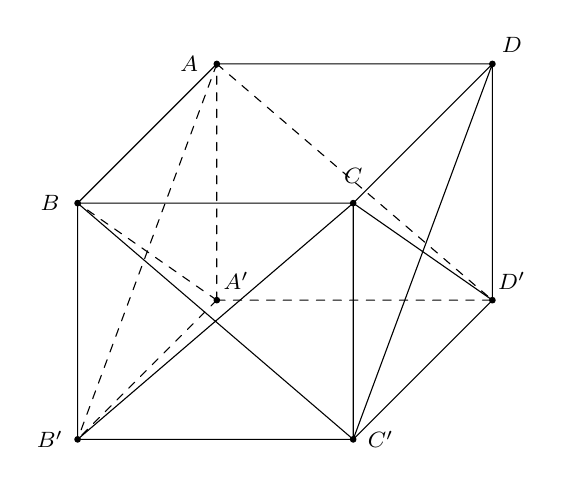
\begin{tikzpicture}[>=stealth,line join=round,line cap=round,font=\footnotesize,scale=1]
					\path (0,0) coordinate  (B')
						++(0:3.5) coordinate (C') 
						++(45:2.5)  coordinate (D')
						 ++(180:3.5) coordinate (A')
						++(90:3) coordinate (A) 
						++(0:3.5) coordinate (D) 
						 ++(-135:2.5) coordinate (C)
						++(-180:3.5) coordinate  (B);
					\coordinate (I) at  (intersection of A--B' and B--A');
					 \coordinate (K) at (intersection of C--D' and D--C');
					\coordinate (L) at (intersection of B--C' and  C--B');
					 \draw (B)--(C)--(D)--(A)--(B)
						(B)--(B')--(C')--(D')--(D) 
						 (C')--(C)
						 (B)--(B')
						(C)--(D') 
						(D)--(C') 
						 (B)--(C')
						(C)--(B'); 
					\draw[dashed] (A')--(A) 
						(A')--(B') 
						(A')--(B') 
						(A')--(B) 
						 (A)--(D')
						(A')--(D') 
						 (A)--(B')
						(A)--(B'); 
					\foreach  \x/\y in {A/-180,B/-180,C/90,D/45,{A'}/45,{D'}/45,{C'}/0,{B'}/-180
						}{\draw[fill=black] (\x) circle (1pt)++(\y:0.35)  node{$\x$};}
				\end{tikzpicture}
		\end{center}
		Vì $ABCD\cdot A'B'C'D'$ là  hình lập phương nên $BC\perp(ABB'A')\Rightarrow BC\perp AB'$. \qquad(1)\\
		Mặt khác $A'B\perp AB'$ (hai đường chéo trong  hình vuông). \qquad(2)\\
		Từ $(1)$ và $(2)$ suy ra $AB'\perp(BCD'A')$.\\ 
		Mà $A{B'}\subset(ADC'B')$ nên $(ADC'B')\perp(BCD'A')$.\\ 
		Nhận  xét $(AB'C')\equiv(ADC'B'),(AC'D')\equiv(ABC'D')$.\\
		Ta  có $\heva{
		&CD'\bot C'D\\ 
		&CD'\perp AD \,  (\text{do }AD\perp(CDD'C'))}
		 \Rightarrow CD'\perp(ADC'B')$ \qquad(3)\\
		Tương tự  $\heva{
		 &B'C\perp BC'\\
		 &B'C\perp AB(\text{do }AB\perp(BCC'B'))}
		\Rightarrow B'C\perp(ABC'D')$. \qquad(4)\\ 
		Từ $(3)$  và $(4)$ suy ra $((AB'C'),(AC'D'))=(CD',CB')$.\\
		Giả sử cạnh hình lập phương bằng  $a$.\\
		 Ta có $CB'=CD'=B'D'=a\sqrt{2}$ (đường chéo trong hình vuông).\\
		Suy ra  tam giác $CB'D'$ đều.\\
		Do vậy  $((AB'C'),(AC'D'))=(C{D'},C{B'})=\widehat{B'CD'}=60^{\circ}$.
	 }
\end{ex}

% nguồn: Ok_TraLoiNgan_Lop11_Lan1
\begin{ex}%[1H8V4-3]%[ma:cf09e366]
	Cho hình lăng  trụ tam giác đều $ABC.A'B'C'$ có cạnh đáy bằng $a$ và cạnh bên bằng $\dfrac{3a}{2}$. Tính góc giữa hai mặt phẳng $(A'B'C)$ và $(ABC)$?
	 \shortans{60}
	 \loigiai{
	\immini{ 
		Ta  có $(ABC)\cap\left(A'BC\right)=BC$.\\
		Gọi trung điểm của  cạnh $BC$ là $M$.\\
		Tam giác $ABC$ dều nên ta có $AM\perp BC$.  \qquad(1)\\
		$ABC.A'B'C'$ là lăng trụ đều nên $AA'\perp (ABC)\Rightarrow AA'\perp BC$. \qquad(2)\\ 
		Từ $(1)$ và $(2)$ ta suy ra $BC\perp(AA'M)\Rightarrow  BC\bot A'M$.\\
		Suy ra góc $\varphi$  giữa hai mặt phẳng $\left(A'BC\right)$ và $(ABC)$ là góc giữa hai đường thẳng $AM$ và $A'M$.\\
		Vì tam giác $A'AM$ vuông  tại $A$ nên suy ra $\varphi=\widehat{A'MA}$.\\
		Ta có $\tan\varphi=\dfrac{A{A'}}{AM}=\dfrac{\dfrac{3a}{2}}{\dfrac{a\sqrt 3}{2}}=\sqrt  3 $. Suy ra $\varphi=60^{\circ}$.}
		{	\begin{tikzpicture}[>=stealth,line join=round,line cap=round,font=\footnotesize,scale=1]
		 \path (0,0) coordinate (A)
			++(-40:3.5) coordinate (B) 
			 ++(50:2.5) coordinate (C)
			++(90:4) coordinate  (C')
			++(-180:4.15) coordinate  (A')
			++(-40:3.5) coordinate (B'); 
		\coordinate (M) at ($(B)!0.5!(C)$); 
		 \draw (A)--(B)--(C)--(C')--(A')--cycle (A')--(B')
			 (C')--(B')
			(B)--(B'); 
		 \draw[dashed] (A)--(C)
			 (A)--(M)
			 (A')--(M);
		 \foreach \x/\y in {A/-180,B/-90,C/0,{C'}/45,{A'}/-180,{B'}/-135,M/-30
			}{\draw[fill=black]  (\x) circle (1pt)++(\y:0.35) node{$\x$};}
		\draw pic[draw,angle radius=2.5mm]{right angle={A'}--A--M}; 
		\draw pic[draw,angle  radius=2.5mm]{right angle=A--M--B};
	\end{tikzpicture}
		 }
	 }
\end{ex}


%%%%%%%%%%%%%%%% TỰ LUẬN %%%%%%%%%%%%%%%%

% nguồn: Ok_TuanLuan_Toan11_Lan1
\begin{bt}%[1H8H4-3]%[ma:884c090e]
	Cho hình chóp $S.ABCD$ có $SA \perp (ABCD)$, đáy là hình chữ nhật $ABCD$ với $AB  = a$, $AD = a\sqrt{3}$, $SA = 3a$.
	\begin{enumerate}
		\item  Chứng minh tam giác $SBC$ vuông tại $B$.
		\item Gọi $H$ là  hình chiếu vuông góc của $A$ lên cạnh $BD$. Chứng minh $(SAH) \perp (SBD)$.
		\item Tính góc giữa mặt phẳng $(SBD)$ và mặt phẳng  $(SAB)$.
	\end{enumerate}
	\loigiai{ 
		\begin{center}
			\begin{tikzpicture}[>=stealth,line join=round,line cap=round,font=\footnotesize,scale=1]
					\path 
						(-1.5,-2) coordinate (B) 
						(0,0)  coordinate (A)
						(3.5,-2)  coordinate (C)
						($(A)-(B)+(C)$) coordinate (D) 
						(0,3) coordinate (S) 
						($(B)!0.4!(D)$)  coordinate (H)
						($(S)!0.6!(H)$) coordinate  (K);
					\draw (S)--(B)--(C)--(D)--(S)--(C); 
					\draw[dashed]  (S)--(A)--(C)
						(B)--(A)--(D)--(B) 
						 (S)--(H)--(A)--(K)--(D);
					\foreach \d/\g in {A/180,B/-135,D/0,C/-45,S/90,H/-90,K/40} \fill (\d) node[shift={(\g:0.3)}]{$\d$} circle  (1pt);
					\pic[draw,angle radius=2mm,angle eccentricity=1.5] {right angle = S--A--D}; 
					\pic[draw,angle radius=2mm,angle  eccentricity=1.5] {right angle = A--H--B};
					\pic[draw,angle radius=2mm,angle eccentricity=1.5] {right angle = A--K--S}; 
					\pic[draw,angle radius=3mm,angle eccentricity=1.5] {right angle =  A--B--C};
				\end{tikzpicture}
		\end{center}
		`\begin{enumerate}
		\item Ta có $\heva{&BC \perp SA \,\, (SA \perp (ABCD))\\&BC  \perp AB \textrm{ ($ABCD$ là hình chữ nhật)}} \Rightarrow BC \perp (SAB)$.\\
		Mà $SB  \subset (SAB) \Rightarrow BC \perp SB$ hay $\triangle SBC$ vuông tại $B$.
		\item Vì $H$ là hình chiếu vuông góc của  $A$ lên cạnh $BD$ nên $AH \perp BD$.\\
		Ta có $\heva{&BD \perp AH \textrm{ (cmt)}\\&BD \perp  SA \,\, (SA \perp (ABCD))} \Rightarrow BD \perp (SAH)$.\\
		Mà $BD  \subset (SBD)$ nên $(SAH) \perp (SBD)$.
		\item Ta có $\heva{&BC \perp (SAB) \textrm{ (cmt)}\\&BC \parallel AD \textrm{  ($ABCD$ là hình chữ nhật)}} \Rightarrow AD \perp (SAB)$. $\hfill (1)$\\
		Trong  $(SAH)$, kẻ $AK \perp SH$.\\
		Ta có $\heva{&AK \perp SH \textrm{ (cmt)}\\&AK \perp BD \,\,(BD \perp (SAH), AK \subset (SAH))} \Rightarrow AK \perp (SBD)$.  $\hfill (2)$\\
		Từ $(1)$ và $(2)$, suy ra $\left((SBD),(SAB)\right) = \left(AK, AD\right) =  \widehat{KAD}$.\\
		Xét $\triangle ABD$ vuông tại  $A$, có đường cao $AH$, ta có
		$$ \dfrac{1}{AH^2} = \dfrac{1}{AB^2} +  \dfrac{1}{AD^2} \Rightarrow AH^2 = \dfrac{AB^2\cdot AD^2}{AB^2 + AD^2} = \dfrac{a^2\cdot (a\sqrt{3})^2}{a^2 + (a\sqrt{3})^2} = \dfrac{3a^2}{4}. $$
		Suy ra $AH = \dfrac{a\sqrt{3}}{2}$.\\ 
		Ta có $SA \perp (ABCD)$, $AH \subset (ABCD) \Rightarrow SA \perp AH$  nên $\triangle SAH$ vuông tại $A$.\\
		Xét $\triangle  SAH$ vuông tại $A$, có đường cao $AK$, ta có
		$$ \dfrac{1}{AK^2} = \dfrac{1}{AH^2} + \dfrac{1}{SA^2} \Rightarrow AK^2 =  \dfrac{AH^2\cdot SA^2}{AH^2 + SA^2} = \dfrac{\left(\dfrac{a\sqrt{3}}{2}\right)^2\cdot (3a)^2}{\left(\dfrac{a\sqrt{3}}{2}\right)^2 + (3a)^2} = \dfrac{9a^2}{13}. $$
		Suy  ra $AK = \dfrac{3a\sqrt{13}}{13}$.\\
		Vì $AK \perp (SBD)$, $KD \subset (SBD)$ nên  $AK \perp KD$ do đó $\triangle AKD$ vuông tại $K$.\\
		Xét $\triangle  AKD$ vuông tại $K$, ta có\\
		$\cos\widehat{KAD} =  \dfrac{AK}{AD} = \dfrac{\dfrac{3a\sqrt{13}}{13}}{a\sqrt{3}} = \dfrac{\sqrt{39}}{13}$\\
		$\Rightarrow \widehat{KAD} \approx 61^\circ$.\\ 
		Vậy $\left((SBD),(SAB)\right) =  \left(AK, AD\right) = \widehat{KAD} \approx 61^\circ$.
	\end{enumerate}
} 
\end{bt}

% nguồn: Ok_TuanLuan_Toan11_Lan2
\begin{ex}%[1H8H4-3]%[ma:f15396b3]
	Cho hình chóp $S.ABCD$ có $SA \perp (ABCD)$, đáy là hình chữ nhật $ABCD$ với $AB = a$, $AD  = a\sqrt{3}$, $SA = 3a$.
	\begin{enumerate}
		\item Chứng minh tam giác $SBC$ vuông tại  $B$.
		\item Gọi $H$ là hình chiếu vuông góc của $A$ lên cạnh $BD$.  Chứng minh $(SAH) \perp (SBD)$.
		\item Tính góc giữa mặt phẳng $(SBD)$ và mặt  phẳng $(SAB)$.
	\end{enumerate}
	\loigiai{ 
		\begin{center}
			\begin{tikzpicture}[>=stealth,line join=round,line cap=round,font=\footnotesize,scale=1]
					\path 
						 (-1.5,-2) coordinate (B)
						(0,0) coordinate (A) 
						(3.5,-2) coordinate  (C)
						($(A)-(B)+(C)$) coordinate  (D)
						 (0,3) coordinate (S)
						 ($(B)!0.4!(D)$) coordinate (H)
						($(S)!0.6!(H)$)  coordinate (K);
					\draw  (S)--(B)--(C)--(D)--(S)--(C);
					\draw[dashed] (S)--(A)--(C) 
						(B)--(A)--(D)--(B) 
						(S)--(H)--(A)--(K)--(D); 
					\foreach  \d/\g in {A/180,B/-135,D/0,C/-45,S/90,H/-90,K/40} \fill (\d) node[shift={(\g:0.3)}]{$\d$} circle (1pt);
					\pic[draw,angle radius=2mm,angle eccentricity=1.5] {right angle =  S--A--D};
					\pic[draw,angle radius=2mm,angle eccentricity=1.5] {right angle =  A--H--B};
					\pic[draw,angle radius=2mm,angle  eccentricity=1.5] {right angle = A--K--S};
					\pic[draw,angle radius=3mm,angle eccentricity=1.5]  {right angle = A--B--C};
				\end{tikzpicture}
		\end{center}
		`\begin{enumerate}
		\item Ta có $\heva{&BC \perp SA \,\, (SA \perp (ABCD))\\&BC \perp AB \textrm{  ($ABCD$ là hình chữ nhật)}} \Rightarrow BC \perp (SAB)$.\\
		 Mà $SB \subset (SAB) \Rightarrow BC \perp SB$ hay $\triangle SBC$ vuông tại $B$.
		\item Vì $H$ là hình chiếu vuông góc của $A$  lên cạnh $BD$ nên $AH \perp BD$.\\
		Ta có $\heva{&BD \perp AH \textrm{ (cmt)}\\&BD \perp SA \,\, (SA \perp (ABCD))} \Rightarrow  BD \perp (SAH)$.\\
		Mà $BD \subset (SBD)$ nên $(SAH) \perp  (SBD)$.
		\item Ta có $\heva{&BC \perp (SAB) \textrm{ (cmt)}\\&BC \parallel AD \textrm{  ($ABCD$ là hình chữ nhật)}} \Rightarrow AD \perp (SAB)$. $\hfill (1)$\\
		Trong $(SAH)$, kẻ $AK \perp  SH$.\\
		Ta có $\heva{&AK \perp SH \textrm{ (cmt)}\\&AK \perp BD \,\,(BD \perp (SAH),  AK \subset (SAH))} \Rightarrow AK \perp (SBD)$. $\hfill (2)$\\
		Từ $(1)$ và $(2)$, suy ra $\left((SBD),(SAB)\right)  = \left(AK, AD\right) = \widehat{KAD}$.\\
		Xét $\triangle ABD$ vuông tại $A$, có  đường cao $AH$, ta có
		$$ \dfrac{1}{AH^2} = \dfrac{1}{AB^2} + \dfrac{1}{AD^2} \Rightarrow AH^2 = \dfrac{AB^2\cdot AD^2}{AB^2 + AD^2} = \dfrac{a^2\cdot (a\sqrt{3})^2}{a^2 + (a\sqrt{3})^2} =  \dfrac{3a^2}{4}. $$
		Suy ra $AH = \dfrac{a\sqrt{3}}{2}$.\\ 
		Ta có $SA \perp (ABCD)$, $AH \subset (ABCD) \Rightarrow SA  \perp AH$ nên $\triangle SAH$ vuông tại $A$.\\
		Xét $\triangle SAH$  vuông tại $A$, có đường cao $AK$, ta có
		$$ \dfrac{1}{AK^2} = \dfrac{1}{AH^2} + \dfrac{1}{SA^2} \Rightarrow AK^2 = \dfrac{AH^2\cdot SA^2}{AH^2 + SA^2}  = \dfrac{\left(\dfrac{a\sqrt{3}}{2}\right)^2\cdot (3a)^2}{\left(\dfrac{a\sqrt{3}}{2}\right)^2 + (3a)^2} = \dfrac{9a^2}{13}. $$
		 Suy ra $AK = \dfrac{3a\sqrt{13}}{13}$.\\
		Vì $AK \perp (SBD)$, $KD \subset (SBD)$ nên $AK \perp  KD$ do đó $\triangle AKD$ vuông tại $K$.\\
		Xét  $\triangle AKD$ vuông tại $K$, ta có\\
		$\cos\widehat{KAD} = \dfrac{AK}{AD} = \dfrac{\dfrac{3a\sqrt{13}}{13}}{a\sqrt{3}} =  \dfrac{\sqrt{39}}{13}$\\
		 $\Rightarrow \widehat{KAD} \approx 61^\circ$.\\
		Vậy $\left((SBD),(SAB)\right) = \left(AK, AD\right) =  \widehat{KAD} \approx 61^\circ$.
	\end{enumerate}
} 
\end{ex}

% nguồn: Ok_TuanLuan_Toan11_Lan2
\begin{ex}%[1H8H4-3]%[ma:2ad9dbc0]
	Cho hình chóp $S.ABCD$ có đáy $ABCD$ là hình thang vuông tại $A$ và $B$, biết $AD=2a$, $AB=BC=a$, cạnh $SA$ vuông góc với đáy và $SA=\dfrac{a\sqrt{6}}{2}$. Gọi $E$ là  trung điểm của $AD$, tính góc giữa hai mặt phẳng $(SBE)$ và $(ABCD)$.
	\loigiai{ 
		\begin{center}
			\begin{tikzpicture}
					 \def\a{5}
					 \def\h{4}
					\path (0:0) coordinate (A) 
						 ++(0:\a) coordinate (B)
						 ($(A)+(-130:\a/2)$) coordinate (D)
						($(B)+(D)-(A)$) coordinate (Ct) 
						($(D)!1/2!(Ct)$) coordinate (C) 
						($(A)+(90:\h)$)  coordinate (S)
						($(A)!0.5!(D)$) coordinate  (E)
						(intersection of A--C and  B--E) coordinate (I);
					\draw[dashed]  (B)--(A)--(D)
						(A)--(S) 
						 (A)--(C)--(E)--(B);
					\draw(B)--(C)--(D) 
						 (B)--(S)
						(C)--(S) 
						(D)--(S); 
					\foreach  \x/\g in {A/135,B/45,C/-45,D/-135,S/90,I/70,E/160}
					\fill (\x) circle (1pt) 
						($(\g:3mm)+(\x)$)  node {$\x$};
				\end{tikzpicture}
		\end{center}
		Ta có $ABCE$ là hình  vuông cạnh bằng $a$. Gọi $I=AC\cap BE$.\\
		 Khi đó $\heva{&(SBE)\cap(ABCD)=BE\\&AI\perp BE\\&SI\perp BE.}$\\
		Do đó góc giữa hai mặt phẳng $(SBE)$ và $(ABCD)$ là  $\widehat{SIA}$.\\
		Lại có  $AI=\dfrac{AC}{2}=\dfrac{a\sqrt{2}}{2}$, $SA=\dfrac{a\sqrt{6}}{2}$.\\
		Trong tam giác vuông $SAI$ ta có  $\tan\widehat{SIA}=\dfrac{SA}{IA}=\dfrac{a\sqrt{6}}{2}:\dfrac{a\sqrt{2}}{2}=\sqrt{3}\Rightarrow\widehat{SIA}=60^\circ$.
	 }
\end{ex}

% nguồn: Ok_TuanLuan_Toan11_Lan2
\begin{ex}%[1H8H4-3]%[ma:9dcf6076]
	Cho hình chóp $S.ABCD$ có đáy $ABCD$ là hình vuông cạnh $a$ và $SA\perp (ABCD)$. Tính  cosin góc giữa mặt $(SBD)$ và $(ABCD)$.
	\loigiai{ 
		\begin{center}
			\begin{tikzpicture}
					\def\a{4} 
					 \def\h{4}
					\path (0:0)  coordinate (A)
						++(0:\a)  coordinate (D)
						++(-130:\a/2)  coordinate (C)
						 ($(A)+(C)-(D)$) coordinate (B)
						($(A)+(90:\h)$)  coordinate (S)
						(intersection of A--C and B--D) coordinate  (O);
					\draw[dashed] (B)--(A)--(D) 
						 (A)--(S)
						 (S)--(O)
						 (A)--(C)
						 (B)--(D);
					\draw(B)-- (C)--(D) 
						 (B)--(S)
						 (C)--(S)
						 (D)--(S);
					\foreach \x/\g  in {A/135,B/-135,C/-45,D/45,S/90,O/-90}
					\fill (\x)  circle (1pt)
						($(\g:3mm)+(\x)$)  node {$\x$};
					 \draw pic[draw,angle radius=3mm]{right angle=D--A--S};
					\draw pic[draw,angle  radius=3mm]{right angle=S--A--B};
					\draw pic[draw,angle  radius=3mm]{right angle=D--O--S};
					 \draw pic[draw,angle radius=3mm]{right angle=A--O--B};
				\end{tikzpicture}
		\end{center}
		Gọi $O$ là tâm của hình vuông.\\ 
		Ta có $\heva{&(SBD)\cap (ABCD)=BD\\&SO\perp  BD\\&AO\perp BD}\Rightarrow\Big((SBD),(ABCD)\Big)=(SO,AO)=\widehat{SOA}$.\\
		Xét tam  giác $SAO$ vuông tại $A$, ta có\\
		\[\cos\widehat{SOA}=\dfrac{AO}{SO}=\dfrac{\dfrac{1}{2}AC}{\sqrt{S{A^2}+A{O^2}}}=\dfrac{\dfrac{a\sqrt{2}}{2}}{\sqrt{a^2+\left(\dfrac{a\sqrt{2}}{2}\right)^2}}=\dfrac{\dfrac{a\sqrt{2}}{2}}{\dfrac{a\sqrt{6}}{2}}=\dfrac{\sqrt{3}}{3}\]. 
	 }
\end{ex}

% nguồn: Ok_TuanLuan_Toan11_Lan2
\begin{ex}%[1H8H4-3]%[ma:b44bacc8]
	Cho hình lăng trụ tam giác đều $ABC.A'B'C'$ có $AB=2\sqrt{3}$ và $AA'=2$. Gọi $M$, $N$, $P$ lần lượt là trung điểm các cạnh $A'B'$, $A'C'$ và $BC$. Côsin của góc tạo bởi hai mặt phẳng $(AB'C')$  và $(MNP)$ bằng
	 \loigiai{
		\begin{center}
			\begin{tikzpicture}
					\def\a{4} 
					\def\h{4.5} 
					\path (0:0) coordinate (A) 
						++(0:\a) coordinate  (C)
						++(-150:3*\a/4) coordinate  (B)
						 ($(A)+(90:\h)$) coordinate (A')
						($(B)+(90:\h)$)  coordinate (B')
						($(C)+(90:\h)$)  coordinate (C')
						($(C)!0.5!(B)$)  coordinate (P)
						($(A')!0.5!(B')$) coordinate (M) 
						($(A')!0.5!(C')$) coordinate (N) 
						($(C')!0.5!(B')$) coordinate  (D)
						(intersection of M--N and A'--D) coordinate  (E)
						 (intersection of E--P and A--D) coordinate (F);
					 \draw[dashed] (A)--(C)
						 (A)--(P)
						(A)--(B') 
						(A)--(D) 
						(A)--(C') 
						(M)--(P)--(N) 
						(E)--(P); 
					\draw(C)--(C') 
						(B)--(B') 
						 (A)--(A')
						(A)--(B)--(C) 
						(A')--(B')--(C')--cycle (A')--(D)--(P) 
						 (M)--(N);
					\foreach  \x/\g in {A/180,B/-90,C/0,A'/180,B'/90,C'/0,P/-20,D/90,M/-160,N/60,E/80,F/180}
					\fill (\x) circle (1pt) 
						($(\g:4mm)+(\x)$)  node {$\x$};
				\end{tikzpicture}
		\end{center}
		Gọi $P$ là trung  điểm của $BC$.\\
		Ta có 
		\begin{itemize}
			\item $\heva{&MN\perp A'D\\&MN\perp PD}\Rightarrow MN\perp(APDA')\Rightarrow(MNP)\perp (APDA')$. 
			\item $\heva{&B'C'\perp A'D\\&B'C'\perp PD}\Rightarrow B'C'\perp  (APDA')\Rightarrow(AB'C')\perp (APDA')$.
		\end{itemize}
		Mặt khác $(MNP)\cap(APDA')=PE$  và $(AB'C')\cap(APDA')=AD$.\\
		Suy ra góc  giữa hai mặt phẳng $(AB'C')$ và $(MNP)$ bằng góc giữa hai đường thẳng $PE$ và $AD$.\\
		Gọi $E=MN\cap A'D$, $F=AD\cap PE$.\\ 
		Ta có $\dfrac{FD}{FA}=\dfrac{EF}{FP}=\dfrac{ED}{AP}=\dfrac{1}{2}$.\\ 
		 Khi đó
		\begin{itemize}
			\item $A'D=\sqrt{A'B'^2-B'D^2}=\sqrt{\left(2\sqrt{3}\right)^2-\left(\sqrt{3}\right)^2}=3\Rightarrow ED=\dfrac{3}{2}$. 
			\item $AD=\sqrt{A'D^2+AA'^2}=\sqrt{3^2+2^2}=\sqrt{13}\Rightarrow  FD=\dfrac{\sqrt{13}}{3}$.
			\item  $EP=\sqrt{ED^2+PD^2}=\sqrt{\left(\dfrac{3}{2}\right)^2+2^2}=\dfrac{5}{2}\Rightarrow EF=\dfrac{5}{6}$.
		\end{itemize}
		Trong tam giác $EDF$ có $\cos\widehat{EFD}=\dfrac{EF^2+FD^2-ED^2}{2EF\cdot FD}=\dfrac{\left(\dfrac{5}{6}\right)^2+\left(\dfrac{\sqrt{13}}{3}\right)^2-\left(\dfrac{3}{2}\right)^2}{2\cdot \dfrac{5}{6}\cdot \dfrac{\sqrt{13}}{3}}=-\dfrac{\sqrt{13}}{65}$.\\ 
		Do góc giữa hai mặt phẳng là góc nhỏ hơn hoặc bằng $90^\circ$ nên  Côsin của góc tạo bởi hai mặt phẳng $(AB'C')$ và $(MNP)$ bằng $\dfrac{\sqrt{13}}{65}$.
	 }
\end{ex}

% nguồn: Ok_TuanLuan_Toan11_Lan2
\begin{ex}%[1H8H4-3]%[ma:6b86b82f]
	Cho  hình chóp tam giác đều $S.ABC$ có cạnh bên bằng $2a$, cạnh đáy bằng $a$. Gọi $\alpha$ là góc giữa hai mặt bên của hình chóp đó. Hãy tính $\cos\alpha $.
	\loigiai{ 
		\begin{center}
			\begin{tikzpicture}
					\def\a{5} 
					 \def\h{5}
					\path (0:0) coordinate (A) 
						($(A)+(5:\a*1.2)$)  coordinate (B)
						($(A)+(-30:\a*1.2)$)  coordinate (C)
						 ($(C)!0.5!(B)$) coordinate (N)
						($(A)!2/3!(N)$) coordinate  (H)
						($(H)+(90:\h)$) coordinate  (S)
						($(S)!0.4!(C)$)  coordinate (M);
					\draw(C)--(A) 
						 (C)--(B)
						(A)--(S) 
						 (B)--(S)
						(C)--(S) 
						(A)--(M)--(B); 
					\draw[dashed]  (A)--(B)
						 (S)--(H)--(C)
						(A)--(N); 
					\foreach  \x / \goc in {A/180,B/0,C/-135,H/-120,M/40,S/90,N/-10}
					 \fill (\x) circle (1pt)
						($(\x)+(\goc:3mm)$) node  {$\x$};
				\end{tikzpicture}
		\end{center}
		Gọi $M$, $N$ là chân đường cao hạ  từ các đỉnh $B$, $S$ của tam giác $SBC$. $H$ là hình chiếu của $S$ trên mặt phẳng $(ABC)$.\\
		Ta có $AB\perp(SHC)\Rightarrow AB\perp  SC$.\\
		Mặt khác $SC\perp BM\Rightarrow SC\perp(ABM)\Rightarrow SC\perp AM$.\\ 
		Vậy $\heva{&(SAC)\cap(SBC)=SC\\&AM\subset(SAC)\\&BM\subset(SBC)\\&SC\perp AM,SC\perp  BM}\Rightarrow\Big((SAC),(SBC)\Big)=(AM,BM)$.\\
		Ta tính góc $\widehat{AMB}$. Xét tam giác  $AMB$.\\
		Tam giác $SBC$ cân tại $S$ nên $N$ là trung điểm của $BC$. 
		\begin{itemize}
			\item $SN=\sqrt{SC^2-NC^2}=\sqrt{4a^2-\dfrac{a^2}{4}}=\dfrac{a\sqrt{15}}{2}$.\\ 
			\item $BM=\dfrac{SN\cdot BC}{SC}=\dfrac{a\sqrt{15}\cdot a}{2\cdot 2a}=\dfrac{a\sqrt{15}}{4}$.\\ 
			 \item $AM=\sqrt{AC^2-MC^2}=\sqrt{BC^2-MC^2}=BM$.\\
		\end{itemize}
		Ta có $\cos\widehat{AMB}=\dfrac{AM^2+BM^2-AB^2}{2\cdot MA\cdot MB}=\dfrac{\dfrac{15a^2}{16}+\dfrac{15a^2}{16}-a^2}{2\cdot \dfrac{15a^2}{16}}=\dfrac{7}{15}>0$, suy ra góc $\widehat{AMB}$  nhọn.\\
		 Vậy $\alpha=\Big((SAC),(SBC)\Big)=(AM,BM)=\widehat{AMB}\Rightarrow\cos\alpha=\dfrac{7}{15}$.
	 }
\end{ex}

% nguồn: Ok_TuanLuan_Toan11_Lan2
\begin{ex}%[1H8H4-3]%[ma:85c02f16]
	Cho hình chóp $S.ABCD$ có $SA$ vuông góc với mặt phẳng $(ABCD)$, $SA=\dfrac{a\sqrt{2}}{2}$, đáy $ABCD$ là hình thang vuông tại  $A$ và $D$ có $AB=2AD=2DC=a$ (Hình vẽ minh họa). Góc giữa hai mặt phẳng $(SBC)$ và $(ABCD)$ bằng\\
	\begin{center}
		\begin{tikzpicture}
				\def\a{5} 
				\def\h{4} 
				\path (0:0) coordinate  (A)
					 ++(0:\a) coordinate (B)
					($(A)+(-130:\a/2)$) coordinate (D) 
					($(B)+(D)-(A)$)  coordinate (Ct)
					 ($(D)!1/2!(Ct)$) coordinate (C)
					($(A)+(90:\h)$) coordinate (S) 
					(intersection  of A--C and B--D) coordinate (O);
				\draw[dashed]  (B)--(A)--(D)
					(A)--(S); 
				 \draw(B)--(C)--(D)
					 (B)--(S)
					(C)--(S) 
					(D)--(S); 
				\foreach  \x/\g in {A/135,B/45,C/-45,D/-135,S/90}
				\fill (\x) circle (1pt) 
					($(\g:3mm)+(\x)$) node {$\x$}; 
				 \draw pic[draw,angle radius=2mm]{right angle=B--A--S};
				\draw pic[draw,angle  radius=2mm]{right angle=A--D--C};
				\draw  pic[draw,angle radius=2mm]{right angle=A--A--B};
			\end{tikzpicture}
	\end{center}
	\loigiai{ 
		\begin{center}
			\begin{tikzpicture}
					\def\a{5} 
					 \def\h{4}
					\path (0:0)  coordinate (A)
						++(0:\a) coordinate  (B)
						($(A)+(-130:\a/2)$)  coordinate (D)
						 ($(B)+(D)-(A)$) coordinate (Ct)
						($(D)!1/2!(Ct)$) coordinate (C) 
						 ($(A)+(90:\h)$) coordinate (S)
						 (intersection of A--C and B--D) coordinate (O);
					\draw[dashed]  (B)--(A)--(D)
						 (A)--(S)
						(A)--(C); 
					 \draw(B)--(C)--(D)
						(B)--(S) 
						 (C)--(S)
						(D)--(S); 
					\foreach  \x/\g in {A/135,B/45,C/-45,D/-135,S/90}
					\fill (\x) circle  (1pt)
						 ($(\g:3mm)+(\x)$) node {$\x$};
					\draw pic[draw,angle  radius=2mm]{right angle=B--A--S};
					\draw  pic[draw,angle radius=2mm]{right angle=A--D--C};
					\draw pic[draw,angle  radius=2mm]{right angle=A--A--B};
				\end{tikzpicture}
		\end{center}
		 Ta có $(SBC)\cap(ABCD)=BC$.\\
		Vì $ABCD$ là hình thang vuông tại $A$ và $D$ có $AB=2AD=2DC=a\Rightarrow AC\perp  BC$.\hfill (1)\\
		$SA\perp(ABCD)\Rightarrow SA\perp BC$.\hfill (2)\\ 
		Từ (1) và (2) suy ra $BC\perp  SC$ nên góc giữa hai mặt phẳng $(SBC)$ và $(ABCD)$ bằng góc $\widehat{SCA}$.\\
		Trong tam giác vuông $DAC$  có $AD=DC=\dfrac{a}{2}\Rightarrow AC=\dfrac{a\sqrt{2}}{2}$.\\
		Trong tam giác vuông $ASC$ có  $SA=AC=\dfrac{a\sqrt{2}}{2}\Rightarrow\widehat{SCA}=45^\circ $.\\
		Vậy góc giữa hai mặt phẳng $(SBC)$ và $(ABCD)$  bằng $45^\circ$.
	} 
\end{ex}

% nguồn: Ok_TuanLuan_Toan11_Lan2
\begin{ex}%[1H8H4-3]%[ma:2f91aa87]
	Cho hình lập phương $ABCD.A'B'C'D'$ có cạnh bằng $a$ . Tính số  đo góc giữa hai mặt phẳng $(BA'C)$ và $(DA'C)$.
	 \loigiai{
		\begin{center}
			\begin{tikzpicture}
					 \def\a{3.5}
					\path  (0:0) coordinate (A)
						++(0:\a) coordinate  (D)
						 ++(-130:\a/2) coordinate (C)
						($(A)+(C)-(D)$) coordinate  (B)
						($(A)+(90:\a)$)  coordinate (A')
						($(B)+(90:\a)$)  coordinate (B')
						($(C)+(90:\a)$) coordinate (C') 
						 ($(D)+(90:\a)$) coordinate (D')
						($(A')!0.55!(C)$)  coordinate (H);
					 \draw[dashed] (B)--(A)--(D)
						(A)--(A')--(C)-- 
						(A) 
						(A')--(B)--(D)--cycle  (B)--(H)--(D);
					 \draw(C)--(C')
						 (D)--(D')
						 (B)--(B')
						 (B)--(C)--(D)
						 (A')--(B')--(C')--(D')--cycle;
					\foreach \x/\g  in {A/180,B/180,C/0,D/0,A'/180,B'/180,C'/0,D'/0,H/45}
					\fill (\x) circle (1pt) 
						 ($(\g:4mm)+(\x)$) node {$\x$};
				\end{tikzpicture}
		\end{center}
		$\triangle  BA'C$ vuông tại $B$ (vì $BC\perp(ABB'A')\Rightarrow BC\perp A'B$).\\
		 Kẻ $BH\perp A'C$ trong $\Delta BA'C$ .\\
		$BD\perp(AA'C)$ (vì $BD\perp AC$, $BD\perp AA'$) $\Rightarrow  BD\perp A'C$ .\\
		Ta có 
		\begin{itemize}
			\item $BH\perp A'C$;  $BD\perp A'C\Rightarrow A'C\perp(BHD)\Rightarrow A'C\perp HD$.
			\item  $(BA'C)\cap(DA'C)=A'C$.
			\item  $A'C\perp(BHD)$.
			\item  $(BHD)\cap(BA'C)=BH$.
			\item  $(BHD)\cap(DA'C)=DH$.
		\end{itemize}
		Suy ra góc giữa  hai mặt phẳng $(BA'C)$ và $(DA'C)$ bằng góc giữa $BH$ và $DH$.\\
		Ta lại có $BH=DH$ $(\triangle  BA'C=\triangle DA'C)$.\\
		Trong $\triangle BA'C$ ta có  \[\dfrac{1}{BH^2}=\dfrac{1}{BA'^2}+\dfrac{1}{BC^2}=\dfrac{1}{(a\sqrt{2})^2}+\dfrac{1}{a^2}=\dfrac{3}{2a^2}\Rightarrow BH^2=\dfrac{2a^2}{3}=DH^2.\]
		Trong $\triangle BHD$ ta có 
		 \[\cos\widehat{BHD}=\dfrac{BH^2+DH^2-BD^2}{2BH\cdot DH}=\dfrac{\dfrac{2a^2}{3}+\dfrac{2a^2}{3}-(a\sqrt{2})^2}{2\cdot \dfrac{2a^2}{3}}=-\dfrac{1}{2}\Rightarrow\widehat{BHD}=120^\circ.\]
		Vậy góc giữa hai mặt phẳng  $(BA'C)$ và $(DA'C)$ bằng $180^\circ-120^\circ=60^\circ$.
	} 
\end{ex}

% nguồn: Ok_TuanLuan_Toan11_Lan2
\begin{ex}%[1H8H4-3]%[ma:2805b091]
	Cho hình chóp $S.ABCD$ có đáy $ABCD$ là hình vuông có độ dài đường chéo bằng $a\sqrt 2$ và $SA$ vuông góc với mặt phẳng $(ABCD)$. Gọi $\alpha$ là góc giữa hai mặt phẳng $(SBD)$  và $(ABCD)$. Biết $\tan\alpha=\sqrt 2$, tính góc giữa $(SAC)$ và $(SBC)$.
	\loigiai{ 
		\begin{center}
			\begin{tikzpicture}
					 \def\a{4}
					\def\h{4} 
					\path  (0:0) coordinate (A)
						 ++(0:\a) coordinate (D)
						++(-130:\a/2)  coordinate (C)
						($(A)+(C)-(D)$) coordinate (B) 
						($(A)+(90:\h)$) coordinate (S) 
						(intersection of A--C  and B--D) coordinate (O)
						 ($(S)!0.6!(C)$) coordinate (K);
					\draw[dashed] (B)--(A)--(D) 
						 (A)--(S)
						 (S)--(O)
						(A)--(C) 
						(B)--(D) 
						(K)--(O); 
					 \draw(B)-- (C)--(D)
						(B)--(S) 
						(C)--(S) 
						(D)--(S) 
						 (B)--(K);
					\foreach \x/\g in {A/135,B/-135,C/-45,D/45,S/90,O/-90,K/45} 
					\fill  (\x) circle (1.0pt)
						($(\g:3mm)+(\x)$) node  {$\x$};
				\end{tikzpicture}
		\end{center}
		Gọi  $O$ là tâm đáy và $K$ là hình chiếu vuông góc của $O$ trên $SC$.\\
		Do  $\heva{&BD\perp AC\\&BD\perp SA}$ nên $BD\perp(SAC)\Rightarrow BD\perp SO$.\\
		Suy ra góc giữa  hai mặt phẳng $(SBD)$ và $(ABCD)$ là góc $\widehat{SOA}=\alpha$.\\
		Ta có $\tan\alpha=\dfrac{SA}{OA}=\sqrt 2\Rightarrow SA=OA\cdot  \sqrt 2=a$.\\
		Do $\heva{&SC\perp BD\\&SC\perp OK}$  nên $SC\perp BK$.\\
		Suy ra góc giữa hai mặt  phẳng $(SAC)$ và $(SBC)$ là $\widehat{BKO}$.\\
		Ta có $\tan\widehat{BKO}=\dfrac{BO}{OK}=\dfrac{BO}{\dfrac{1}{2}\mathrm{d}(A,SC)}=\dfrac{2BO}{\dfrac{SA\cdot AC}{\sqrt{SA^2+AC^2}}}=\dfrac{2\cdot  \dfrac{\sqrt 2}{2}\cdot \sqrt{1^2+\left(\sqrt 2\right)^2}}{1\cdot \sqrt 2}=\sqrt 3$.\\
		Suy ra  $\widehat{BKO}=60^\circ$.
	 }
\end{ex}

% nguồn: Ok_TuanLuan_Toan11_Lan2
\begin{ex}%[1H8H4-3]%[ma:4efb4682]
	Cho tứ diện $OABC$ có $OA$, $OB$, $OC$ đôi một vuông  góc và $OB=OC=a\sqrt{6}$, $OA=a$. Tính góc giữa hai mặt phẳng $(ABC)$ và $(OBC)$.\\
	 \loigiai{
		\begin{center}
			\begin{tikzpicture}
					 \def\a{4}
					\def\h{4} 
					 \path (0:0) coordinate (O)
						++(0:\a)  coordinate (B)
						++(-150:4*\a/5) coordinate  (C)
						($(O)+(90:\h)$)  coordinate (A)
						($(C)!0.5!(B)$) coordinate  (I);
					 \draw(O)--(C)--(B)
						(O)--(A) 
						(B)--(A) 
						 (C)--(A)
						 (A)--(I);
					\draw[dashed]  (O)--(B)
						 (O)--(I);
					\foreach \x  /\goc in {O/180,B/0,C/-135,A/90,I/-20}
					\fill (\x) circle (1pt) 
						($(\x)+(\goc:3mm)$)  node {$\x$};
					\draw pic[draw,angle radius=2mm]{right angle=B--O--A}; 
					\draw pic[draw,angle radius=2mm]{right angle=C--O--A}; 
					 \draw pic[draw,angle radius=2mm]{right angle=O--I--B};
					\draw pic[draw,angle radius=2mm]{right  angle=C--I--O};
				\end{tikzpicture}
		\end{center}
		Gọi $I$ là trung điểm của  $BC\Rightarrow AI\perp BC$ mà $OA\perp BC$.\\
		Ta có $\heva{&(OBC)\cap (ABC)=BC\\&BC\perp AI\\&BC\perp OI}\Rightarrow\Big((OBC),(ABC)\Big)=(OI,AI)=\widehat{OIA}$.\\ 
		Ta  có $OI=\dfrac{1}{2}BC=\dfrac{1}{2}\sqrt{OB^2+OC^2}=a\sqrt{3}$.\\
		Xét tam  giác $OAI$ vuông tại $A$ có $\tan\widehat{OIA}=\dfrac{OA}{OI}=\dfrac{\sqrt{3}}{3}\Rightarrow\widehat{OIA}=30^\circ$.\\
		Vậy  $\Big((ABC),(OBC)\Big)=30^\circ$.
	} 
\end{ex}

% nguồn: Ok_TuanLuan_Toan11_Lan2
\begin{ex}%[1H8H4-3]%[ma:571882ee]
	Cho hình chóp  $S.ABC$ có đáy $ABC$ là tam giác vuông cân tại $B$, $SA=a$ và $SA\perp (ABC)$, $AB=BC=a$. Tính góc giữa hai mặt phẳng $(SAC)$ và $(SBC)$.
	 \loigiai{
		\begin{center}
			\begin{tikzpicture}
					\def\a{4} 
					 \def\h{4}
					\path (0:0) coordinate  (A)
						++(0:\a) coordinate (C) 
						++(-150:4*\a/5) coordinate  (B)
						 ($(A)+(90:\h)$) coordinate (S)
						($(A)!0.5!(C)$) coordinate (F) 
						($(S)!0.8!(C)$) coordinate (K); 
					 \draw(A)--(B)--(C)
						(A)--(S) 
						 (B)--(S)
						(C)--(S) 
						 (B)--(K);
					 \draw[dashed] (A)--(C)
						 (B)--(F)--(K);
					 \foreach \x /\goc in {A/180,C/0,B/-135,S/90,K/45,F/90}
					 \fill (\x) circle (1.0pt)
						($(\x)+(\goc:3mm)$) node  {$\x$};
					\draw  pic[draw,angle radius=2mm]{right angle=C--B--A};
					\draw pic[draw,angle radius=2mm]{right  angle=C--A--S};
					\draw pic[draw,angle  radius=2mm]{right angle=B--K--C};
				\end{tikzpicture}
		\end{center}
		Ta có $(SAC)\cap  (SBC)=SC$.\\
		Gọi $F$ là trung điểm $AC$ thì $BF\perp  (SAC)$.\\
		 Dựng $BK\perp SC$ tại $K\Rightarrow SC\perp(BKF)$.\\
		Suy  ra $\Big((SAC),(SBC)\Big)=(KB,KF)=\widehat{BKF}$.\\
		Dễ thấy $\triangle CFK\sim \triangle CSA$.\\ 
		Suy ra $\dfrac{FK}{FC}=\dfrac{SA}{SC}\Rightarrow FK=\dfrac{FC\cdot SA}{SC}=\dfrac{\dfrac{a\sqrt 2}{2}\cdot a}{a\sqrt 3}=\dfrac{a}{\sqrt 6}$.\\ 
		Trong $\triangle BFK$ vuông tại $F$ có $\tan\widehat{BKF}=\dfrac{FB}{FK}=\dfrac{\dfrac{a\sqrt 2}{2}}{\dfrac{a}{\sqrt 6}}=\sqrt  3\Rightarrow \widehat{BKF}=60^\circ$.\\
		Vậy góc giữa hai mặt phẳng  $(SAC)$ và $(SBC)$ bằng $60^\circ$.
	 }
\end{ex}

% nguồn: Ok_TuanLuan_Toan11_Lan2
\begin{ex}%[1H8H4-3]%[ma:61b2aa64]
	Cho hình chóp $S.ABCD$ có đáy $ABCD$ là  hình thoi tâm $O$, cạnh $AB=a$, góc $\widehat{BAD}=60^\circ$, $SA$ vuông góc với mặt phẳng $(ABCD)$, $SA=x$. Tìm $x$ để góc giữa $(SBC)$ và $(SCD)$ bằng $90^\circ$.
	 \loigiai{
		\begin{center}
			\begin{tikzpicture}
					 \def\a{4}
					 \def\h{4}
					\path (0:0) coordinate  (A)
						++(0:\a) coordinate (D) 
						++(-130:\a/2) coordinate  (C)
						 ($(A)+(C)-(D)$) coordinate (B)
						($(A)+(90:\h)$) coordinate  (S)
						($(S)!0.6!(C)$) coordinate (K) 
						(intersection of A--C and B--D)  coordinate (O);
					\draw[dashed]  (B)--(A)--(D)
						(A)--(S) 
						 (O)--(K)
						(A)--(C) 
						 (B)--(D);
					\draw(B)-- (C)--(D) 
						(B)--(S) 
						(C)--(S) 
						(D)--(S) 
						(D)--(K)--(B); 
					\path (S)--(A)  node[pos=0.5,right]{$x$}
						(A)--(B)  node[pos=0.4,left]{$a$}
						(B)--(C)  node[pos=0.6,below]{$a$};
					\foreach \x/\g  in {A/135,B/-135,C/-45,D/45,S/90,O/-90,K/30}
					\fill (\x) circle  (1pt)
						 ($(\g:3mm)+(\x)$) node {$\x$};
				\end{tikzpicture}
		\end{center}
		Ta có tam giác $SBC$ và  $SCD$ bằng nhau (c-c-c) và chung cạnh $SC$.\\
		Kẻ $BK\perp SC$, $DK\perp  SC$.\\
		Khi đó góc giữa $(ABC)$ và $(SCD)$ là góc $\widehat{DKB}$.\\ 
		Nối  $OK$, do $SC\perp(BDK)\Rightarrow SC\perp OK\Rightarrow$ Tam giác $OKC$ vuông tại $K$.\\
		Khi $\widehat{DKB}=90^\circ$, suy ra  $OK=\dfrac{1}{2}BD=\dfrac{a}{2}$.\\
		Ta có $OC=\dfrac{a\sqrt{3}}{2}$, $SC=\sqrt{x^2+3a^2}$.\\ 
		Mà $\triangle SAC$ và $\triangle OKC$ đồng dạng, suy ra 
		 \allowdisplaybreaks
		\begin{eqnarray*}
			\dfrac{SA}{OK}=\dfrac{SC}{OC}&\Rightarrow&SA^2\cdot OC^2=SC^2\cdot  OK^2\\
			 &\Rightarrow&\dfrac{3a^2x^2}{4}=(x^2+3a^2)\dfrac{a^2}{4}\\
			 &\Rightarrow&x=\dfrac{a\sqrt{6}}{2}.
		\end{eqnarray*}
	 }
\end{ex}

% nguồn: Ok_TuanLuan_Toan11_Lan2
\begin{ex}%[1H8H4-3]%[ma:0eb5de9c]
	Cho hình hộp chữ nhật $ABCD.A'B'C'D'$ có $AB=AD=a$, $AA'=b$. Gọi $M$ là trung điểm của $CC'$. Tỉ số $\dfrac{a}{b}$ để hai mặt phẳng $(A'BD)$ và $(MBD)$ vuông góc với nhau  là
	 \loigiai{
		\begin{center}
			\begin{tikzpicture}
					 \def\a{3}
					\def\b{2} 
					\def\h{3.5} 
					 \path (0:0) coordinate (A)
						 ++(0:\a) coordinate (D)
						++(-130:\b) coordinate (C) 
						($(A)+(C)-(D)$)  coordinate (B)
						($(A)+(90:\h)$) coordinate  (A')
						 ($(B)+(90:\h)$) coordinate (B')
						($(C)+(90:\h)$) coordinate (C') 
						($(D)+(90:\h)$)  coordinate (D')
						($(C)!0.5!(C')$)  coordinate (M)
						($(A)!0.5!(C)$) coordinate  (I);
					\draw[dashed]  (B)--(A)--(D)
						 (A)--(A')
						 (A)--(C)
						 (B)--(D)
						 (A')--(I)--(M)--cycle (B)--(A')--(D);
					 \draw(C)--(C')
						 (D)--(D')
						(B)--(B') 
						 (C)--(C')
						 (B)--(C)--(D)
						(A')--(B')--(C')--(D')--cycle  (B)--(M)--(D);
					\foreach \x/\g  in {A/180,B/180,C/0,D/0,A'/180,B'/180,C'/0,D'/0,M/30,I/-90}
					\fill (\x)  circle (1pt)
						($(\g:4mm)+(\x)$) node  {$\x$};
				\end{tikzpicture}
		\end{center}
		Gọi  $I$ là giao điểm của $AC$ và $BD$.\\
		Ta  có góc $\Big((A'BD),(MBD)\Big)=(IA',IM)$.\\
		Để  hai mặt phẳng $(A'BD)$ và $(MBD)$ vuông góc với nhau thì $IA'\perp IM\Rightarrow \widehat{A'IM}=90^\circ$.\\
		Xét $\Delta A'IM$ có  $A'I^2=b^2+\dfrac{a^2}{2}$; $A'M^2=2a^2+\dfrac{b^2}{4}$; $IM^2=\dfrac{a^2}{2}+\dfrac{b^2}{4}$.\\
		Ta có 
		\allowdisplaybreaks 
		\begin{eqnarray*}
			 A'M^2=A'{I^2}+IM^2&\Leftrightarrow& 2a^2+\dfrac{b^2}{4}=b^2+\dfrac{a^2}{2}+\dfrac{a^2}{2}+\dfrac{b^2}{4}\\
			 &\Leftrightarrow&a^2=b^2.
		\end{eqnarray*}
		 Suy ra $a=b$.\\
		Vậy  $\dfrac{a}{b}=1$.
	 }
\end{ex}

% nguồn: Ok_TuanLuan_Toan11_Lan2
\begin{ex}%[1H8H4-3]%[ma:e3caa755]
	\immini[thm]{Cho hình chóp $S.ABCD$ có đáy $ABCD$ là hình vuông có cạnh bằng $a$, cạnh bên $SA$ vuông góc với mặt phẳng đáy và $SA=a\sqrt{2}$ (hình bên). Gọi $H$, $K$ lần lượt là hình chiếu vuông góc của $A$ trên $SB$, $SD$. Số đo  của góc tạo bởi mặt phẳng $(AHK)$ và $(ABCD)$ bằng
	 }{
	\begin{tikzpicture}
			 \def\a{4}
			 \def\h{3}
			\path (0:0) coordinate  (A)
				++(0:\a)  coordinate (D)
				 ++(-130:\a/2) coordinate (C)
				($(A)+(C)-(D)$) coordinate  (B)
				($(A)+(90:\h)$) coordinate  (S)
				(intersection of A--C and B--D) coordinate  (O);
			\draw[dashed]  (B)--(A)--(D)
				 (A)--(S);
			\draw(B)-- (C)--(D) 
				(B)--(S) 
				(C)--(S) 
				(D)--(S); 
			\foreach \x/\g in  {A/135,B/-135,C/-45,D/45,S/90}
			\fill (\x) circle (1pt) 
				($(\g:3mm)+(\x)$) node  {$\x$};
			\draw pic[draw,angle radius=3mm]{right  angle=D--A--S};
		\end{tikzpicture}
	} 
	 \loigiai{
		\begin{center}
			\begin{tikzpicture}
					 \def\a{4}
					\def\h{3} 
					\path (0:0) coordinate  (A)
						 ++(0:\a) coordinate (D)
						++(-130:\a/2)  coordinate (C)
						($(A)+(C)-(D)$) coordinate (B) 
						($(A)+(90:\h)$) coordinate (S) 
						($(B)!0.4!(S)$) coordinate  (H)
						($(D)!0.6!(S)$) coordinate  (K);
					\draw[dashed]  (B)--(A)--(D)
						 (A)--(S)
						 (H)--(A)--(K)--cycle;
					\draw(B)--  (C)--(D)
						(B)--(S) 
						(C)--(S) 
						(D)--(S); 
					\foreach  \x/\g in {A/-45,B/-135,C/-45,D/45,S/90,H/180,K/20}
					\fill  (\x) circle (1pt)
						 ($(\g:3mm)+(\x)$) node {$\x$};
					\draw pic[draw,angle  radius=3mm]{right angle=D--A--S};
					\draw pic[draw,angle radius=2mm]{right angle=B--H--A}; 
					\draw pic[draw,angle radius=2mm]{right angle=A--K--D}; 
				\end{tikzpicture}
		\end{center}
		Ta có $\heva{&BC\perp AB\\&BC\perp  SA\\&AB\cap SA=A\\&AB,\,SA\subset(SAB)}\Rightarrow BC\perp(SAB)$.\\
		 Suy ra $AH\perp BC$.\\
		Ta lại có  $\heva{&AH\perp BC\\&AH\perp SB\\&BC\cap SB=B\\&BC,\,SB\subset(SBC)}\Rightarrow AH\perp(SBC)\Rightarrow AH\perp SC$.\\
		Chứng minh tương  tự ta có $AK\perp(SCD)\Rightarrow AK\perp SC$.\\
		Có $\heva{&AH\perp SC\\&AK\perp SC\\&AH\cap  AK=A\\&AH,\,AK\subset(AHK)}\Rightarrow SC\perp(AHK)$.\\
		Do $\heva{&SC\perp(AHK)\\&SA\perp(ABCD)}$ suy  ra $\Big((AHK),(ABCD)\Big)=(SC,SA)=\widehat{ASC}$.\\
		Có $AC=a\sqrt{2}$,  $SA=a\sqrt{2}\Rightarrow \widehat{ASC}=45^\circ$.\\
		 Vậy $\Big((AHK),(ABCD)\Big)=45^\circ$.
	 }
\end{ex}

% nguồn: Ok_TuanLuan_Toan11_Lan2
\begin{ex}%[1H8H4-3]%[ma:978046e2]
	Cho hình chóp $S.ABC$ có đáy $ABC$ là tam giác vuông cân tại $B$, $BC=a$, cạnh $SA$ vuông góc với đáy, $SA=a\sqrt{3}$. Gọi $M$ là trung điểm của $AC$. Tính cô-sin góc giữa hai mặt phẳng $\left( SBM \right)$  và $\left( SAB \right)$.
	\loigiai{ 
		\begin{center}
			\begin{tikzpicture}[line join=round,line cap=round,scale=1]
					\path 
						(0,0) coordinate  (A)
						(2,-2) coordinate (B) 
						(6,0) coordinate (C) 
						(0,4) coordinate (S) 
						($(A)!1/2!(C)$) coordinate  (M)
						($(A)!1/2!(B)$)  coordinate (I)
						 ($(S)!0.7!(B)$) coordinate (H)
						($(B)!2!(H)$) coordinate (K); 
					 \draw (S)--(A)--(B)--(C)--(S)--(B)
						(A)--(K) 
						 (H)--(I);
					 \draw[dashed] (S)--(M)--(B)
						(H)--(M)--(I) 
						(A)--(C); 
					 \pic[draw,angle radius=2mm] {right angle = B--M--C}
						pic[draw,angle radius=2mm] {right  angle = M--I--A}
						pic[draw,angle radius=2mm] {right angle  = I--H--B}
						pic[draw,angle radius=2mm]  {right angle = A--K--S}
						pic[draw,angle  radius=2mm] {right angle = S--A--B}
						pic[draw,angle radius=2mm] {right angle  = S--A--C}
						pic[draw,angle radius=2mm]  {right angle = A--B--C};
					\foreach \i/\g in {S/90,A/-150,B/-90,C/-50,M/60,I/-150,H/40,K/40}{\fill (\i) circle (1pt) 
						 ($(\i)+(\g:3mm)$) node[scale=1]{$\i$};}
				\end{tikzpicture}
		\end{center}
		Gọi $I$ là trung điểm của $AB$. Trong  $(SAB)$ kẻ $IH \perp SB$.\\
		Suy ra $MI \parallel BC$ mà $BC  \perp AB \Rightarrow MI \perp AB$.\\
		Do đó $\heva{&MI \perp AB,\, AB \subset (SAB)\\ &MI \perp SA,\, SA \subset (SAB)\\ &SA \cap AB = \{A\}} \Rightarrow MI \perp (SAB) \Rightarrow MI  \perp SB$.\\
		Ta có $\heva{&IH \perp SB,\, IH \subset (MHI)\\ &MI \perp SB,\,MI \subset (MHI)\\ &IH \cap  MI = \{I\}} \Rightarrow SB \perp (MHI) \Rightarrow SB \perp MH$.\\
		Do đó $\heva{&(SBM) \cap (SAB)=AB\\  &MH \perp SB, MH \subset (SBM)\\ &HI \perp SB, HI \subset (SAB)} \Rightarrow \left((SAB),(SBM)\right)= \left(MH,HI\right)$.\\
		Vì tam giác $ABC$ vuông cân tại $B$, $M$ là trung điểm $AC$ nên $MB \perp AC$ và 
		$$MA=MB=MC=\dfrac{AC}{2}=\dfrac{a\sqrt{2}}{2};\, MI=\dfrac{AB}{2}=\dfrac{a}{2}.$$ 
		Lại có $\heva{&BM  \perp AC, AC \subset (SAC)\\ &BM \perp SA, SA \subset (SAC)\\ & SA \cap AC = \{A\}} \Rightarrow BM \perp (SAC) \Rightarrow BM \perp SM$.\\
		Xét $\triangle SMB$  vuông tại $M$, ta có
		\begin{eqnarray*}
			&& SM=\sqrt{SA^2+AM^2}=\sqrt{3a^2+\dfrac{2a^2}{4}}=\dfrac{a\sqrt{14}}{2}.\\ 
			&\Rightarrow&  \dfrac{1}{MH^2}=\dfrac{1}{SM^2}+\dfrac{1}{MB^2}=\dfrac{16}{7a^2}\\
			 &\Rightarrow& MH=\dfrac{a\sqrt{7}}{4}.
		\end{eqnarray*}
		Gọi $K$ là chân đường cao kẻ từ $A$ của tam  giác $SAB$, ta có
		$$\dfrac{1}{AK^2}=\dfrac{1}{SA^2}+\dfrac{1}{AB^2}=\dfrac{4}{3a^2} \Rightarrow AK=\dfrac{a\sqrt{3}}{2}  \Rightarrow IH=\dfrac{AK}{2}=\dfrac{a\sqrt{3}}{4}.$$
		Trong tam giác  $MIH$ ta có
		 $$\cos \widehat{MHI}=\dfrac{HI^2+HM^2-MI^2}{2HI\cdot HM}=\dfrac{\sqrt{21}}{7}.$$
		Vậy cô-sin góc giữa hai mặt phẳng $\left( SBM \right)$ và $\left( SAB \right)$  bằng $\dfrac{\sqrt{21}}{7}$.
	} 
\end{ex}

% nguồn: Ok_TuanLuan_Toan11_Lan2
\begin{ex}%[1H8H4-3]%[ma:fccfdd96]
		Cho hình chóp $S.ABCD$ có đáy $ABCD$ là  hình vuông cạnh $a$, tam giác $SAB$ đều và nằm trong mặt phẳng vuông góc với đáy. Tính cosin của góc hợp bởi hai mặt phẳng $(SAB)$ và $(SCD)$.
	 \loigiai{
			\begin{center}
				\begin{tikzpicture}[>=stealth,line join=round,line cap=round,font=\footnotesize,scale=1]
						\tikzset{ 
						pics/hinhChopTuGiacDeu/.style n  args={6}{
						code={ 
						 \tikzset{
						declare function={a=3;  b=1.5; h=3; goc=-130;}
						 }
						\path 
						(0,0) coordinate  (#1)+(0:a) coordinate (#2)+(goc:b) coordinate (#4)
						($(#2)+(#4)-(#1)$) coordinate  (#3)
						 ($(#1)!.5!(#4)$) coordinate (#5)
						($(#5)+(90:h)$) coordinate (#6); 
						} 
						 }}
						 \path
						(0,0) pic  {hinhChopTuGiacDeu={A}{D}{C}{B}{O}{S}}
						 ($(A)!.5!(B)$) coordinate (H)
						($(C)!.5!(D)$)  coordinate (K)
						($(S)!.6!(K)$) coordinate (I); 
						\foreach \pointo/\pointt in  {S/B,S/C,S/D,B/C,C/D,S/K}{
						 \draw[fill](\pointo)--(\pointt);
						} 
						\foreach \pointo/\pointt in  {S/A,A/B,A/D,S/H,K/H,H/I}{
						 \draw[fill,dashed](\pointo)--(\pointt);
						 }
						 \foreach \point/\goc in {S/90,A/135,B/190,D/10,C/-60,H/190,K/-10,I/45}{
						 \draw[fill](\point) circle (.8pt)+(\goc:2mm) node[scale=.8]{$\point$};
						 }
					\end{tikzpicture}
			\end{center}
			Gọi $H$, $K$ lần lượt là trung điểm của $AB$ và  $CD$.\\
			Do $\triangle SAB$ đều và $(SAB) \perp (ABCD)$ nên $SH \perp (ABCD)$ và $SH = \dfrac{a\sqrt{3}}{2}$.\\ 
			Vì $ABCD$ là hình vuông cạnh $a$ nên  $HK = a$.\\
			Ta có $HK \perp AB$ (tính chất hình vuông) và $HK \perp SH$ (do $SH \perp (ABCD)$).\\ 
			 Suy ra $HK \perp (SAB)$.\\
			 Mặt khác, ta có $CD \perp HK$ và $CD \perp SH$ (do $SH \perp (ABCD)$) $\Rightarrow CD \perp (SHK)$.\\
			Trong mặt phẳng $(SHK)$, dựng  $HI \perp SK$ tại $I$.\\
			Vì $HI \subset (SHK)$  nên $CD \perp HI$.\\
			Ta có $HI \perp SK$ và $HI \perp CD$ $\Rightarrow HI \perp (SCD)$.\\ 
			Do $HK \perp (SAB)$ và $HI \perp (SCD)$ nên góc giữa hai mặt phẳng $(SAB)$ và $(SCD)$ là góc giữa hai đường thẳng $HK$ và $HI$, chính là  góc $\widehat{IHK}$ (vì $\triangle HIK$ vuông tại $I$).\\
			Xét tam giác $SHK$ vuông tại $H$, đường cao  $HI$, ta có
			\[\dfrac{1}{HI^2} = \dfrac{1}{SH^2} +  \dfrac{1}{HK^2} = \dfrac{1}{\left(\dfrac{a\sqrt{3}}{2}\right)^2} + \dfrac{1}{a^2} = \dfrac{7}{3a^2}.\]
			 Suy ra $HI = \dfrac{a\sqrt{21}}{7}$.\\
			Xét tam giác $HIK$ vuông tại $I$, ta  có
			\[\cos \widehat{IHK}  = \dfrac{HI}{HK} = \dfrac{\dfrac{a\sqrt{21}}{7}}{a} = \dfrac{\sqrt{21}}{7}.\]
			Vậy cosin của góc hợp bởi hai mặt  phẳng $(SAB)$ và $(SCD)$ bằng $\dfrac{\sqrt{21}}{7}$.
		} 
\end{ex}

% nguồn: Ok_TuanLuan_Toan11_Lan1
\begin{bt}%[1H8V4-3]%[ma:d28875ba]
	Cho hình chóp $S.ABCD$ có đáy $ABCD$ là hình vuông và 2 mặt phẳng $(SAD)$ và $(SAB)$ cùng vuông góc với mặt phẳng $(ABCD)$.  Chứng minh:
	\begin{enumerate}
		\item $BA\perp  (SAD)$.
		\item  $(SBD)\perp (SAC)$.
	\end{enumerate}
	\loigiai{ 
	\immini{\begin{enumerate}
		\item Ta có $\heva{&(SAD)\perp (ABCD)\\&(SAB)\perp (ABCD)\\&(SAD)\cap (SAB)=SA}\Rightarrow SA\perp (ABCD)$.\\ 
		 Khi đó $\heva{&AB\perp SA\;(SA\perp (ABCD))\\&AB\perp AD\; (ABCD\,\text{là hình vuông})\\&SA\cap AD=A;SA,AD\subset (SAD)}$\\
		 $\Rightarrow AB\perp (SAD)$.
		\item Ta có $\heva{&BD\perp SA\;(SA\perp (ABCD))\\&BD\perp AC\; (ABCD\,\text{là  hình vuông})\\&SA\cap AC=A;SA,AC\subset (SAC)}$\\
		$\Rightarrow BD\perp (SAC)$.\\ 
		Mà $BD\subset (SBD)$ nên  $(SBD)\perp (SAC)$.
	\end{enumerate}}
	{\begin{tikzpicture}[scale=0.6,font=\footnotesize,line join=round,line cap=round,>=stealth]
		 \path
			(0,0) coordinate  (A)
			($(A)+(-150:3)$) coordinate  (B)
			($(A)+(0:4)$)  coordinate (D)
			($(B)+(D)-(A)$) coordinate  (C)
			($(A)+(90:4)$) coordinate (S); 
		\draw 
			(S)--(B)--(C)--(D)--(S)--(C); 
		 \draw[dashed]
			 (B)--(A)--(D)
			(S)--(A); 
		 \foreach \x/\g in {A/-90,B/-135,C/-90,D/0,S/90}
		\fill[black] (\x) circle (0.6pt)+(\g:.4) node{$\x$}; 
	\end{tikzpicture}
	} 
} 
\end{bt}

% nguồn: Ok_TuanLuan_Toan11_Lan2
\begin{ex}%[1H8V4-3]%[ma:b08cfe01]
	Cho hình chóp $S.ABCD$ có đáy $ABCD$ là hình vuông và 2 mặt phẳng $(SAD)$  và $(SAB)$ cùng vuông góc với mặt phẳng $(ABCD)$. Chứng minh:
	\begin{enumerate}
		\item $BA\perp (SAD)$. 
		 \item $(SBD)\perp (SAC)$.
	\end{enumerate}
	\loigiai{ 
	\immini{\begin{enumerate}
		\item Ta có $\heva{&(SAD)\perp  (ABCD)\\&(SAB)\perp (ABCD)\\&(SAD)\cap (SAB)=SA}\Rightarrow SA\perp (ABCD)$.\\
		Khi đó $\heva{&AB\perp SA\;(SA\perp (ABCD))\\&AB\perp  AD\; (ABCD\,\text{là hình vuông})\\&SA\cap AD=A;SA,AD\subset (SAD)}$\\
		$\Rightarrow AB\perp  (SAD)$.
		\item Ta có $\heva{&BD\perp SA\;(SA\perp (ABCD))\\&BD\perp AC\;  (ABCD\,\text{là hình vuông})\\&SA\cap AC=A;SA,AC\subset (SAC)}$\\
		$\Rightarrow BD\perp  (SAC)$.\\
		Mà  $BD\subset (SBD)$ nên $(SBD)\perp (SAC)$.
	\end{enumerate}}
	{\begin{tikzpicture}[scale=0.6,font=\footnotesize,line join=round,line cap=round,>=stealth]
		 \path
			(0,0) coordinate (A) 
			($(A)+(-150:3)$) coordinate (B) 
			($(A)+(0:4)$) coordinate (D) 
			($(B)+(D)-(A)$) coordinate (C) 
			 ($(A)+(90:4)$) coordinate (S);
		 \draw
			 (S)--(B)--(C)--(D)--(S)--(C);
		\draw[dashed] 
			 (B)--(A)--(D)
			 (S)--(A);
		 \foreach \x/\g in {A/-90,B/-135,C/-90,D/0,S/90}
		\fill[black] (\x) circle (0.6pt)+(\g:.4)  node{$\x$};
	\end{tikzpicture}
	} 
 }
\end{ex}

% nguồn: Ok_TuanLuan_Toan11_Lan2
\begin{ex}%[1H8V4-3]%[ma:537e344e]
	Cho  hình chóp $S.ABCD$ có đáy là hình vuông cạnh $a$, cạnh bên $SA=a$ và vuông góc với mặt phẳng đáy. Gọi $M, N$ lần lượt là trung điểm $SB$ và $SD$. Tính $\sin$ của góc giữa hai mặt phẳng $\left(AMN\right)$ và $\left(SBD\right)$.
	 \loigiai{
		\begin{center}
			\begin{tikzpicture}[declare function={a=4.5; b=0.6*a; h=0.85*a; goc=-135;}]
					\path 
						(0,0) coordinate  (A)
						(a,0)  coordinate (D)
						(goc:b) coordinate (B)++(a,0) coordinate (C) 
						 (0,h) coordinate (S)
						($(A)!0.5!(C)$) coordinate (O) 
						($(S)!0.5!(B)$) coordinate (M) 
						($(S)!(A)!(D)$) coordinate  (N)
						($(S)!0.5!(A)$) coordinate (I) 
						($(M)!0.5!(N)$)  coordinate (E);
					 \draw[dashed] (D)--(A)--(S)
						 (A)--(B)--(D)
						 (C)--(A)--(N)
						 (A)--(I)
						 (A)--(E)--(S)
						 (I)--(E)
						(M)--(N); 
					\draw (S)--(D)--(C)--cycle--(B)--(C); 
					\foreach \x/\goc in  {A/160,B/180,C/-90,D/0,S/90,I/180,N/30,M/180,E/-40,O/-90}{
						 \fill (\x) circle (1pt) node[shift={(\goc:7pt)},font=\small]{$\x$};
					 }
				\end{tikzpicture}
		\end{center}
		 Có $SB=BD=SD=a\sqrt{2} \Rightarrow \triangle SBD$ đều.\\
		$AM=AN=MN=\dfrac{a\sqrt{2}}{2}=SM=SN\Rightarrow \triangle AMN$ đều.\\ 
		Gọi  $E$ là trung điểm $MN$ $\Rightarrow AE\perp MN$ và $SE\perp MN$.\\
		Có $\heva{&\left(AMN\right)\cap \left(SBD\right)=MN\\&AE\perp MN\\&SE\perp  MN}\Rightarrow \left(\left(AMN\right),\left(SBD\right)\right)=\left(AE,SE\right)$.\\
		 Tính $\sin \widehat{SEA}$.\\
		Ta có $AE$ là đường cao tam giác  đều $AMN\Rightarrow AE=\dfrac{a\sqrt{6}}{4}$;\\
		$SE$ là đường cao  tam giác đều $SMN\Rightarrow SE=\dfrac{a\sqrt{6}}{4}
		\Rightarrow \triangle SEA$ cân  tại $E$ $\Rightarrow \widehat{SEA}=2\widehat{SEI}$.\\
		 Gọi $I$ là trung điểm $SA\Rightarrow SI=\dfrac{a}{2} \Rightarrow EI=\sqrt{SE^2-SI^2}=\dfrac{a\sqrt{2}}{4}$.\\
		Xét $\triangle SEI$ vuông tại $I$, ta có  $\sin \widehat{SEI}=\dfrac{SI}{SE}=\dfrac{\sqrt{6}}{3}$ và $\cos \widehat{SEI}=\dfrac{EI}{SE}=\dfrac{\sqrt{3}}{3}$.
		\[\Rightarrow \sin \widehat{SEA}=2\sin  \widehat{SEI}.\cos \widehat{SEI}=\dfrac{2\sqrt{2}}{3}.
		\] 
		 Vậy $\sin$ của góc giữa hai mặt phẳng $\left(AMN\right)$ và $\left(SBD\right)$ bằng $\dfrac{2\sqrt{2}}{3}$.\\
		 Chú ý: $\widehat{SEA}$ là góc tù nên góc giữa hai mặt phẳng $\left(AMN\right)$ và $\left(SBD\right)$ bằng $180^\circ-\widehat{SEA}$.\\
		Ta vẫn  có $\sin \left(180^\circ-\widehat{SEA}\right)=\sin \widehat{SEA}=\dfrac{2\sqrt{2}}{3}$.
	} 
\end{ex}

% nguồn: Ok_TuanLuan_Toan11_Lan2
\begin{ex}%[1H8V4-3]%[ma:ee38790f]
	Cho hình chóp $S.ABC$ có đáy là tam giác vuông cân tại $B$, cạnh bên $SA$ vuông góc với mặt phẳng đáy, $AB=BC=a$  và $SA=a$. Góc giữa hai mặt phẳng $\left(SAC\right)$ và $\left(SBC\right)$ bằng
	\loigiai{ 
		\begin{center}
			\begin{tikzpicture}[declare function={a=4; b=0.6*a; h=0.85*a; goc=-35;}]
					\path 
						(0,0)  coordinate (A)
						(a,0) coordinate  (C)
						 (goc:b) coordinate (B)
						 (0,h) coordinate (S)
						 ($(A)!0.5!(C)$) coordinate (H)
						($(S)!(H)!(C)$) coordinate (K); 
					\draw[dashed] (A)--(C) 
						(B)--(H)--(K); 
					\draw (S)--(A)--(B)--cycle--(C)--(B)--(K) 
					\foreach  \x/\y/\z in {S/A/C,H/K/S,A/B/C}{
						pic[draw,angle  radius = 5pt]{right angle = \x--\y--\z}
						 };
					\foreach \x/\goc in  {A/180,B/-90,C/0,S/90,H/120,K/30}{
						\fill  (\x) circle (1pt) node[shift={(\goc:7pt)},font=\small]{$\x$};
					} 
				\end{tikzpicture}
		\end{center}
		Gọi $H$ là trung điểm cạnh $AC$.\\ 
		Ta có $\left(SAC\right)\perp \left(ABC\right)$ (vì $SA\perp \left(ABC\right)$) và $BH\perp  AC$ $\Rightarrow BH\perp \left(SAC\right)$.\\
		Trong mặt phẳng $\left(SAC\right)$, kẻ  $HK\perp SC$ thì $SC\perp \left(BHK\right)$ $\Rightarrow SC\perp BK$.
		\[\Rightarrow \left(\left(SAC\right),  \left(SBC\right)\right)=\widehat{SKH}=\varphi.
		\] 
		Mặt khác, tam giác $ABC$ vuông cân tại $B$ có $AB=BC=a$ nên  $AC=a\sqrt{2}$ và $BH=\dfrac{a\sqrt{2}}{2}$.\\
		Hai tam giác $CKH$  và $CAS$ đồng dạng nên $HK=\dfrac{HC\cdot SA}{SC}$ $\Leftrightarrow HK=\dfrac{HC.SA}{\sqrt{SA^2+AC^2}}=\dfrac{a\sqrt{2}}{\sqrt{3}}$.\\
		Tam  giác $BHK$ vuông tại $H$ có $\tan \varphi=\dfrac{BH}{BK}=\sqrt{3}\Rightarrow \varphi=60^{\circ}$.\\
		Vậy $\left(\left(SAC\right), \left(SBC\right)\right)=60^{\circ}$. 
	 }
\end{ex}

% nguồn: Ok_TuanLuan_Toan11_Lan2
\begin{ex}%[1H8V4-3]%[ma:9e5a0677]
	Cho hình chóp tứ giác đều, có cạnh đáy bằng $a$ và  chiều cao bằng $\dfrac{a\sqrt{3}}{2}$. Số đo của góc giữa mặt bên và mặt đáy bằng
	 \loigiai{
		Xét hình chóp tứ giác đều $S.ABCD$ có $ABCD$ là hình vuông cạnh $a$ và $I$ là tâm hình vuông $ABCD$.  Khi đó $SI\perp \left(ABCD\right)$ nên chiều cao của hình chóp là $SI=\dfrac{a\sqrt{3}}{2}$.
		Gọi $M$ là trung điểm của đoạn thẳng $AB$. 
		Vì $IM$ là đường trung bình của tam giác $ABD$  suy ra $IM\parallel AD$. Mặt khác $AB\perp AD$ (do $ABCD$ là hình vuông). Do đó $IM\perp AB$.
		$S.ABCD$ là hình chóp  tứ giác đều nên tam giác $SAB$ cân tại $S$ $\Rightarrow SM\perp AB$.
		Ta có: $\left(SAB\right)\cap \left(ABCD\right)=AB$; $SM\subset \left(SAB\right)$; $SM\perp AB$; $IM\subset \left(ABCD\right)$; $IM\perp AB$ nên 
		 \[\left(SAB\right),\left(ABCD\right)=\left(SM,IM\right)=\widehat{SMI}.
		\] 
		 Xét tam giác $SMI$ vuông tại $I$, ta có: $\tan \widehat{SMI}=\dfrac{SI}{MI}=\dfrac{a\sqrt{3}}{2}.\dfrac{2}{a}=\sqrt{3}$. Suy ra $\widehat{SMI}=60^{\circ}$.
		Vậy góc giữa mặt bên và  mặt đáy bằng $60^{\circ}$.
	} 
\end{ex}

% nguồn: Ok_TuanLuan_Toan11_Lan2
\begin{ex}%[1H8V4-3]%[ma:76f92e39]
	Cho hình chóp $S.ABCD$ có đáy $ABCD$ là hình vuông cạnh $a$ và $SA\perp \left(ABCD\right)$, $SA=x$. Xác định $x$ để hai mặt phẳng $\left(SBC\right)$ và  $\left(SDC\right)$ tạo với nhau một góc bằng $60^{\circ}$.
	 \loigiai{
		\begin{center}
			\begin{tikzpicture}[join = round,cap = round,font = \small,scale = 1]
					 \tikzset{declare function={a=5; b=0.5*a; h=0.8*a; goc=-135;}}
					\path 
						(0:0) coordinate  (A)
						(a,0) coordinate (D) 
						 (0,h) coordinate (S)
						(goc:b) coordinate (B) 
						($(B)+(D)$) coordinate  (C)
						($(A)!0.5!(C)$) coordinate  (O)
						($(S)!(O)!(C)$) coordinate  (G);
					\draw[dashed] (B)--(A)--(D)--cycle (S)--(A) node[pos=0.5,left]{$x$}--(C) 
						(O)--(G); 
					 \draw (S)--(B)--(C)--cycle-- (D)--(C)
						 (D)--(G)--(B)
					\foreach \x/\y/\z in  {S/A/D,S/G/O}{
						pic[draw,angle radius  = 5pt]{right angle = \x--\y--\z}
						 };
					\foreach \x/\g in  {B/180,C/0,S/90,A/180,G/30,O/-90,D/0}
					\fill (\x) circle (1pt) 
						 +(\g:3mm) node {$\x$};
				\end{tikzpicture}
		\end{center}
		Gọi $O$ là tâm hình vuông $ABCD$ và $G$ là hình chiếu vuông  góc của $O$ trên $AC$.\\
		Vì $BD\perp \left(SAC\right)$ nên $BD\perp SC$, mà $SC\perp OG$  suy ra $SC\perp \left(BGD\right)$.\\
		Do đó $\big(\left(SBC\right),\left(SCD\right)\big)=\left(GB, GD\right) =60^{\circ}$  $\Rightarrow \widehat{BGO}=60^{\circ}$ vì $\triangle BGD$ cân tại $G$.\\
		$\triangle SAC\backsim \triangle OGC$ nên $\dfrac{SA}{OG}=\dfrac{SC}{OC}$ $\Rightarrow  OG=\dfrac{x.\dfrac{a\sqrt{2}}{2}}{\sqrt{x^2+2a^2}}$ $=\dfrac{xa}{\sqrt{2} \sqrt{x^2+2a^2}}$.\\
		nên 
		 Xét tam giác $BGO$
		\begin{align*}
			&\tan 60^{\circ}=\dfrac{BO}{GO}=\dfrac{a\dfrac{\sqrt{2}}{2} \sqrt{2}  \sqrt{x^2+2a^2}}{xa}\\
			\Rightarrow& \sqrt{3}=\dfrac{a\sqrt{x^2+2a^2}}{xa}  \\
			\Rightarrow& \sqrt{3} x=\sqrt{x^2+2a^2}\\ 
			\Rightarrow& x=a. 
		\end{align*}
	 }
\end{ex}

% nguồn: Ok_TuanLuan_Toan11_Lan2
\begin{ex}%[1H8V4-3]%[ma:29f8848a]
	Cho hình lập phương $ABCD.A'B'C'D'$. Tính cosin góc giữa hai mặt phẳng $\left(CB'D'\right)$ và $\left(ABCD\right)$. 
	 \loigiai{
		\begin{center}
			\begin{tikzpicture}[declare function={a=3; b=0.6*a; h=0.65*a; goc=-135;}]
					\path 
						(0,0) coordinate (A')++(90:h)  coordinate (A)
						(a,0) coordinate (D')++(90:h) coordinate  (D)
						(goc:b) coordinate (B')++(90:h) coordinate  (B)
						($(B')+(D')-(A')$) coordinate (C')++(90:h) coordinate  (C)
						($(A')!.5!(C')$)  coordinate (O);
					\draw[dashed] (B')--(A')--(D') 
						 (A')--(A)
						 (A')--(C')
						(B')--(D') 
						 (B')--(A)--(D')
						 (A)--(O);
					\draw (A)--(B)--(C)--(D)--cycle (B')--(C')--(D') 
						(B)--(B') 
						 (C)--(C')
						 (D)--(D');
					\foreach \x/\goc in {A/160,B/180,C/0,D/0,A'/160,B'/180,C'/-30,D'/0,O/-100}{ 
						\fill (\x) circle  (1pt) node[shift={(\goc:7pt)},font=\small]{$\x$};
					 }
				\end{tikzpicture}
		\end{center}
		Do $\left(ABCD\right)\parallel \left(A'B'C'D'\right)$ nên góc giữa mặt phẳng $\left(CB'D'\right)$ và $\left(ABCD\right)$ bằng góc giữa mặt  phẳng $\left(CB'D'\right)$ và $\left(A'B'C'D'\right)$.\\
		Gọi $O=A'C'\cap B'D'$, ta dễ dàng chứng minh được $B'D'\perp \left(C'OC\right)$ $\Rightarrow  B'D'\perp CO$, nên góc giữa mặt phẳng $\left(CB'D'\right)$ và $\left(A'B'C'D'\right)$ là góc giữa $CO$ và $C'O$, là góc $\widehat{C'OC}$.\\
		Đặt $CC'=1$  thì ta có $C'O=\dfrac{\sqrt{2}}{2}$, $\Rightarrow CO=\dfrac{\sqrt{6}}{2}$, $\Rightarrow \cos \widehat{C'OC}=\dfrac{C'O}{CO}=\dfrac{\sqrt{3}}{3}$.
	} 
\end{ex}

% nguồn: Ok_TuanLuan_Toan11_Lan2
\begin{ex}%[1H8V4-3]%[ma:95325eb6]
	Cho hình chóp $S.ABC$ có đáy $ABC$ là tam giác vuông tại $A$, góc  $ABC$ bằng $60^{\circ}$, tam giác $SBC$ đều cạnh $a$, hình chiếu vuông góc của $S$ lên $\left(ABC\right)$ là trung điểm $H$ của cạnh $BC$. Gọi $\varphi$ là góc giữa hai mặt phẳng $\left(SAB\right)$ và $\left(ABC\right)$. Tính $\tan \varphi$.
	\loigiai{ 
		\begin{center}
			\begin{tikzpicture}[join = round,cap = round,font = \small,scale = 1]
					\tikzset{declare function={a=5; b=0.61*a; h=0.8*a; goc=-60;}} 
					\path 
						 (0:0) coordinate (B)
						(a,0) coordinate  (A)
						(goc:b) coordinate (C) 
						($(B)!0.5!(C)$) coordinate (H)++(0,h) coordinate (S) 
						($(B)!0.5!(A)$) coordinate (F); 
					\draw[dashed]  (B)--(A)
						(H)--(F)--(S); 
					 \draw (S)--(B)--(C)--cycle (H)--(S)--(A)--(C)
					\foreach \x/\y/\z in  {B/A/C,S/H/C}{
						pic[draw,angle radius = 8pt]{right angle =  \x--\y--\z}
					} 
						pic["$\varphi$",angle eccentricity=1.4,draw,angle radius=12pt]{angle= S--F--H}; 
					\foreach  \x/\g in {B/180,C/0,S/90,A/90,H/180,F/-45}
					\fill (\x) circle (1pt) 
						 +(\g:3mm) node {$\x$};
				\end{tikzpicture}
		\end{center}
		Tam giác $SBC$ đều cạnh $a$, $H$ là trung điểm của cạnh $BC$ nên $SH \perp BC$  và $SH=\dfrac{a\sqrt{3}}{2}$.\\
		Dựng  $HF\parallel AC\Rightarrow HF\perp AB$.\\
		Xét tam giác vuông $BHF$ có $\sin  60^{\circ}=\dfrac{HF}{BH} \Rightarrow HF=BH.\sin 60^{\circ}=\dfrac{a\sqrt{3}}{4}$.\\
		Ta có $\heva{&AB\perp HF\\&AB\perp SH}\Rightarrow  AB\perp \left(SHF\right)$ mà $SF\subset \left(SHF\right)$ nên $SF\perp AB$.\\
		Khi  đó $\left(\left(ABC\right),\left(SAB\right)\right)=\widehat{SFH}=\varphi$.\\
		Trong tam  giác vuông $SHF$ có $\tan \varphi=\dfrac{SH}{HF}=\dfrac{\dfrac{a\sqrt{3}}{2}}{\dfrac{a\sqrt{4}}{2}}=\dfrac{\sqrt{3}}{2}$.
	 }
\end{ex}

% nguồn: Ok_TuanLuan_Toan11_Lan2
\begin{ex}%[1H8V4-3]%[ma:c727081e]
	Cho hình chóp $S.ABCD$ có đáy là hình thoi tâm $O$, đường thẳng $SO$ vuông góc với mặt phẳng $\left(ABCD\right)$. Biết $AB=SB=a$, $SO=\dfrac{a\sqrt{6}}{3}$. Tìm số đo của góc giữa hai mặt phẳng $\left(SAB\right)$  và $\left(SAD\right)$.
	 \loigiai{
		\begin{center}
			\begin{tikzpicture}[declare function={a=4; b=0.6*a; h=0.85*a; goc=-135;}]
					 \path
						(0,0) coordinate (C) 
						(a,0)  coordinate (D)
						(goc:b)  coordinate (B)++(a,0) coordinate (A)
						($(A)!0.5!(C)$)  coordinate (O)++(0,h) coordinate (S)
						($(S)!0.5!(A)$) coordinate (M); 
					\draw[dashed]  (B)--(C)--(S)--(O)--(M)
						 (A)--(C)--(D)--(B);
					\draw  (S)--(B)--(A)--cycle--(D)--(A)
						(D)--(M)--(B); 
					\foreach \x/\goc  in {A/0,B/180,C/180,D/0,S/90,M/40,O/-90}{
						\fill  (\x) circle (1pt) node[shift={(\goc:7pt)},font=\small]{$\x$};
					} 
				\end{tikzpicture}
		\end{center}
		Gọi $M$ là trung điểm của $SA$.\\ 
		Ta có $\heva{&\left(SAB\right)\cap \left(SAD\right)=SA\\&BM\perp SA;DM\perp  SA}\Rightarrow \left(\left(SAB\right),\left(SAD\right)\right)=\left(BM,DM\right)$.\\
		 Trong $\triangle SBO$ vuông tại $O$, có $OB=\sqrt{SB^2-SO^2}=\sqrt{a^2-\dfrac{6a^2}{9}}=\dfrac{a\sqrt{3}}{3}$.\\
		Trong $\triangle SAO$ vuông tại  $O$, ta có $OA=SO=\dfrac{a\sqrt{6}}{3}$ $\Rightarrow SA=OA\sqrt{2}=\dfrac{2a\sqrt{3}}{3}$ $\Rightarrow AM=\dfrac{a\sqrt{3}}{3}$.\\
		 Mặt khác, có $DM=BM=\sqrt{AB^2-AM^2}=\sqrt{a^2-\dfrac{3a^2}{9}}=\dfrac{a\sqrt{6}}{3}$.\\
		Xét  tam giác vuông $BOM$ vuông tại $O$, có $\sin \widehat{BMO}=\dfrac{OB}{BM}=\dfrac{a\sqrt{3}}{3}\cdot\dfrac{3}{a\sqrt{6}}=\dfrac{\sqrt{2}}{2} \Rightarrow \widehat{BMO}=45^{\circ}$.\\
		 Vậy góc $\left(\left(SAB\right),\left(SAD\right)\right)=90^{\circ}$.
	} 
\end{ex}

% nguồn: Ok_TuanLuan_Toan11_Lan2
\begin{ex}%[1H8V4-3]%[ma:7c053173]
	Cho hình chóp $S.ABCD$ có đáy là hình thoi tâm $O$, đường thẳng $SO$ vuông góc với mặt phẳng  $\left(ABCD\right)$. Biết $AB=SA=a$, $SO=\dfrac{a\sqrt{6}}{3}$. Tìm số đo của góc giữa hai mặt phẳng $\left(SAB\right)$ và $\left(SAD\right)$.
	 \loigiai{
		\begin{center}
			\begin{tikzpicture}[declare function={a=4; b=0.6*a; h=0.85*a; goc=-135;}]
					 \path
						(0,0)  coordinate (C)
						(a,0) coordinate (D) 
						(goc:b) coordinate (B)++(a,0) coordinate  (A)
						($(A)!0.5!(C)$) coordinate (O)++(0,h) coordinate  (S)
						($(S)!1.2!(A)$) coordinate (M); 
					 \draw[dashed] (B)--(C)--(S)--(O)--(M)
						(A)--(C)--(D)--(B); 
					\draw (S)--(B)--(A)--cycle--(D)--(A)--(M) 
						 (D)--(M)--(B);
					 \foreach \x/\goc in {A/-30,B/180,C/180,D/0,S/90,M/0,O/-90}{
						\fill (\x) circle (1pt)  node[shift={(\goc:7pt)},font=\small]{$\x$};
					} 
				\end{tikzpicture}
			 \hspace{1cm}
			\begin{tikzpicture}[declare function={a=4; h=0.3*a;}]
					 \path
						 (0,0) coordinate (B)
						(a,0) coordinate  (S)
						($(B)!0.5!(S)$) coordinate  (I)++(0,h) coordinate (A)
						 ($(S)!(B)!(A)$) coordinate (M);
					\draw (S)--(B)--(M)--cycle  (B)--(A)--(I)
					\foreach \x/\y/\z  in {B/M/A,A/I/B}{
						pic[draw,angle radius = 5pt]{right angle  = \x--\y--\z}
						 };
					\foreach \x/\goc in  {A/90,B/180,S/0,M/90,I/-90}{
						\fill (\x)  circle (1pt) node[shift={(\goc:7pt)},font=\small]{$\x$};
					 }
				\end{tikzpicture}
		\end{center}
		Gọi  $M$ là hình chiếu của $B$ lên $SA$.\\
		 Ta có $\heva{&\left(SAB\right)\cap \left(SAD\right)=SA\\&BM\perp SA;DM\perp SA}\Rightarrow \left(\left(SAB\right),\left(SAD\right)\right)=\left(BM,DM\right)$.\\
		 Trong $\triangle SAO$ vuông tại $O$, có $OA=\sqrt{SA^2-SO^2}=\sqrt{a^2-\dfrac{6a^2}{9}}=\dfrac{a\sqrt{3}}{3}$.\\
		Trong $\triangle SOB$ vuông tạo  $O$, ta có $OB=SO=\dfrac{a\sqrt{6}}{3}$ $\Rightarrow SB=OB\sqrt{2}=\dfrac{2a\sqrt{3}}{3}$.\\
		Gọi $I$  là trung điểm $SB$, suy ra $AI=\sqrt{AB^2-BI^2}=\sqrt{a^2-\dfrac{3a^2}{9}}=\dfrac{a\sqrt{6}}{3}$.\\
		Mặt khác, ta có $\triangle SBM\backsim\triangle  SAI$ nên $\dfrac{SB}{SA}=\dfrac{BM}{AI} \Rightarrow BM=\dfrac{SB\cdot AI}{SA}=\dfrac{\dfrac{2a\sqrt{3}}{3}\cdot\dfrac{a\sqrt{6}}{3}}{a}=\dfrac{2a\sqrt{2}}{3}$.\\
		Trong tam giác vuông $OBM$, có $\sin  \widehat{BMO}=\dfrac{OB}{MB}=\dfrac{a\sqrt{6}}{3}\cdot \dfrac{3}{2a\sqrt{2}}=\dfrac{\sqrt{3}}{2}$ $\Rightarrow \widehat{BMO}=60^{\circ}$.\\
		 Suy ra $\widehat{BMD}=120^{\circ}$.\\ Vậy góc $\left(\left(SAB\right),\left(SAD\right)\right)=60^{\circ}$.
	 }
\end{ex}

% nguồn: Ok_TuanLuan_Toan11_Lan2
\begin{ex}%[1H8V4-3]%[ma:19dcd95b]
	Cho  hình chóp $S.ABCD$ có đáy $ABCD$ là hình thoi tâm $O$, đường thẳng $SO$ vuông góc với mặt phẳng $\left(ABCD\right)$. Biết $BC=SB=a,SO=\dfrac{a\sqrt{6}}{3}$. Tìm số đo của góc giữa hai mặt phẳng $\left(SBC\right)$ và $\left(SCD\right)$.
	 \loigiai{
		\begin{center}
			\begin{tikzpicture}[declare function={a=4; b=0.6*a; h=0.85*a; goc=-135;}]
					\path 
						(0,0) coordinate (A) 
						(a,0)  coordinate (D)
						(goc:b) coordinate (B)++(a,0)  coordinate (C)
						($(A)!0.5!(C)$) coordinate (O)++(0,h)  coordinate (S)
						($(S)!0.5!(C)$) coordinate (M); 
					\draw[dashed] (B)--(A)--(S)--(O) 
						(A)--(D)--(B) 
						 (C)--(A);
					 \draw (S)--(B)--(C)--cycle--(D)--(C)
						(D)--(M)--(B); 
					\foreach \x/\goc in  {A/160,B/180,C/-90,D/0,S/90,M/30,O/-90}{
						\fill (\x)  circle (1pt) node[shift={(\goc:7pt)},font=\small]{$\x$};
					} 
				\end{tikzpicture}
		\end{center}
		Gọi $M$ là trung điểm của $SC$, do tam giác $SBC$ cân tại $B$ nên ta có $SC\perp  BM$.\hfill $(1)$\\
		Theo giả thiết ta có $BD\perp \left(SAC\right)\Rightarrow SC\perp BD$.  Do đó $SC\perp \left(BCM\right)$ suy ra $SC\perp DM$.\hfill $(2)$\\
		Từ $(1)$ và $(2)$ suy ra góc giữa hai mặt phẳng $\left(SBC\right)$ và $\left(SCD\right)$ là góc giữa hai đường thẳng $BM$  và $DM$.\\
		Ta có $\triangle SBO=\triangle  CBO$ suy ra $SO=CO=\dfrac{a\sqrt{6}}{3}$.\\
		 Do đó $OM=\dfrac{1}{2} SC=\dfrac{a\sqrt{3}}{3}$.\\
		Mặt khác $OB=\sqrt{SB^2-SO^2}=\dfrac{a\sqrt{3}}{3}$.\\ Do đó  tam giác $BMO$ vuông cân tại $M$ hay góc $\widehat{BMO}=45^{\circ}$, suy ra $\widehat{BMD}=90^{\circ}$.\\
		Vậy góc giữa hai mặt phẳng $\left(SBC\right)$ và $\left(SCD\right)$ là  $90^{\circ}$.
	} 
\end{ex}

% nguồn: Ok_TuanLuan_Toan11_Lan2
\begin{ex}%[1H8V4-3]%[ma:83fb867d]
	Cho hình chóp $S.ABCD$ có đáy $ABCD$ là hình bình hành, $BC=\sqrt{2} \; a$ và $\triangle ACD$ vuông cân tại $C$. Cạnh  bên $SA$ vuông góc với đáy và $SA=a$. Gọi $H$ là hình chiếu vuông góc của $A$ lên $SD$ và $I$ là trung điểm $SC$. Tính tan của góc giữa hai mặt phẳng $\left(AHI\right)$ và $\left(ABCD\right)$.
	 \loigiai{
		\begin{center}
			\begin{tikzpicture}[declare function={a=3; b=0.6*a; h=0.85*a; goc=-135;}]
					\path 
						(0,0) coordinate (A) 
						(a,0) coordinate (D) 
						(goc:b)  coordinate (B)++(a,0) coordinate (C)
						(0,h) coordinate (S) 
						($(S)!0.5!(C)$) coordinate (I) 
						($(S)!(A)!(D)$) coordinate  (H);
					\draw[dashed] (D)--(A)--(S) 
						 (A)--(B)
						 (C)--(A)--(H)
						 (A)--(I);
					 \draw (S)--(D)--(C)--cycle--(B)--(C)
						 (H)--(I);
					\foreach \x/\goc in {A/160,B/180,C/-90,D/0,S/90,I/-30,H/30}{ 
						\fill  (\x) circle (1pt) node[shift={(\goc:7pt)},font=\small]{$\x$};
					} 
				\end{tikzpicture}
		\end{center}
		Ta có $CD=AC=SA=a\Rightarrow AI\perp SC$.\hfill  $(1)$\\
		Lại có $CD\perp SA$ và $CD\perp AC$ $\Rightarrow CD\perp AI$\hfill $(2)$\\ 
		Từ $(1)$ và  $(2)\Rightarrow AI\perp (SCD)\Rightarrow AI\perp SD$.\\
		Khi  đó
		\[\heva{&SD\perp AI\\&SD\perp  AH}\Rightarrow SD\perp (AHI).\]
		Suy ra $\heva{&SA\perp (ABCD)\\&SD\perp (AHI)}\Rightarrow  \left((ABCD);(AHI)\right)=\left(SA;SD\right)=\widehat{ASD}$.\\
		Vậy $\tan \widehat{ASD}=\dfrac{AD}{SA}=\sqrt{2}$. 
	} 
\end{ex}

% nguồn: Ok_TuanLuan_Toan11_Lan2
\begin{ex}%[1H8V4-3]%[ma:053cc430]
	Cho hình chóp đều $S.ABC$ có cạnh  đáy bằng $a$ và chiều cao bằng $a\sqrt{6}$. Gọi $\varphi$ là góc giữa mặt bên và đáy của hình chóp. Tính $\tan \varphi$.
	 \loigiai{
		\begin{center}
			\begin{tikzpicture}[join = round,cap = round,font = \small,scale = 1]
					\tikzset{declare function={a=5; b=0.5*a; h=0.8*a;  goc=-45;}}
					 \path
						(0:0)  coordinate (A)
						(a,0) coordinate  (C)
						(goc:b) coordinate (B) 
						($(B)!0.5!(C)$) coordinate (I) 
						($(A)!2/3!(I)$)  coordinate (O)++(0,h) coordinate (S);
					\draw[dashed] (C)--(A)--(I) 
						(S)--(O); 
					\draw  (S)--(A)--(B)--cycle (I)--(S)--(C)--(B)
						pic["$\varphi$",angle eccentricity=1.4,draw,angle radius=12pt]{angle= S--I--A}; 
					\foreach \x/\g in  {B/180,C/0,S/90,A/180,I/-30,O/-90}
					\fill (\x) circle  (1pt)
						 +(\g:3mm) node {$\x$};
				\end{tikzpicture}
		\end{center}
		Gọi $I$ là trung điểm  $BC$ và $O$ là tâm đáy
		$\Rightarrow SO\perp (ABC)$ $\Rightarrow \left(ABC,SBC\right)=\widehat{\left(AI,SI\right)}=\widehat{SIA}=\varphi$  (vì $\triangle SOI$ vuông tại $O$).\\
		Vì đáy là  tam giác đều cạnh $a$ nên $OI=\dfrac{1}{3} AI=\dfrac{1}{3}.\dfrac{a\sqrt{3}}{2}=\dfrac{a\sqrt{3}}{6}$.\\
		Do  đó $\tan \varphi=\dfrac{SO}{OI}=\dfrac{a\sqrt{6}}{\dfrac{a\sqrt{3}}{6}}=6\sqrt{2}$.
	 }
\end{ex}

% nguồn: Ok_TuanLuan_Toan11_Lan2
\begin{ex}%[1H8V4-3]%[ma:2430f01f]
	Cho hình chóp $S.ABCD$ có đáy $ABCD$ là hình thang vuông tại $A$ và $D$, cạnh bên $SA$ vuông góc với mặt phẳng đáy và $SA=a\sqrt{2}$. Cho biết $AB=2AD=2DC=2a$. Tính góc giữa hai mặt phẳng  $\left(SBA\right)$ và $\left(SBC\right)$.
	\loigiai{ 
		\begin{center}
			\begin{tikzpicture}[declare function={a=3; b=0.6*a; h=0.85*a; goc=-135;}]
					\path 
						(0,0) coordinate  (A)
						(2*a,0) coordinate  (B)
						(goc:b) coordinate (D)++(a,0) coordinate  (C)
						 (0,h) coordinate (S)
						($(A)!0.5!(B)$)  coordinate (M)
						 ($(S)!(M)!(B)$) coordinate (K);
					\draw[dashed]  (D)--(A)--(S)
						(A)--(B) 
						 (K)--(M)--(C);
					\draw  (S)--(D)--(C)--cycle--(B)--(C)--(K);
					 \foreach \x/\goc in {A/160,B/0,C/-90,D/180,S/90,M/-80,K/30}{
						\fill  (\x) circle (1pt) node[shift={(\goc:7pt)},font=\small]{$\x$};
					} 
				\end{tikzpicture}
		\end{center}
		Gọi $M$ là trung điểm $AB$ khi đó $\left. \begin{array}{l}{CM\perp AB} \\ {CM\perp SA}
\end{array}\right\}\Rightarrow CM\perp \left(SAB\right)$.\\
Từ $M$ kẻ $MK\perp SB$ tại $K$, khi đó $CK\perp SB$ tại $K$ nên góc giữa $\left(SAB\right)$ và $\left(SBC\right)$ là góc  $\widehat{CKM}$. Ta có $CM=a$. $\triangle BKM\backsim \triangle BAS$ nên $\dfrac{KM}{SA}=\dfrac{BM}{SB}=\dfrac{a}{a\sqrt{6}}=\dfrac{1}{\sqrt{6}} \Rightarrow KM=\dfrac{a}{\sqrt{3}}$.
Do đó 
\[\tan \widehat{CKM}=\dfrac{CM}{MK}=\sqrt{3} \Rightarrow  \widehat{CKM}=60^{\circ}.
 \]
 }
\end{ex}
